\documentclass[11pt,oneside,a4paper]{book}
\pdfminorversion=6
\usepackage[T1]{fontenc}
\usepackage{amsthm,amsmath,amssymb,amsfonts,natbib,exscale,latexsym,graphicx,float,a4,url}
\usepackage{newtxtext,newtxmath}
\usepackage{microtype}
\usepackage{booktabs}
\usepackage{placeins}
\usepackage[margin=1in]{geometry}
\usepackage{xcolor}
\definecolor{ThesisLinkBlue}{HTML}{0000FF}
\usepackage[
    colorlinks=true,
    hypertexnames=false,
    linkcolor=ThesisLinkBlue,
    citecolor=black,
    urlcolor=ThesisLinkBlue
]{hyperref}

\renewcommand{\baselinestretch}{1.3}
\newfloat{listing}{!h}{lol}[chapter]
\floatname{listing}{Program Listing}

\makeatletter
\def\@makechapterhead#1{%
  \vspace*{10\p@}%
  {\parindent \z@ \raggedright \normalfont
    \ifnum \c@secnumdepth >\m@ne
      \huge\bfseries \@chapapp\space \thechapter
      \par\nobreak
      \vskip 12\p@
    \fi
    \interlinepenalty\@M
    \Huge \bfseries #1\par\nobreak
    \vskip 24\p@
  }}
\def\@makeschapterhead#1{%
  \vspace*{10\p@}%
  {\parindent \z@ \raggedright
    \normalfont
    \interlinepenalty\@M
    \Huge \bfseries #1\par\nobreak
    \vskip 24\p@
  }}
\newcommand{\bodychapter}[1]{%
  \chapter{#1}%
}
\newcommand{\tocchapter}[2]{%
  \chapter[#1]{#2}%
}
\newcommand{\tocsection}[2]{%
  \section[#1]{#2}%
}
\makeatother

\frontmatter


\begin{document}

\begin{titlepage}
\centering
\vspace*{2.45cm}

{\Large Master's Thesis\par}

\vspace{1.15cm}

{\bfseries\fontsize{24}{30}\selectfont
Double Machine Learning for Estimating\\[0.15cm]
the Effects of Social Media Use on Mental Health\par}

\vspace{0.85cm}

{\LARGE Marloes van den Berg\par}

\vspace{0.45cm}

{\small
Student number: 14717867\\
Date of final version: \today\\
Master's programme: Econometrics\\
Specialisation: Econometrics and Policy Analysis\\
Supervisor: Prof.~dr.~L.~Zhang \\ Second reader: Prof.~dr.~E.~S.~Zwiers
\par}

\vspace{0.35cm}

\IfFileExists{figures/logo.pdf}{\includegraphics[width=5.8cm]{figures/logo.pdf}\par}{}

\vfill

\begin{minipage}{0.90\textwidth}
{\renewcommand{\baselinestretch}{1.0}\selectfont
\footnotesize
\noindent\textbf{Abstract}\\[0.18cm]
\noindent Social media has become a routine part of adolescence, yet evidence on its consequences for mental well-being remains sensitive to measurement, design, and confounding. This thesis asks how robust the estimated association between heavier weekday social-media use and adolescent mental well-being is when observed and unobserved sources of confounding are addressed in alternative ways. Using Waves \texttt{l}--\texttt{o} of the UK Household Longitudinal Study youth self-completion files, the analysis follows 3,625 adolescents aged 10--15, yielding 6,487 person-wave observations. It compares pooled OLS, random-effects, and fixed-effects panel models with partially linear and interactive-regression Double Machine Learning specifications using elastic net, lasso, random forest, and neural-network learners. The pooled estimates consistently link heavier weekday use to worse loneliness, life dissatisfaction, and school-related dissatisfaction, but the association shrinks after rich controls and attenuates further in fixed-effects models. DML allows more flexible observed-confounder adjustment and gives positive ordered-treatment estimates, yet these do not differ statistically from the preferred fixed-effects estimates. Robustness checks show sensitivity to treatment definition, period, overlap, and possible omitted confounding. The results therefore support targeted, evaluable policy and better measurement rather than a universal screen-time threshold or a fully identified causal claim.
\par}
\end{minipage}

\vspace*{0.65cm}
\end{titlepage}

\newpage
\pagenumbering{gobble}

\noindent This document is written by  Marloes van den Berg, who declares to take full responsibility for the contents of this document: 'I declare that the text
and the work presented in this document is original and that no sources other than those
mentioned in the text and its references have been used in creating it. UvA Economics and Business is
responsible solely for the supervision of completion of the work and submission, not for the
contents.'

\hypersetup{linkcolor=black}
\tableofcontents
\hypersetup{linkcolor=ThesisLinkBlue}


\mainmatter

\bodychapter{Introduction}

Social media is no longer a marginal technology in adolescence; it is part of the social infrastructure through which friendships are maintained, identities are negotiated, information is encountered, and leisure time is organised. Across OECD countries, digital media use has become near-universal among adolescents. In the United States, for example, most teenagers use social media, and a substantial share report being online almost constantly \citep{oecd2025children_digital,pew2024teens}. At the same time, digital platforms clearly generate value and connection for users, which means that the central policy question is not whether young people should be online at all, but under what conditions online engagement becomes harmful for mental well-being \citep{brynjolfsson2019digitalgoods,surgeongeneral2023socialmedia}. This question has become more urgent as governments have increasingly treated social media not merely as a private choice, but as a child-protection issue, as illustrated by Australia's \textit{Online Safety Amendment (Social Media Minimum Age) Act 2024}, the European Parliament's 2025 call for an EU-wide minimum age of 16, and recent French efforts to tighten age-based restrictions for minors \citep{australia2024minageact,euparliament2025minage16,reuters2026francecurb}.\footnote{These policy developments are used here to demonstrate the salience of the issue for policymakers, not to suggest that the scientific literature has already reached consensus on the causal effect of social media on adolescent mental health.} Yet policy momentum has accelerated precisely where scientific consensus remains incomplete.

Published work offers reasons for both concern and caution. A substantial empirical literature reports that heavier digital or social-media use is associated with worse psychological outcomes, while other studies conclude that average associations are small, highly design-sensitive, or dependent on developmental stage, outcome definition, and measurement choice \citep{twenge2018newmedia,orbenprzybylski2019association,allcott2020welfare,braghieri2022socialmedia,orben2020review,orben2022windows,beyens2020effect}. This disagreement is not a minor technical issue. Mental health in adolescence is closely connected to school functioning, later labour-market participation, and wider productivity costs, which makes uncertainty in this literature socially and economically consequential \citep{oecd2012mentalhealthwork,whoilo2022mentalhealthwork}. The well-charted terrain, therefore, is the broad claim that social media may matter. The less-charted terrain is whether apparent harm remains once the same adolescents are analysed using increasingly demanding strategies to address confounding and model dependence.

That is the gap addressed in this thesis. Much of the adolescent literature relies on cross-sectional evidence or conventional longitudinal regressions, whereas stronger causal designs often study adult users, university populations, temporary deactivation, or platform-entry shocks \citep{orbenprzybylski2019association,orben2022windows,allcott2020welfare,braghieri2022socialmedia}. These studies are highly informative, but they do not by themselves establish whether routine weekday social-media intensity is robustly associated with poorer well-being among younger adolescents in a household panel setting. Standard panel estimators improve on purely cross-sectional comparisons by absorbing stable unobserved heterogeneity, yet they remain restrictive when relevant relationships are nonlinear or interaction-heavy \citep{athey2019mlmethods,baiardi2024valueadded,knaus2021musicdml,helal2026returns}. Double Machine Learning (DML) offers a way to relax these functional-form restrictions while preserving valid inference on a low-dimensional parameter of interest \citep{chernozhukov2018dml,bach2024doubleml,fuhr2024dml}.

The central research question is therefore: \emph{How robust is the estimated association between heavier weekday social-media use and adolescent mental well-being when accounting for observed and unobserved sources of confounding in alternative ways?} Empirically, this question is answered by comparing pooled OLS, random-effects, fixed-effects, and DML specifications on the same panel dataset. This makes the thesis original in a specific and defensible sense. Rather than treating estimator choice as a secondary robustness exercise, it makes estimator sensitivity itself part of the substantive inquiry. The contribution is thus not to claim that one flexible estimator can transform observational data into an experiment, but to test whether a policy-relevant conclusion survives when identification is progressively tightened within one common empirical setting \citep{chernozhukov2018dml,bach2024doubleml,baiardi2024valueadded}.

The empirical analysis uses the youth self-completion files from Understanding Society, the UK Household Longitudinal Study, focusing on Waves \texttt{l}--\texttt{o} \citep{iser2025understandingsociety}.\footnote{In the Understanding Society naming convention, Waves \texttt{l}, \texttt{m}, \texttt{n}, and \texttt{o} correspond to survey Waves 12 through 15.} The baseline sample contains 6,487 person-wave observations on 3,625 unique adolescents aged 10 to 15. The main treatment is weekday social-media use, measured on a five-category ordered scale, and the main outcomes are loneliness, life dissatisfaction, school-work dissatisfaction, and school dissatisfaction. To assess whether conclusions depend on modelling choices, the thesis proceeds in two stages. It first estimates pooled OLS, fixed-effects, and random-effects models. It then estimates partially linear and interactive-regression DML specifications using elastic net, lasso, random forest, and neural-net learners in order to allow more flexible adjustment for observed confounders while maintaining valid inference on the treatment effect \citep{chernozhukov2018dml,bach2024doubleml}.

The remainder of this thesis is organized as follows. Chapter \ref{chap:LR}
reviews the empirical literature on social-media use and adolescent mental
well-being. Chapter \ref{chap:data} describes the data, sample construction,
variables, and descriptive patterns. Chapter \ref{chap:theory} provides the
theoretical background. Chapter \ref{chap:methodology} sets out the empirical
strategy and the double machine learning framework. Chapter \ref{chap:res}
presents the empirical analysis, and Chapter \ref{chap:conc} concludes with a
discussion.

\tocchapter{Literature Review}{Literature review}
\label{chap:LR}

This chapter does not read the literature as a simple tally of studies that find harmful effects and studies that do not. Such a reading is too crude for a field in which researchers differ sharply in the variation they exploit, the treatment margin they identify, the age groups they observe, and the dimensions of well-being they measure. Once those differences are made explicit, the apparent inconsistency of the literature becomes more intelligible: many studies are not competing estimates of one common effect, but answers to related yet non-equivalent empirical questions \citep{twenge2018newmedia,orbenprzybylski2019association,allcott2020welfare,braghieri2022socialmedia,valkenburg2022umbrella}.\\
\\
\textbf{From conflicting findings to non-comparable estimands}\\
\\
Reviews of adolescent social-media research routinely conclude that the evidence is mixed, but that summary can itself be misleading if it obscures the fact that observational, longitudinal, and experimental studies recover different estimands. The umbrella review by \citet{valkenburg2022umbrella} shows that even reviews drawing on broadly similar bodies of evidence reach divergent conclusions, ranging from weak and inconsistent associations to more substantial and deleterious interpretations. This divergence reflects not only statistical uncertainty, but also variation in exposure definitions, well-being measures, time horizons, and research designs \citep{valkenburg2022umbrella}. 

Large observational studies are valuable because they offer broad population coverage and can test robustness across many reasonable specifications. At the same time, they rely primarily on between-person comparisons and self-reported exposure, making it difficult to separate social-media use from stable differences between heavier and lighter users. Using specification-curve analysis across large adolescent datasets, \citet{orbenprzybylski2019association} find that the association between digital-technology use and adolescent well-being is negative but very small. Trend-based evidence such as \citet{twenge2018newmedia}, by contrast, is often interpreted as more strongly suggestive of harm. Read together, these studies do not merely differ in magnitude; they also differ in how directly they connect changes in media exposure to changes in individual well-being \citep{orbenprzybylski2019association,twenge2018newmedia}. \\
\\
\textbf{What existing designs identify}\\
\\
Longitudinal research moves closer to the central identification problem because it observes adolescents repeatedly rather than once. Using UK panel data, \citet{orben2022windows} show that the relationship between social-media use and life satisfaction varies by age and sex, implying that one average coefficient can conceal developmentally specific patterns. Intensive repeated-measure evidence pushes this insight further. \citet{beyens2020effect} show that the within-person association between social-media use and momentary affect differs markedly across adolescents: many experience little change, some appear to benefit, and a minority fare worse. The implication is not simply that effects are heterogeneous, but that average estimates may pool together substantively different response profiles \citep{orben2022windows,beyens2020effect}. 

Experimental and quasi-experimental studies provide stronger exogenous variation, but they identify treatment margins that are not directly comparable to ordinary weekday-use intensity among adolescents. \citet{allcott2020welfare} study temporary Facebook deactivation among adult users in a randomized experiment, while \citet{braghieri2022socialmedia} exploit the staggered introduction of Facebook across US colleges. Both studies provide evidence that platform exposure can affect welfare or mental health, yet each examines a specific intervention, platform, and population. A temporary deactivation treatment for adult Facebook users, a platform-entry shock for college students, and a one-category increase in self-reported weekday social-media use among UK adolescents should therefore not be interpreted as estimates of the same causal effect \citep{allcott2020welfare,braghieri2022socialmedia}. \\
\\
\textbf{The unresolved design gap}\\
\\
The main gap in the literature is therefore not a simple absence of evidence, but a weak integration of three issues that are usually examined separately: repeated adolescent observations, flexible adjustment for rich observed confounding, and explicit comparison across alternative modelling assumptions. Adolescent social-media studies often provide either broad observational coverage with relatively restrictive functional forms or richer longitudinal structure without systematically testing whether those functional-form choices drive the result. The DML literature was developed precisely to allow valid inference on low-dimensional target parameters while using flexible machine-learning methods for high-dimensional nuisance components, and recent applied work shows that these methods can add value when confounding is nonlinear or interaction-heavy. At the same time, DML does not by itself solve identification: flexible prediction cannot remove bias from unobserved confounding simply by replacing conventional regression with machine learning \citep{chernozhukov2018dml,baiardi2024valueadded,fuhr2024dml}. 

This thesis targets that gap through structured methodological triangulation. Rather than presenting one preferred model as definitive, it keeps the data source, outcome measures, treatment definitions, and broad control information as comparable as possible while varying the assumptions used to recover the treatment effect. Pooled OLS primarily exploits between-adolescent variation. Fixed effects reframe the question around within-adolescent change after removing time-invariant heterogeneity. DML then asks whether more flexible nuisance adjustment materially alters the ordered-use gradient or the high-use contrast. The contribution is therefore not to claim that one estimator transforms observational data into an experiment, but to show which substantive conclusions survive across credible yet non-equivalent empirical lenses \citep{chernozhukov2018dml,baiardi2024valueadded,fuhr2024dml}. 


\bodychapter{Data}
\label{chap:data}

This chapter documents the data design underlying the empirical analysis. The baseline panel is constructed from the youth self-completion files of Understanding Society so that the treatment, the mental-wellbeing outcomes, and the broad control set are observed on the same respondents within one consecutive block of survey waves. The resulting sample is therefore not a convenience selection of recent data, but a problem-driven baseline designed around joint variable availability, comparability across waves, and transparent recoding decisions.\\
\\
\textbf{Data source and analytical unit}
\\
\\
\textit{Source.} This thesis uses the 20th Edition of \textit{Understanding Society: Waves 1--15, 2009--2024 and Harmonised BHPS: Waves 1--18, 1991--2009}, UK Data Service Study Number 6614, from the UK Household Longitudinal Study (UKHLS) \citep{iser2025understandingsociety}. Understanding Society is a longitudinal household panel survey in which sample members are followed over time and re-interviewed approximately annually when they remain eligible and can be contacted \citep{iser2025userguide}. The analysis uses the youth self-completion files, which contain self-reported information from respondents aged 10 to 15 rather than proxy reports from parents or other household members \citep{iser2025userguide}. For a study of social-media use and subjective well-being, that youth instrument is especially valuable because both exposure and outcomes are directly reported by adolescents themselves.

\textit{Analytical unit.} Each observation corresponds to one adolescent observed in one survey wave. Pooling Waves \texttt{l}, \texttt{m}, \texttt{n}, and \texttt{o} in the current release, which correspond to Waves 12--15, yields a short unbalanced panel with 6,487 person-wave observations on 3,625 unique adolescents. The panel is unbalanced because not every adolescent is observed in every wave.

\textit{Time index.} Time is indexed by survey wave rather than calendar year. This is the more appropriate organizing unit because UKHLS fieldwork within a given wave can extend over more than one calendar year, and adjacent waves may overlap in calendar time \citep{iser2025userguide}. Throughout the chapter, wave labels therefore refer to survey waves rather than unique calendar-year cohorts.
\newpage \noindent
\textbf{Baseline sample design}\\
\\
\textit{Wave selection.} The baseline sample begins in Wave \texttt{l} because this is the first youth wave in which the main treatment measures, the mental-wellbeing outcomes, and the baseline control set are jointly available in a comparable form.\footnote{This availability audit is based on a direct comparison of the variable stems and labelled response categories in the wave-specific youth files \texttt{a\_youth} through \texttt{o\_youth} in the current UKHLS release.} The baseline therefore uses Waves \texttt{l}--\texttt{o}, which provide weekday and weekend social-media measures, loneliness and the three happiness-based outcomes, and the demographic, geographic, household, social-environment, and device-access controls used in the main analysis.

\textit{Availability audit.} The wave choice is the result of a problem-specific data-construction exercise rather than a convenience restriction to the latest files. The cleaning workflow inspects all fifteen youth waves, records the first and continued availability of each candidate treatment, outcome, and control, and compares feasible consecutive wave blocks ending in Wave \texttt{o}. The rich recent-wave baseline is chosen because it maximizes confounder information while preserving consistent measurement of the main variables of interest.

\textit{Excluded measures.} Some substantively relevant variables are not included because they would materially change the sample window. Sleep variables are available only in Waves \texttt{l} and \texttt{m}, while self-esteem items appear only in a rotating module. The baseline sample is therefore defined by comparability first and auxiliary breadth second.\\
\\
\textbf{Measures and coding}\\
\\
\textit{Treatment.} The main treatment variable is weekday social-media use (\texttt{ypnetcht}), measured on a five-category ordered scale: no use, less than one hour, one to three hours, four to six hours, and seven or more hours per weekday. A further robustness check uses weekend social-media interaction (\texttt{ypnetchtw}) as an alternative treatment measure, also coded on a five-category ordered scale.

\textit{Outcomes.} The outcome variables are coded so that higher values indicate worse mental well-being. Loneliness (\texttt{yplonely}) is measured directly, with higher values indicating more frequent loneliness. The three happiness items, \texttt{yphlf}, \texttt{yphsw}, and \texttt{yphsc}, are coded from \(1=\) completely happy to \(7=\) not at all happy and are interpreted as life dissatisfaction, school-work dissatisfaction, and school dissatisfaction.

\textit{Controls.} The baseline covariates are chosen as plausible confounders of both social-media intensity and mental well-being. They cover demographics, geography, household composition, social environment, and device access. Specifically, the cleaned dataset retains age, sex, broad ethnicity, country, urban residence, region, the numbers of parent figures, grandparents, and siblings observed in the household, number of close friends, family-meal frequency, television/video time, and device ownership. Demographic characteristics are associated with both social-media use and well-being; geography proxies for differences in school, neighbourhood, and digital-access environments; household composition captures variation in supervision, support, and daily routines; friendship and family-meal measures proxy for peer integration and family environment; and television/video time together with device ownership capture the broader screen-access environment in which social-media use takes place.

\textit{Coding conventions.} Detailed ethnicity is grouped into White, Mixed, Asian, Black, Arab, and Other; country into England, Wales, Scotland, and Northern Ireland; and urban residence into urban and rural. Ordered survey scales are kept on their original integer supports, and binary constructs are recoded to 0/1. The only additional continuous transformation is the close-friends control, which enters the richer control set as $
\log(1+\texttt{close\_friends})$
after implausible raw values above 100 are set to missing. This transformation preserves observations with zero friends while compressing the long right tail of the raw count.

\textit{Missing values and range checks.} Survey-specific nonresponse and inapplicable codes are recoded to missing values following the UKHLS missing-value conventions \citep{iser2025userguide}. The cleaning script then restricts each item to its valid labelled response range. \\
\\
\textbf{Descriptive profile of the baseline sample}\\
\\
\textit{Panel structure.} Table \ref{tab:sample_composition} summarizes the structure of the baseline panel. The pooled sample contains 6,487 person-wave observations on 3,625 unique adolescents. Wave-specific sample sizes are 1,663, 1,766, 1,623, and 1,435 for Waves \texttt{l}, \texttt{m}, \texttt{n}, and \texttt{o}, respectively. The panel is short and unbalanced: 1,747 adolescents (48.2\%) are observed once, 1,089 (30.0\%) twice, 594 (16.4\%) three times, and 195 (5.4\%) in all four waves. The sample is concentrated at ages 10--15; only 2 observations are recorded at age 9 and 23 at age 16.\footnote{These edge-age observations are retained in the pooled tables to preserve the full baseline sample, but Figure \ref{fig:descriptive_high_use_age_sex} focuses on ages 10--15 because the counts at ages 9 and 16 are too small to be visually informative.}

\begin{table}[!htbp]
\centering
\caption{Sample composition of the baseline panel}
\label{tab:sample_composition}
\small
\renewcommand{\arraystretch}{1.12}
\begin{tabular}{lr}
\toprule
Statistic & N \\
\midrule
\multicolumn{2}{l}{\textit{Panel A: Wave sample sizes}} \\
Wave l & 1663 \\
Wave m & 1766 \\
Wave n & 1623 \\
Wave o & 1435 \\
\cmidrule(lr){1-2}
Pooled person-wave observations & 6487 \\
\addlinespace
\multicolumn{2}{l}{\textit{Panel B: Number of observed waves per adolescent}} \\
Observed in 1 wave & 1747 \\
Observed in 2 waves & 1089 \\
Observed in 3 waves & 594 \\
Observed in 4 waves & 195 \\
\cmidrule(lr){1-2}
Unique adolescents & 3625 \\
\bottomrule
\end{tabular}
\begin{minipage}{0.9\textwidth}
\footnotesize Notes: The sample pools youth observations from Waves \texttt{l}--\texttt{o}. The pooled person-wave count equals the sum of the four wave-specific counts.
\end{minipage}
\end{table}


\textit{Descriptive statistics.} Table \ref{tab:descriptive_statistics} reports descriptive statistics for the main analysis variables. Because UKHLS uses item-specific routing and standard nonresponse codes, the effective \(N\) differs across variables. The sample is approximately balanced by sex, with 52 percent female observations, and the average age is 12.56. About 81 percent of observations report having a social-media account or profile. The mean weekday social-media-use category is 2.70, and 14 percent of observations fall in the upper weekday-use categories of at least four hours per weekday. Mean weekend social-media interaction is 3.16 on the same five-category scale. For the outcome variables, the pooled means are 1.49 for loneliness, 2.43 for life dissatisfaction, 2.90 for school-work dissatisfaction, and 2.71 for school dissatisfaction.

\begin{table}[!htbp]
\centering
\caption{Descriptive statistics for the main analysis variables}
\label{tab:descriptive_statistics}
\small
\renewcommand{\arraystretch}{1.12}
\begin{tabular}{p{0.62\textwidth}rrr}
\toprule
Variable (possible range) & N & Mean & SD \\
\midrule
\multicolumn{4}{l}{\textit{Sample characteristics}} \\
Age (9--16) & 6487 & 12.56 & 1.70 \\
Female (0--1) & 6486 & 0.52 & 0.50 \\
Urban area (0--1) & 6486 & 0.78 & 0.42 \\
\addlinespace
\multicolumn{4}{l}{\textit{Social-media exposure}} \\
Has social-media account/profile (0--1) & 6477 & 0.81 & 0.39 \\
Weekday social-media use (1--5) & 5178 & 2.70 & 0.82 \\
Weekend social-media interaction (1--5) & 5194 & 3.16 & 0.96 \\
High weekday social-media use (0--1) & 5178 & 0.14 & 0.35 \\
\addlinespace
\multicolumn{4}{l}{\textit{Mental wellbeing}} \\
Loneliness (1--3) & 5534 & 1.49 & 0.58 \\
Life dissatisfaction (1--7) & 6421 & 2.43 & 1.28 \\
School-work dissatisfaction (1--7) & 6453 & 2.90 & 1.42 \\
School dissatisfaction (1--7) & 6428 & 2.71 & 1.57 \\
\addlinespace
\multicolumn{4}{l}{\textit{Baseline controls}} \\
Number of close friends (0--100) & 6419 & 7.24 & 6.14 \\
Parents/step-parents in household (0--2) & 6487 & 1.80 & 0.45 \\
Grandparents in household (0--4) & 6487 & 0.05 & 0.25 \\
Siblings/step-siblings in household (0--20) & 6487 & 1.40 & 1.02 \\
Family meals (1--4) & 6452 & 3.30 & 0.92 \\
Television/video hours (1--5) & 6429 & 3.32 & 0.74 \\
Smartphone (0--1) & 6471 & 0.84 & 0.36 \\
Tablet (0--1) & 6471 & 0.61 & 0.49 \\
Gaming console (0--1) & 6471 & 0.72 & 0.45 \\
Laptop/desktop computer (0--1) & 5597 & 0.77 & 0.42 \\
\bottomrule
\end{tabular}
\begin{minipage}{0.9\textwidth}
\footnotesize Notes: The sample stacks youth observations from Waves \texttt{l}--\texttt{o}. Higher values of the recoded wellbeing outcomes indicate worse wellbeing. Binary variables are coded 0/1, so their means are proportions. Reported means and standard deviations use the raw variables; \texttt{close\_friends\_log} is used only in the regression control set.
\end{minipage}
\end{table}


\textit{Treatment variation across waves.} Figure \ref{fig:descriptive_treatment_distribution} shows that the weekday-use distribution is fairly stable across Waves \texttt{l}--\texttt{o}. In each wave, the largest group reports one to three hours of use, followed by less than one hour, while the high-use categories of four to six hours and seven or more hours still account for a non-negligible share. This shows that all treatment categories remain represented throughout the baseline period rather than being concentrated in a single wave.
\begin{figure}[!htbp]
\centering
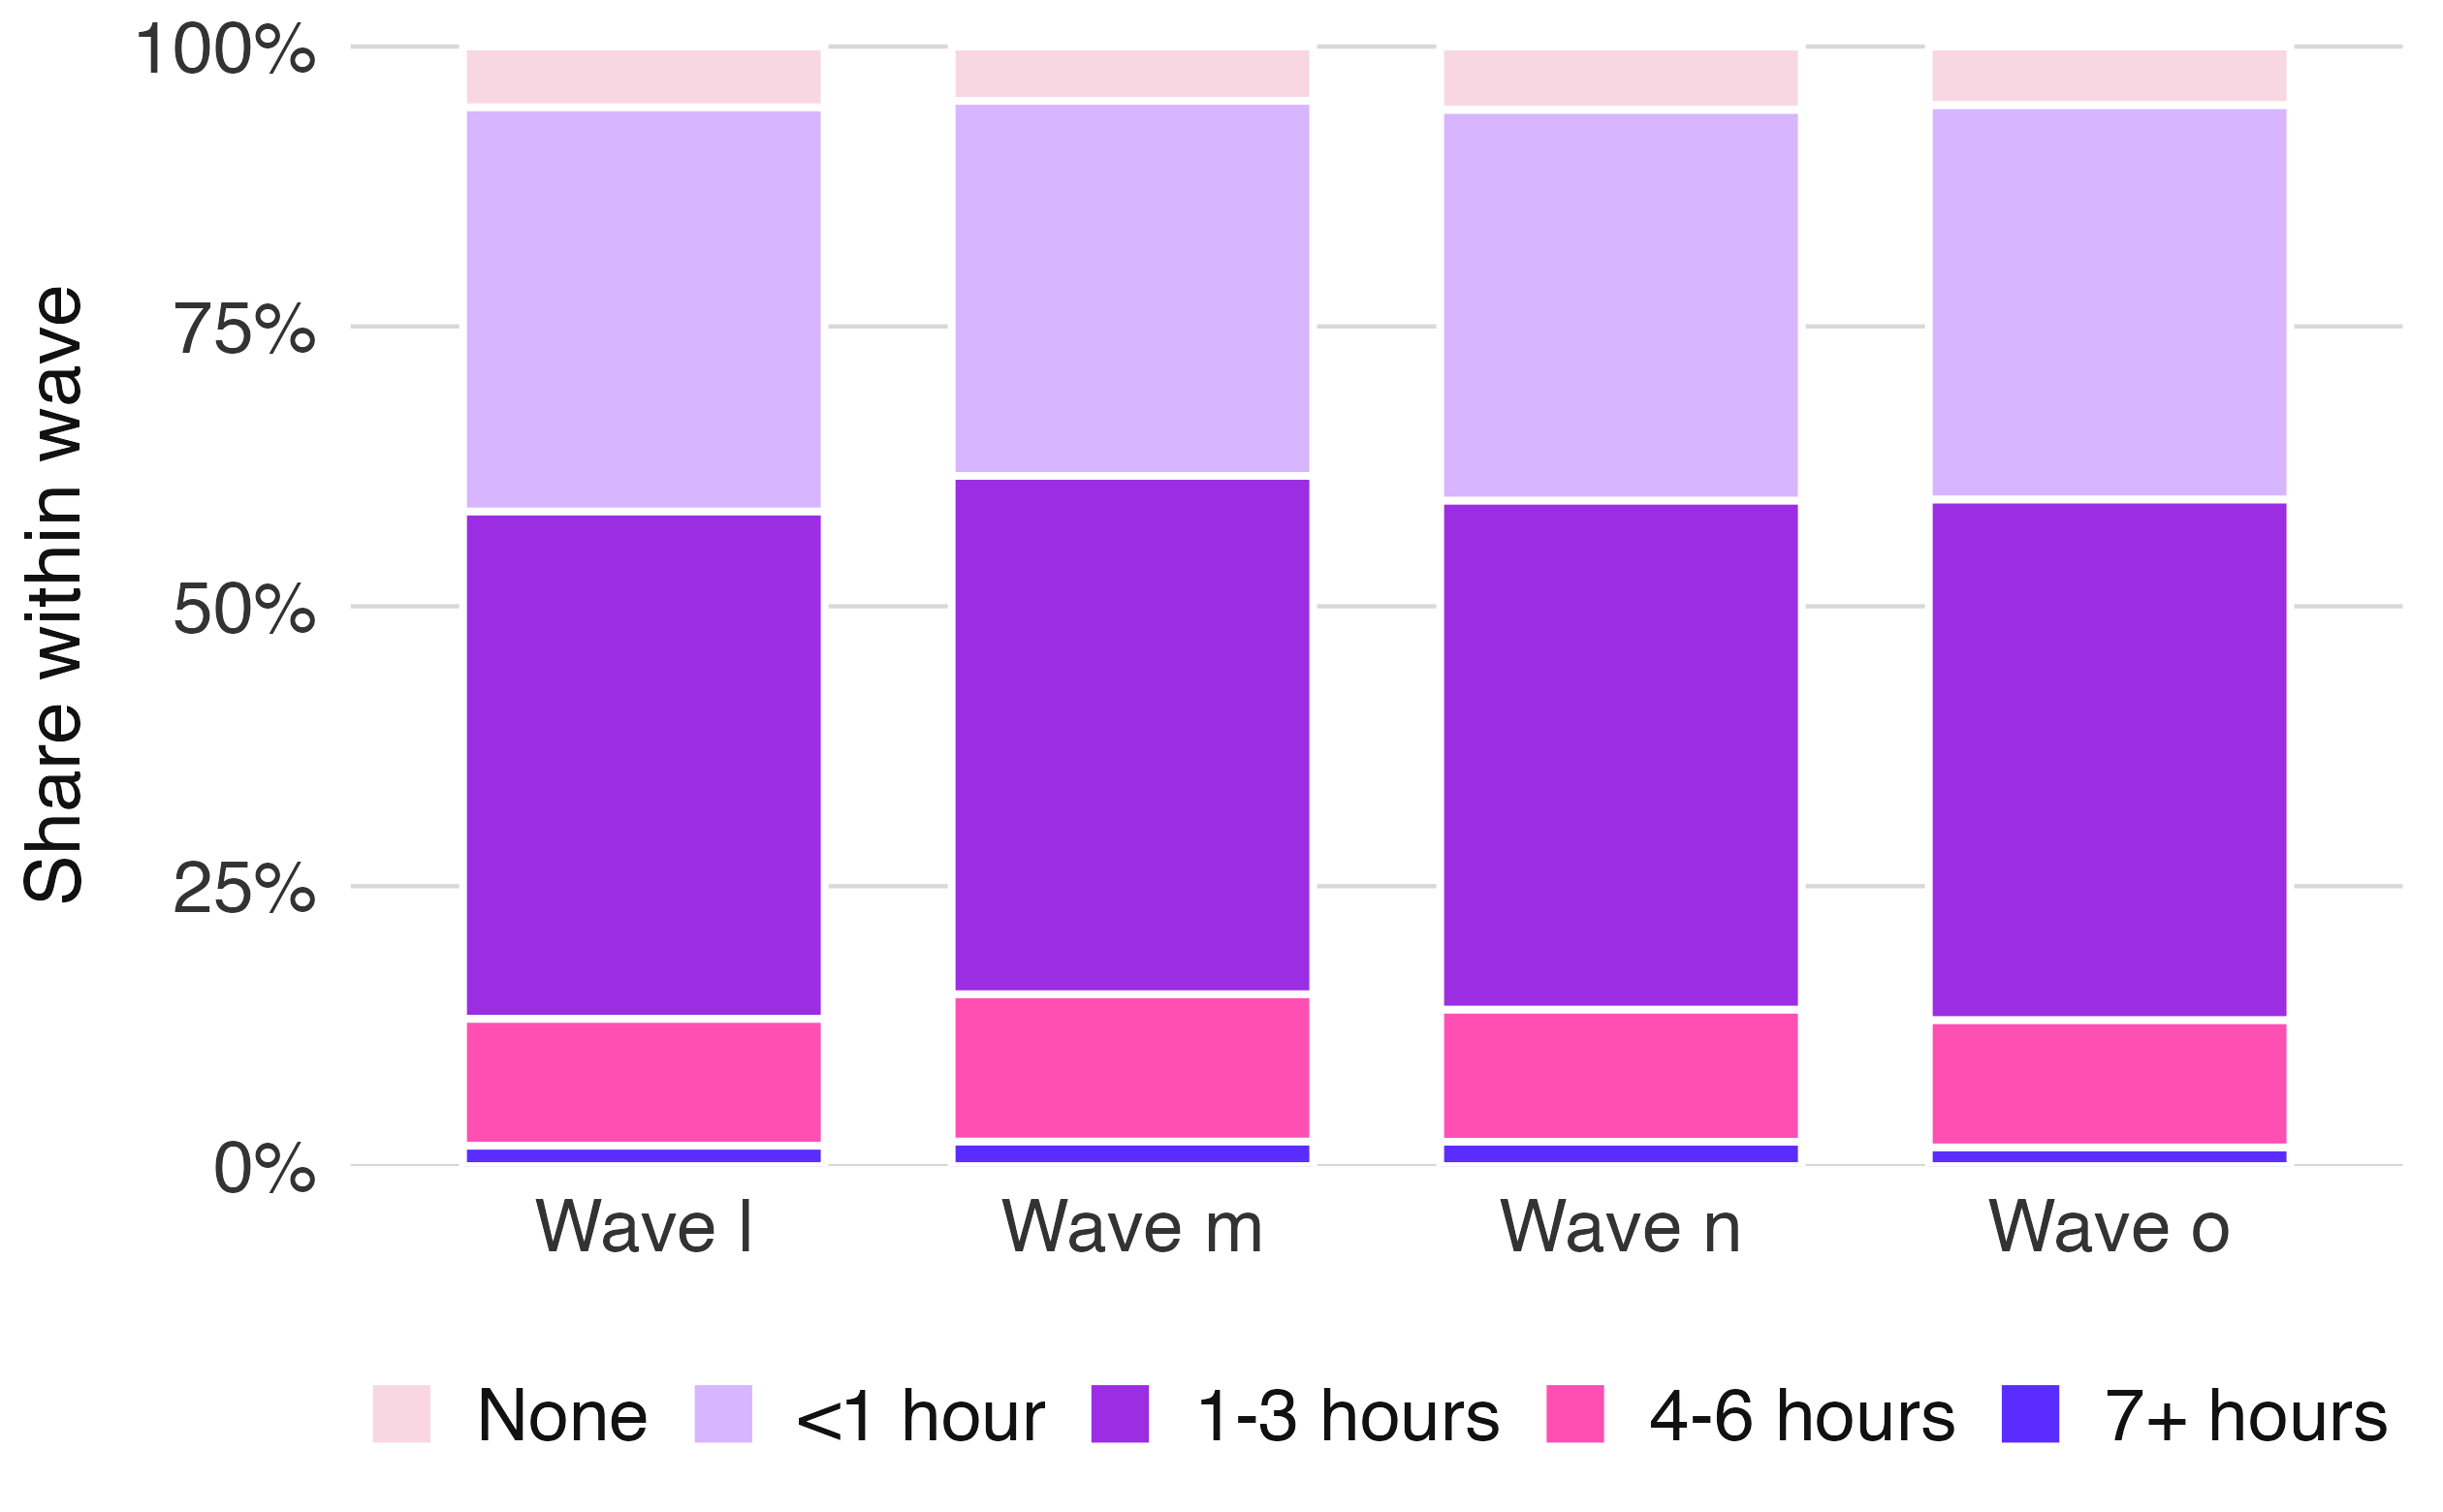
\includegraphics[width=0.78\textwidth]{figures/descriptive_treatment_distribution_by_wave_presentation.png}
\caption{Distribution of weekday social-media use across Waves \texttt{l}--\texttt{o}.}
\label{fig:descriptive_treatment_distribution}
\end{figure}

\textit{Outcomes by treatment category.} Figure \ref{fig:descriptive_outcomes_by_treatment} reports unadjusted mean outcomes by weekday social-media-use category. Mean outcome values are generally higher in the heavier-use categories, especially for the dissatisfaction measures, and the gradient becomes visibly steeper at the upper end of the distribution. This pattern is broadly in line with a wider literature that often finds heavier social-media exposure to be associated with worse adolescent well-being, even though estimated effect sizes are often modest and the causal interpretation remains debated \citep{orbenprzybylski2019association,braghieri2022socialmedia,kerr2023digitalmedia}. These differences should not be interpreted causally.

\begin{figure}[!htbp]
\centering
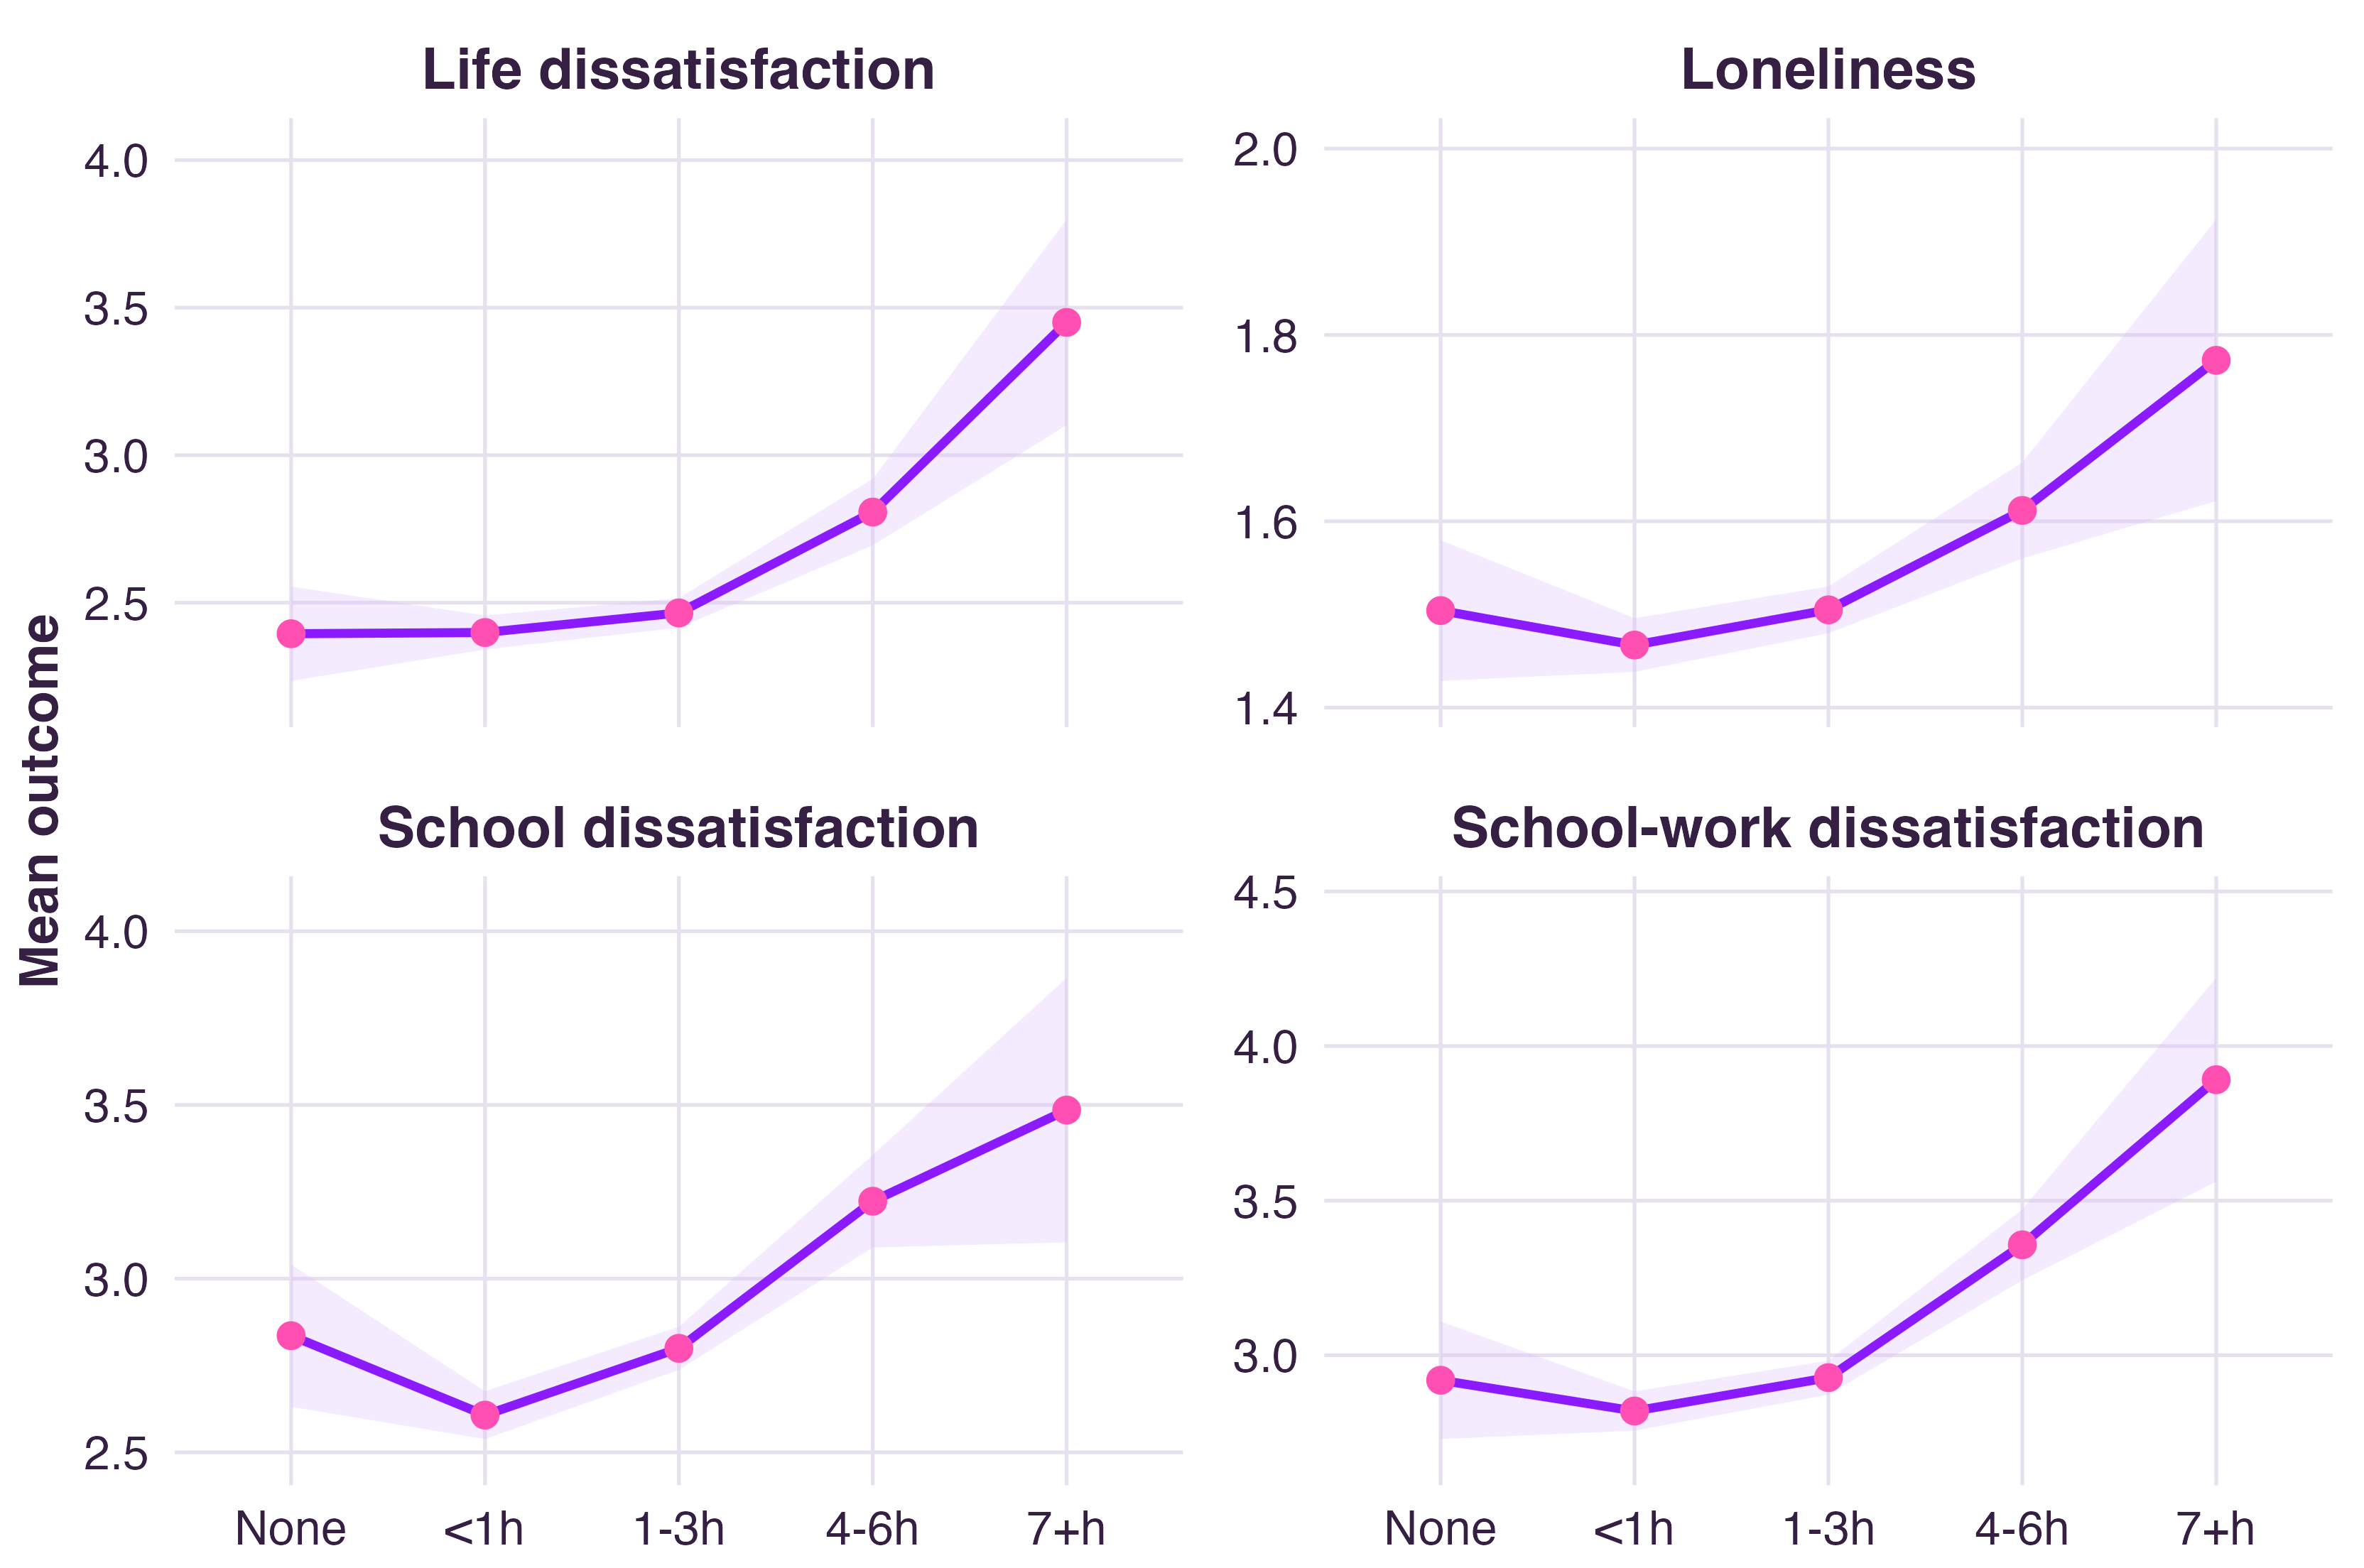
\includegraphics[width=0.8\textwidth]{figures/descriptive_outcomes_by_treatment_presentation.png}
\caption{Unadjusted mean wellbeing outcomes by weekday social-media-use category. Higher values indicate worse wellbeing.}
\label{fig:descriptive_outcomes_by_treatment}
\end{figure}

\textit{Age, sex, and social-media intensity.} Figure \ref{fig:descriptive_high_use_age_sex} restricts attention to ages 10--15, where the data are informative. Within that range, high weekday social-media use becomes more common at older ages. By contrast, differences by sex are modest and change sign across ages rather than following one stable pattern. The age gradient is consistent with broader evidence that digital and social-media use tends to rise across adolescence as smartphone-based communication becomes more central in daily life \citep{twenge2018newmedia}. Our sex split is flatter than in some other large adolescent datasets, in which girls more often report frequent social-media use than boys \citep{kerr2023digitalmedia}. 

\begin{figure}[!htbp]
\centering
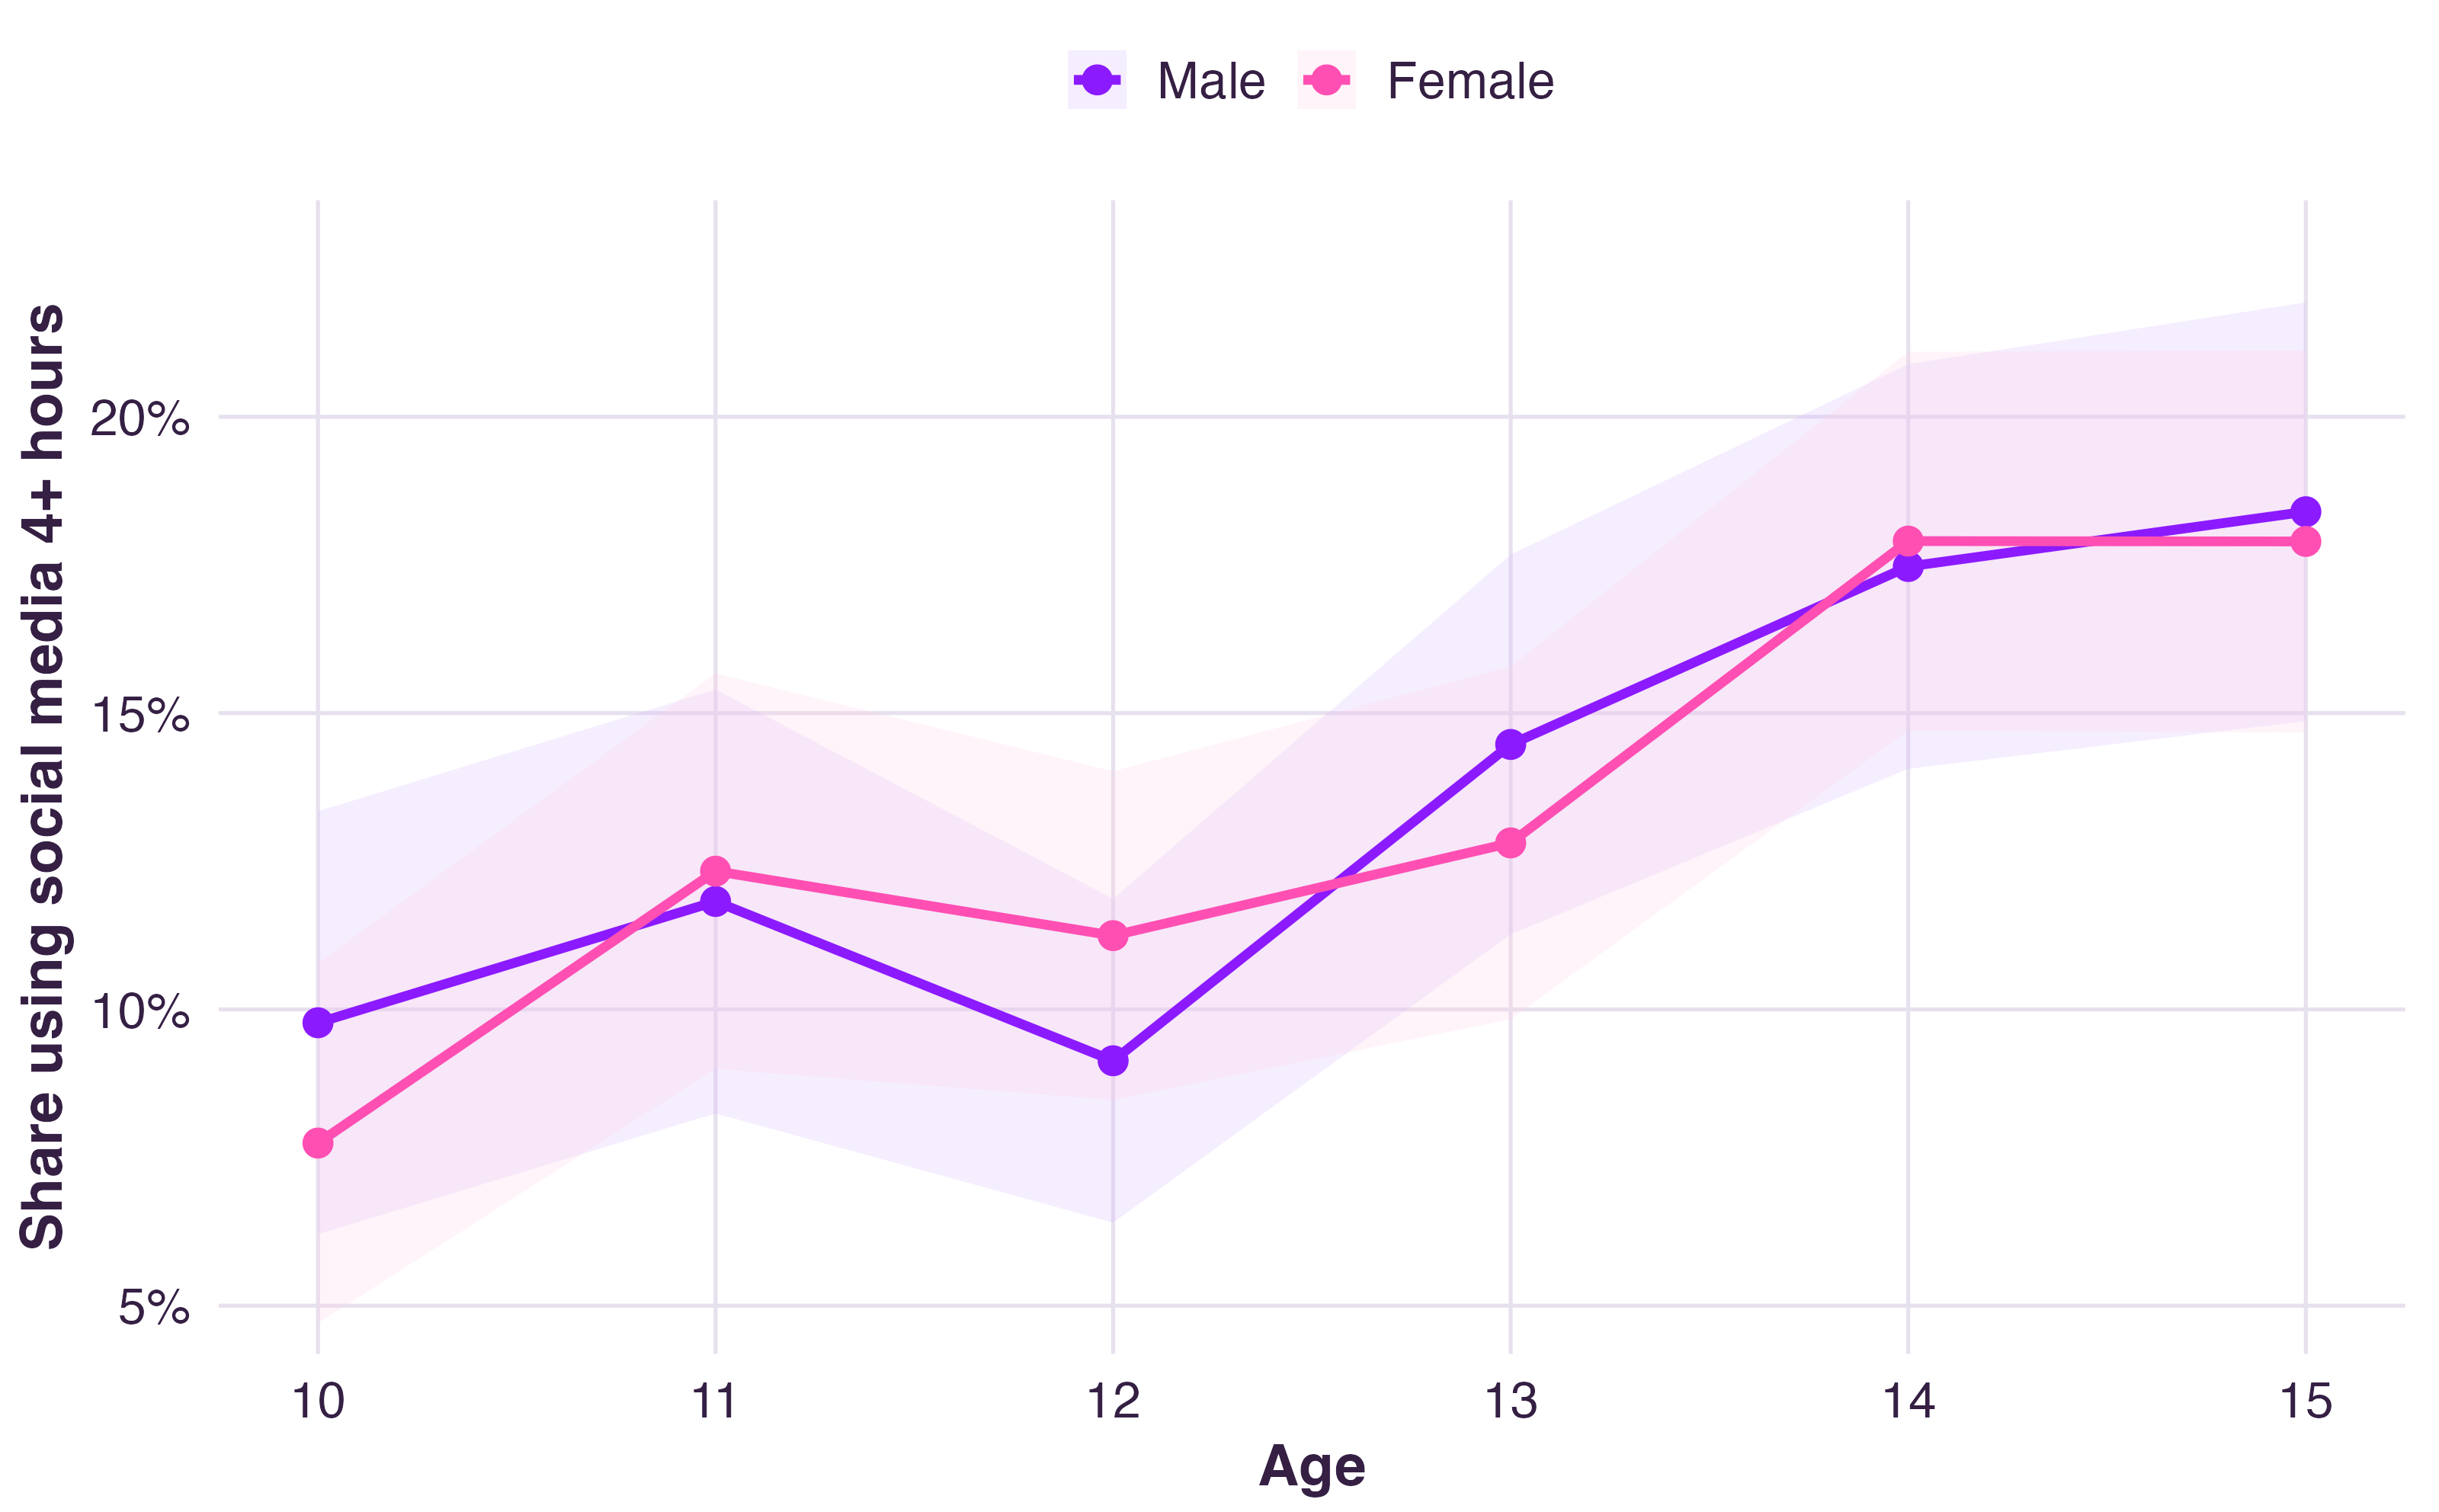
\includegraphics[width=0.78\textwidth]{figures/descriptive_high_use_by_age_and_sex_presentation.png}
\caption{Share reporting high weekday social-media use by age and sex for ages 10--15. High use is defined as at least four hours per weekday.}
\label{fig:descriptive_high_use_age_sex}
\end{figure}

\textit{Household routines and media environment.} Figure \ref{fig:descriptive_high_use_controls} shows that high use is more common among adolescents who report less frequent family meals and among those who report more television/video time. The family-meal gradient is consistent with a broader family-routines literature in which shared meals proxy family connectedness and supervision, as well as with pediatric media guidance that emphasizes screen-free family routines and designated screen-free times \citep{neumark2008familymeals,moreno2016mediause}. The positive television/video gradient is also plausible in light of evidence that screen-based sedentary behaviours often cluster within broader high-media-use profiles rather than occurring in isolation \citep{sisson2009sedentaryprofiles}.

\begin{figure}[!htbp]
\centering
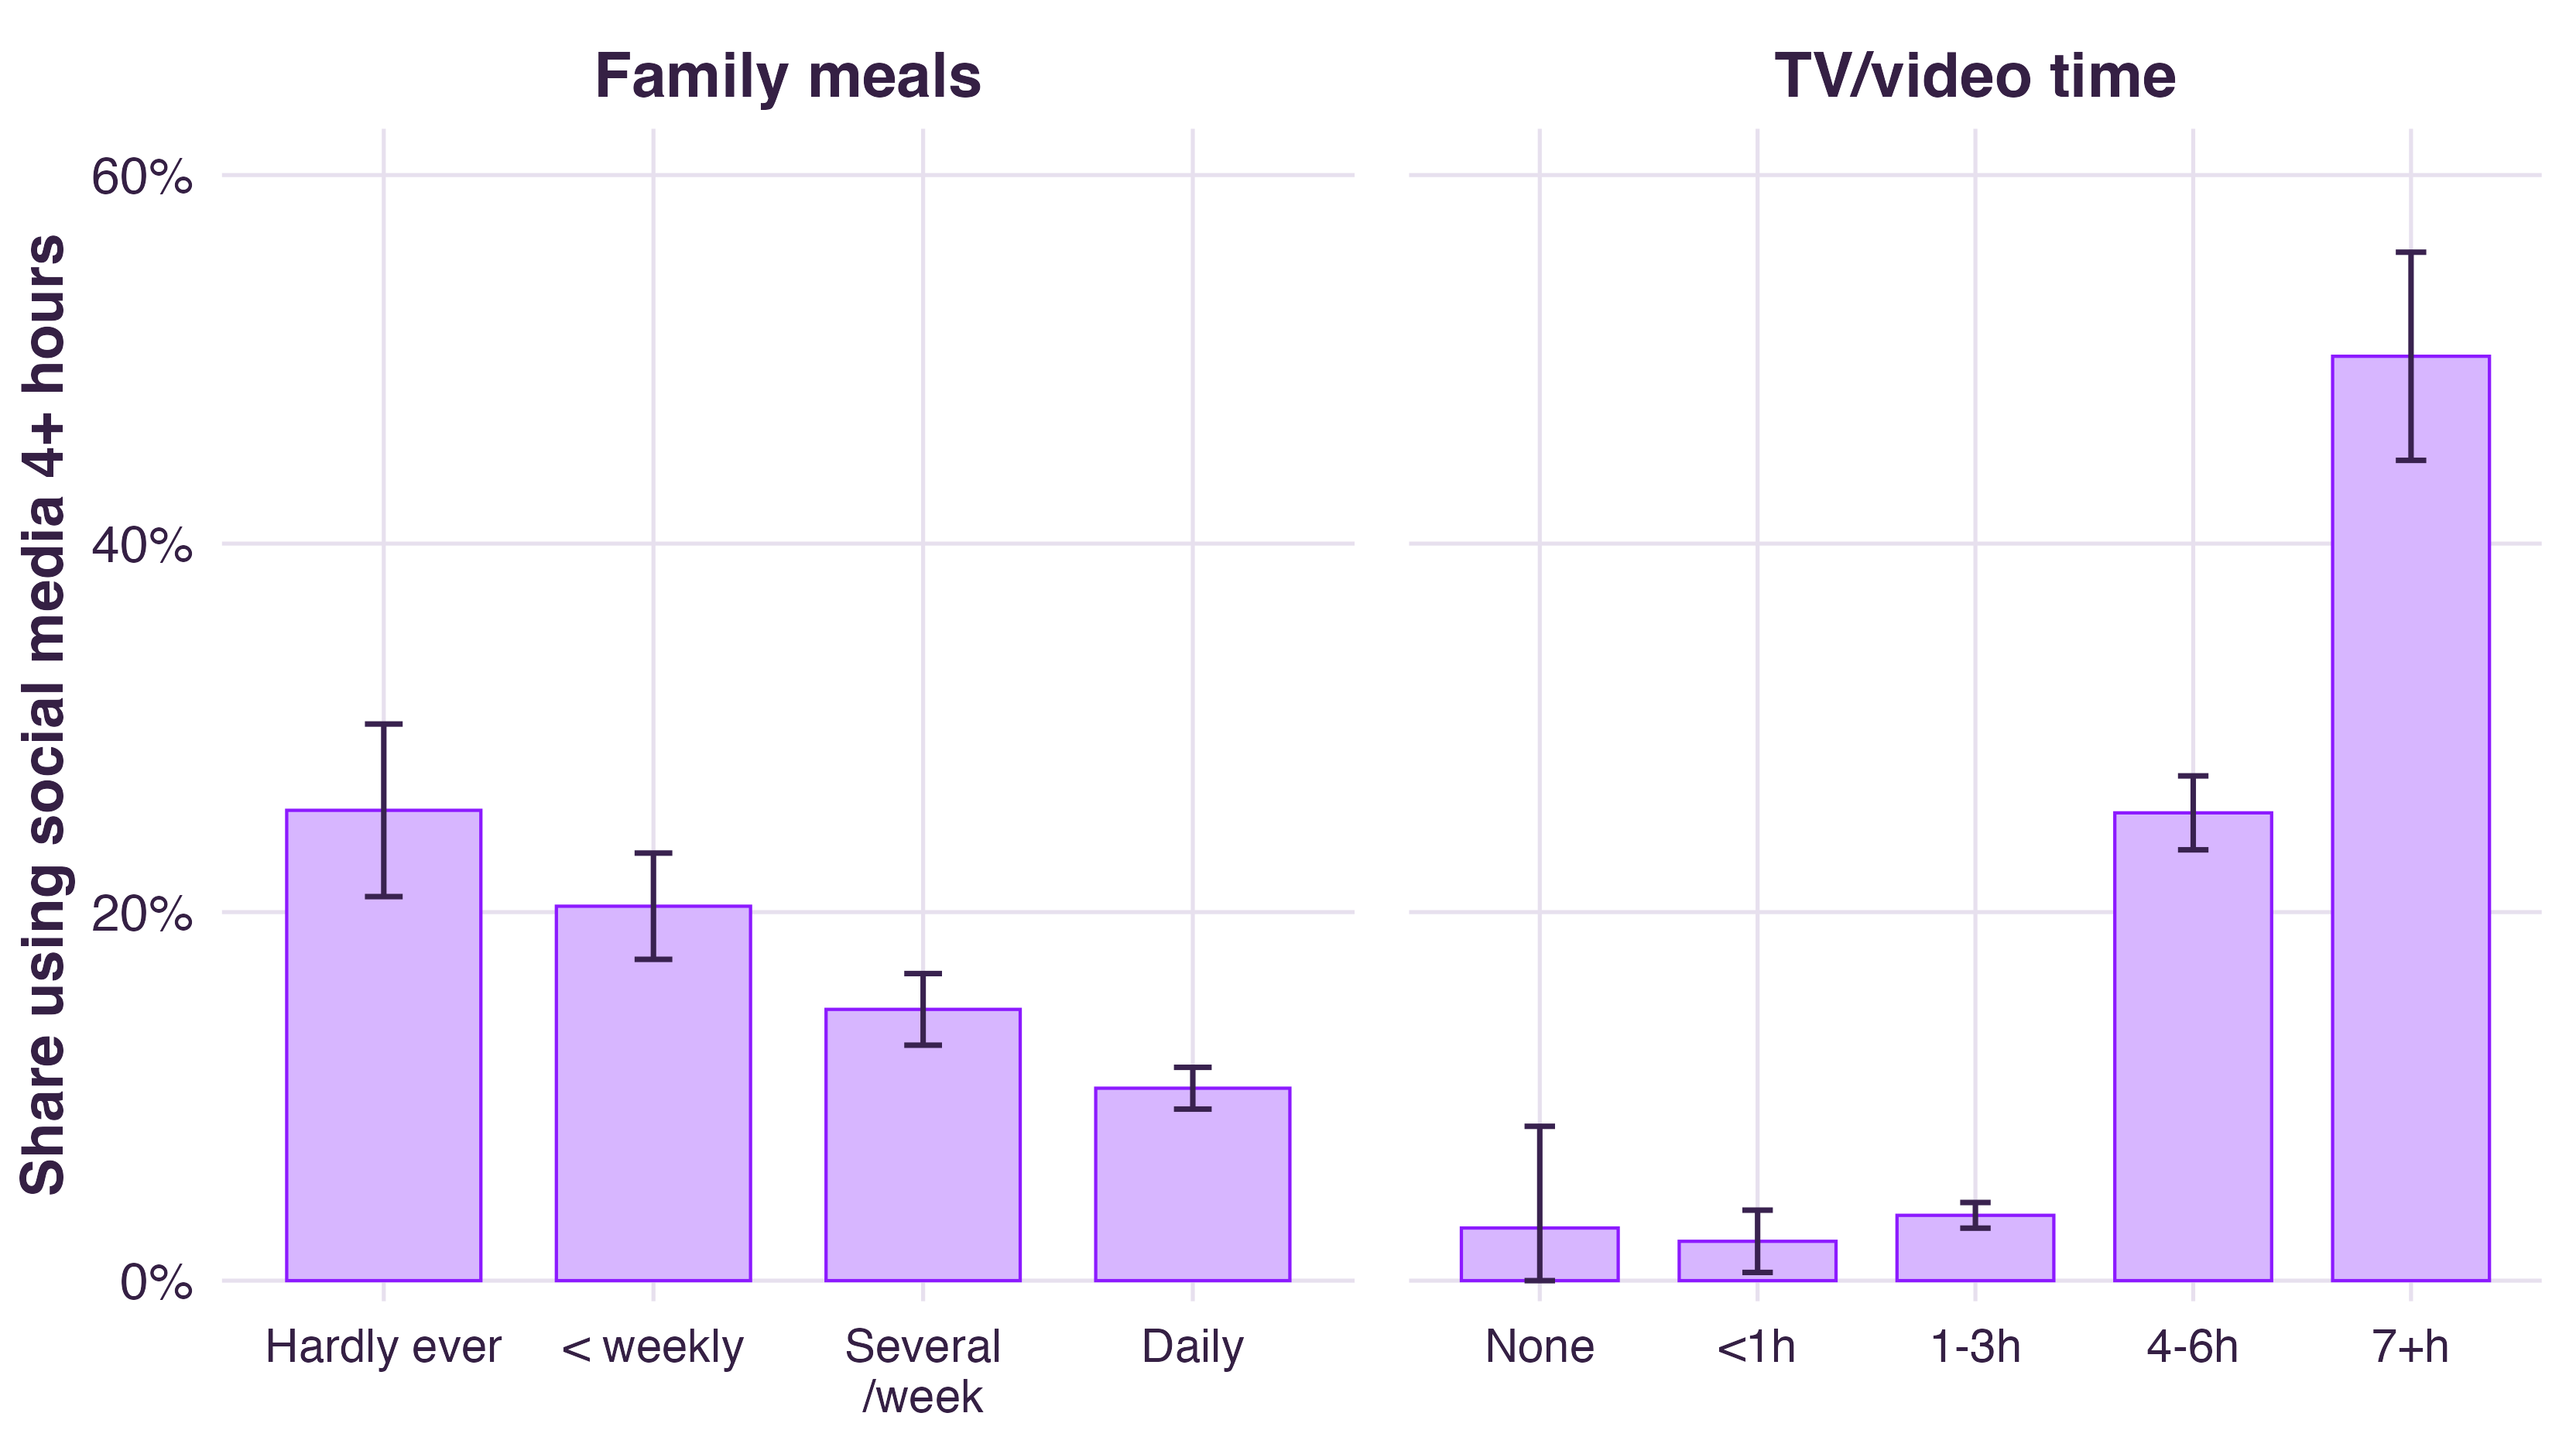
\includegraphics[width=0.76\textwidth]{figures/descriptive_high_use_by_controls_presentation.png}
\caption{Share reporting high weekday social-media use by family-meal frequency and television/video time. Whiskers show 95\% confidence intervals.}
\label{fig:descriptive_high_use_controls}
\end{figure}

\textit{Household composition.} Figure \ref{fig:descriptive_high_use_household} extends this comparison to household-composition controls. High use is lowest in two-parent households and somewhat higher when fewer parent figures are present. The grandparent and sibling panels show additional variation across household structures, although uncertainty is wider for the relatively small group living with a grandparent. The parent-figure gradient is consistent with literature on parental mediation and monitoring, which generally finds that clearer and more consistent family rules and involvement are associated with less problematic digital-media use among adolescents \citep{chen2019reducingharm,meeus2019constantly}. 

\begin{figure}[!htbp]
\centering
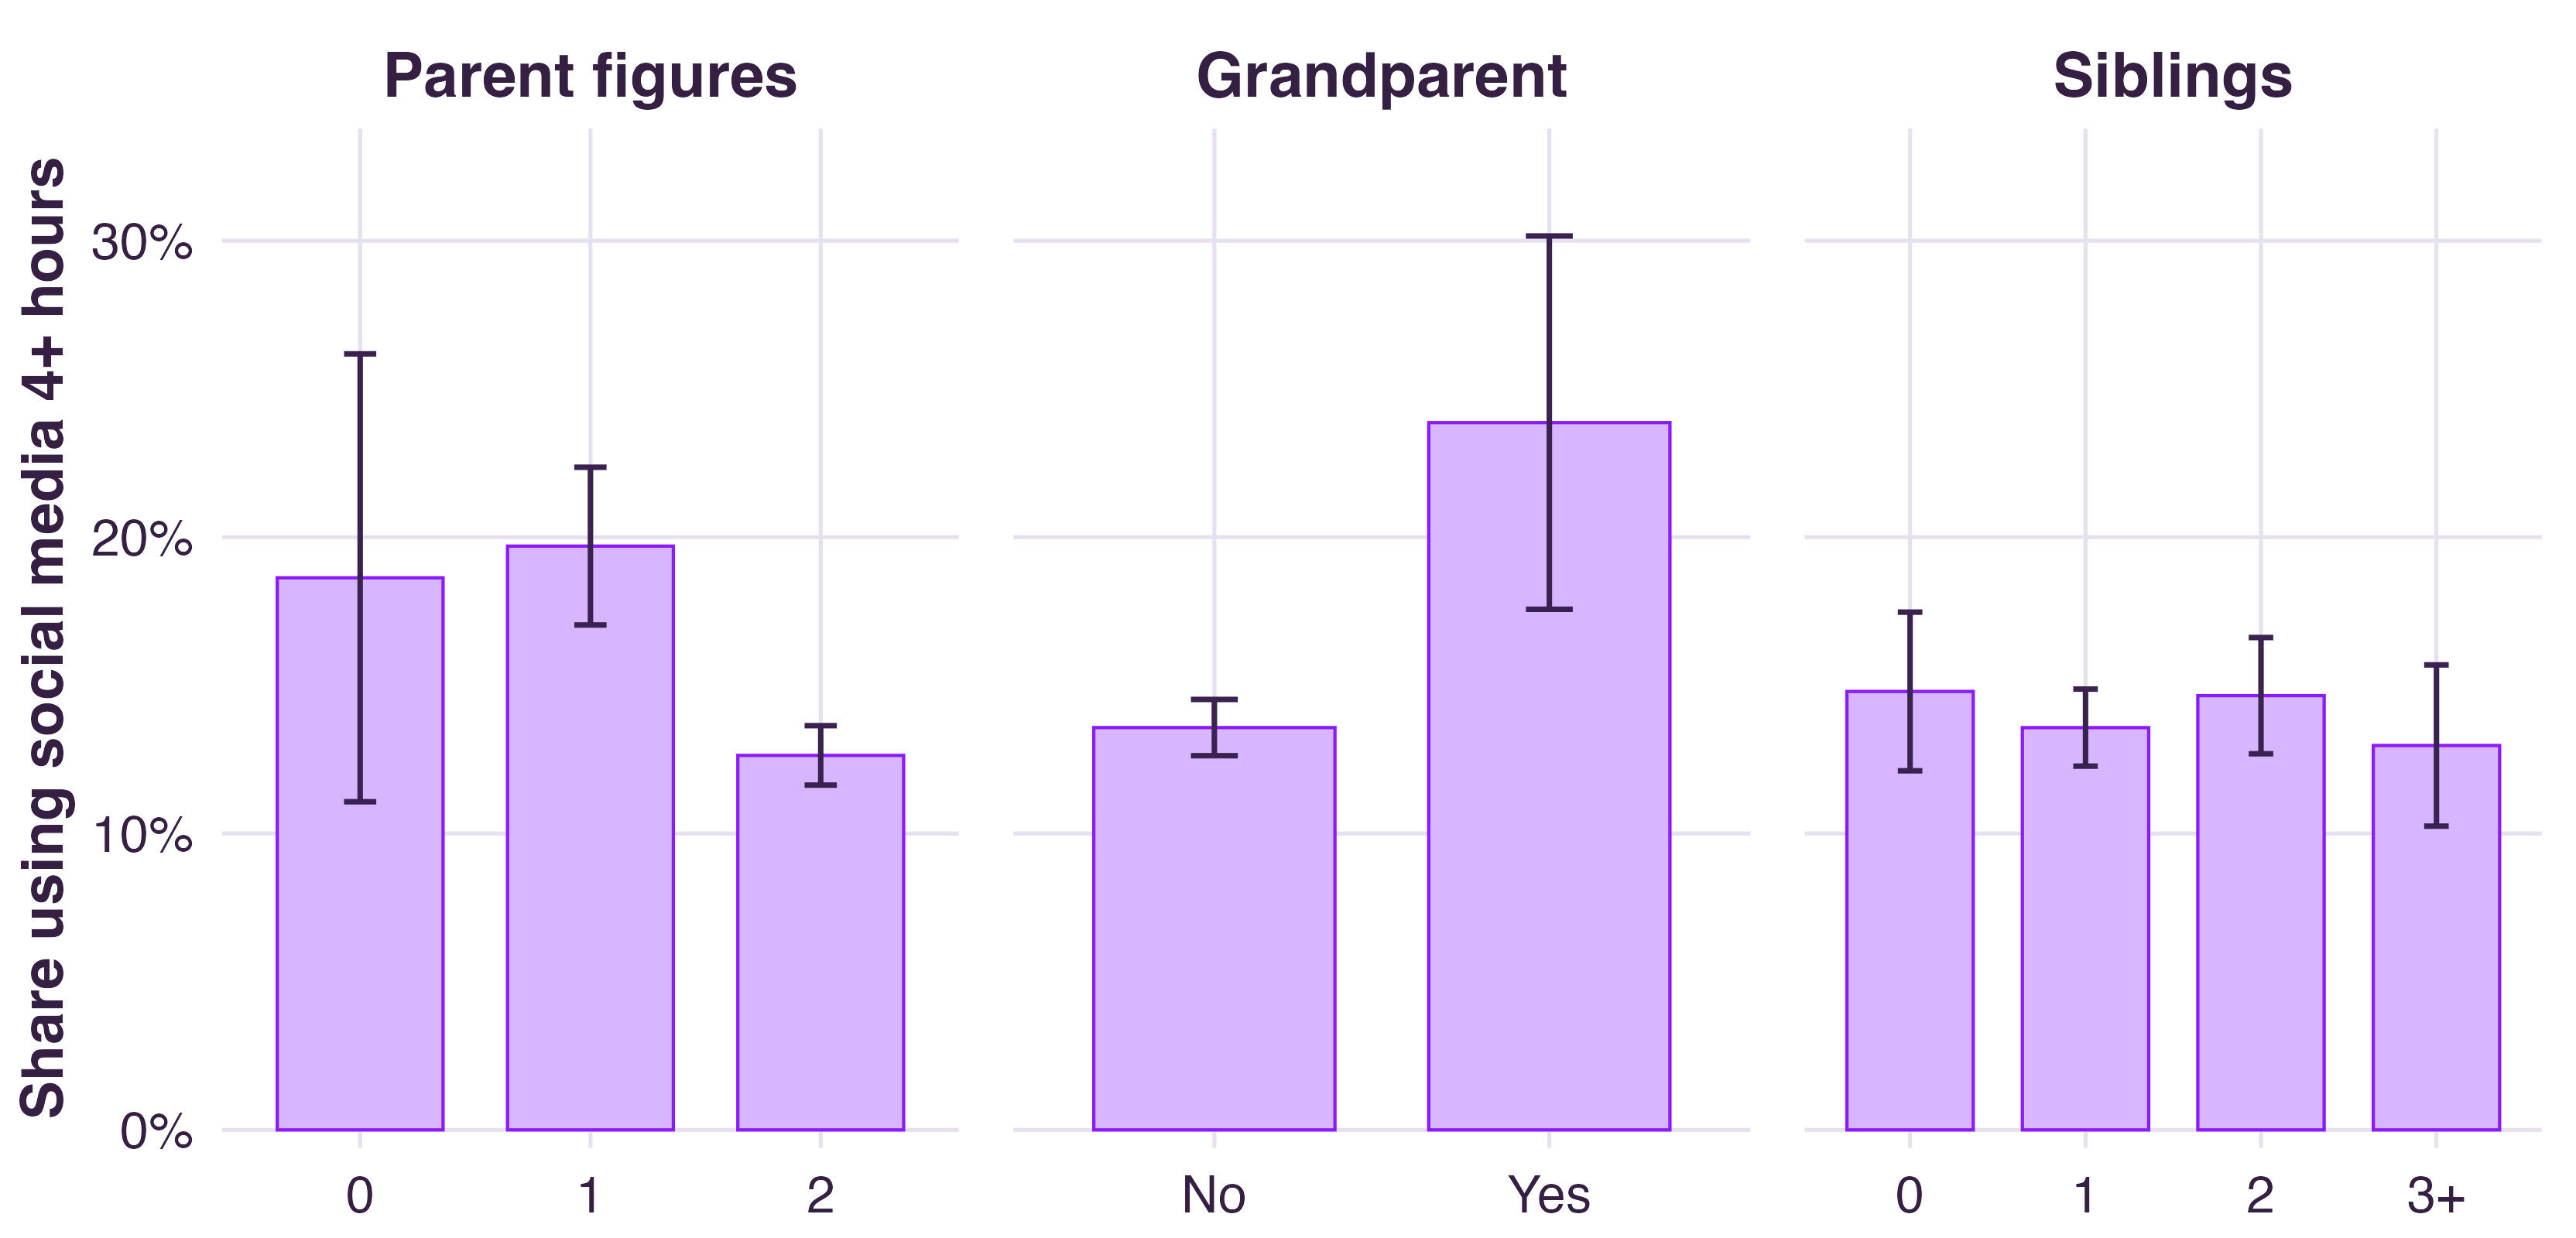
\includegraphics[width=0.66\textwidth]{figures/descriptive_high_use_by_household_presentation.png}
\caption{Share reporting high weekday social-media use by household composition. Whiskers show 95\% confidence intervals.}
\label{fig:descriptive_high_use_household}
\end{figure}

\FloatBarrier

Taken together, the descriptive evidence emphasizes two features for the subsequent empirical analysis. First, treatment variation is substantial in every wave. Second, heavier weekday social-media use is systematically related to age, household routines, broader media exposure, and household structure.

\tocchapter{Theoretical Framework}{Theoretical framework}
\label{chap:theory}

This chapter outlines the econometric framework for the analysis. It explains why causal inference is challenging in observational data, how standard panel estimators exploit the longitudinal design to control for unobserved heterogeneity, and why double machine learning can be a useful extension when the set of controls is high-dimensional and functional-form assumptions are uncertain.

\tocsection{Panel Models for Repeated Observations}{Panel models for repeated observations}

A central challenge is that social-media usage is not randomly assigned: adolescents who spend more time online may systematically differ in family routines, peer networks, device access, local environment, or inherent personality traits from those who use it less. Ordinary least squares (OLS) regression is a natural starting point, but it relies on observing sufficiently rich confounders and modeling their effects correctly. A basic pooled linear panel model is
\begin{equation*}
Y_{it} = \alpha + \beta X_{it} + Z_{it}'\gamma + \varepsilon_{it},
\end{equation*}
where \(Y_{it}\) denotes the outcome variable, \(X_{it}\) the treatment variable of interest, and \(Z_{it}\) the vector of observed controls. This model pools all individuals and waves together, assuming common intercept and slope coefficients across subjects and time.\\
\\
\textbf{Why pooled regression may be misleading}\\
\\
Pooling observations increases sample size and precision, but it also introduces correlation among repeated measures of the same individual \citep{ward1993pooled}. Ignoring this respondent-specific correlation can lead to biased or inefficient estimates and invalid standard errors. In other words, pooled OLS is informative as a starting point but can be misleading if heterogeneity is not accounted for.\\
\\
\textbf{Controlling for stable adolescent heterogeneity}\\
\\
To control for unobserved time-invariant heterogeneity, one can use fixed-effects or random-effects models \citep{ward1993pooled,baltagi2013panel}. The fixed-effects model adds individual-specific intercepts:
\begin{equation*}
Y_{it} = \alpha_i + \beta X_{it} + Z_{it}'\gamma + \varepsilon_{it},
\end{equation*}
and can also include wave fixed effects ($\lambda_t$) to capture common time shocks:
\begin{equation*}
Y_{it} = \alpha_i + \lambda_t + \beta X_{it} + Z_{it}'\gamma + \varepsilon_{it}.
\end{equation*}
Identification of $\beta$ in this specification comes purely from within-adolescent changes over time, effectively differencing out any time-constant factors. By contrast, the random-effects model treats the individual intercept as a random component of the error:
\begin{align*}
Y_{it} &= \alpha + \beta X_{it} + Z_{it}'\gamma + v_{it}, \\
v_{it} &= u_i + \varepsilon_{it},
\end{align*}
where $u_i$ is the time-invariant individual effect and $\varepsilon_{it}$ is the idiosyncratic error. Random-effects estimation is more efficient if $u_i$ is uncorrelated with the regressors, but this orthogonality assumption may not hold in practice. Figure \ref{fig:panel_model_schematic} illustrates the intuition behind these models. In our context, fixed effects is often preferred because stable adolescent characteristics (such as family background or temperament) are likely correlated with both social-media use and well-being \citep{ward1993pooled,wooldridge2010panel}.

\begin{figure}[!htbp]
\centering
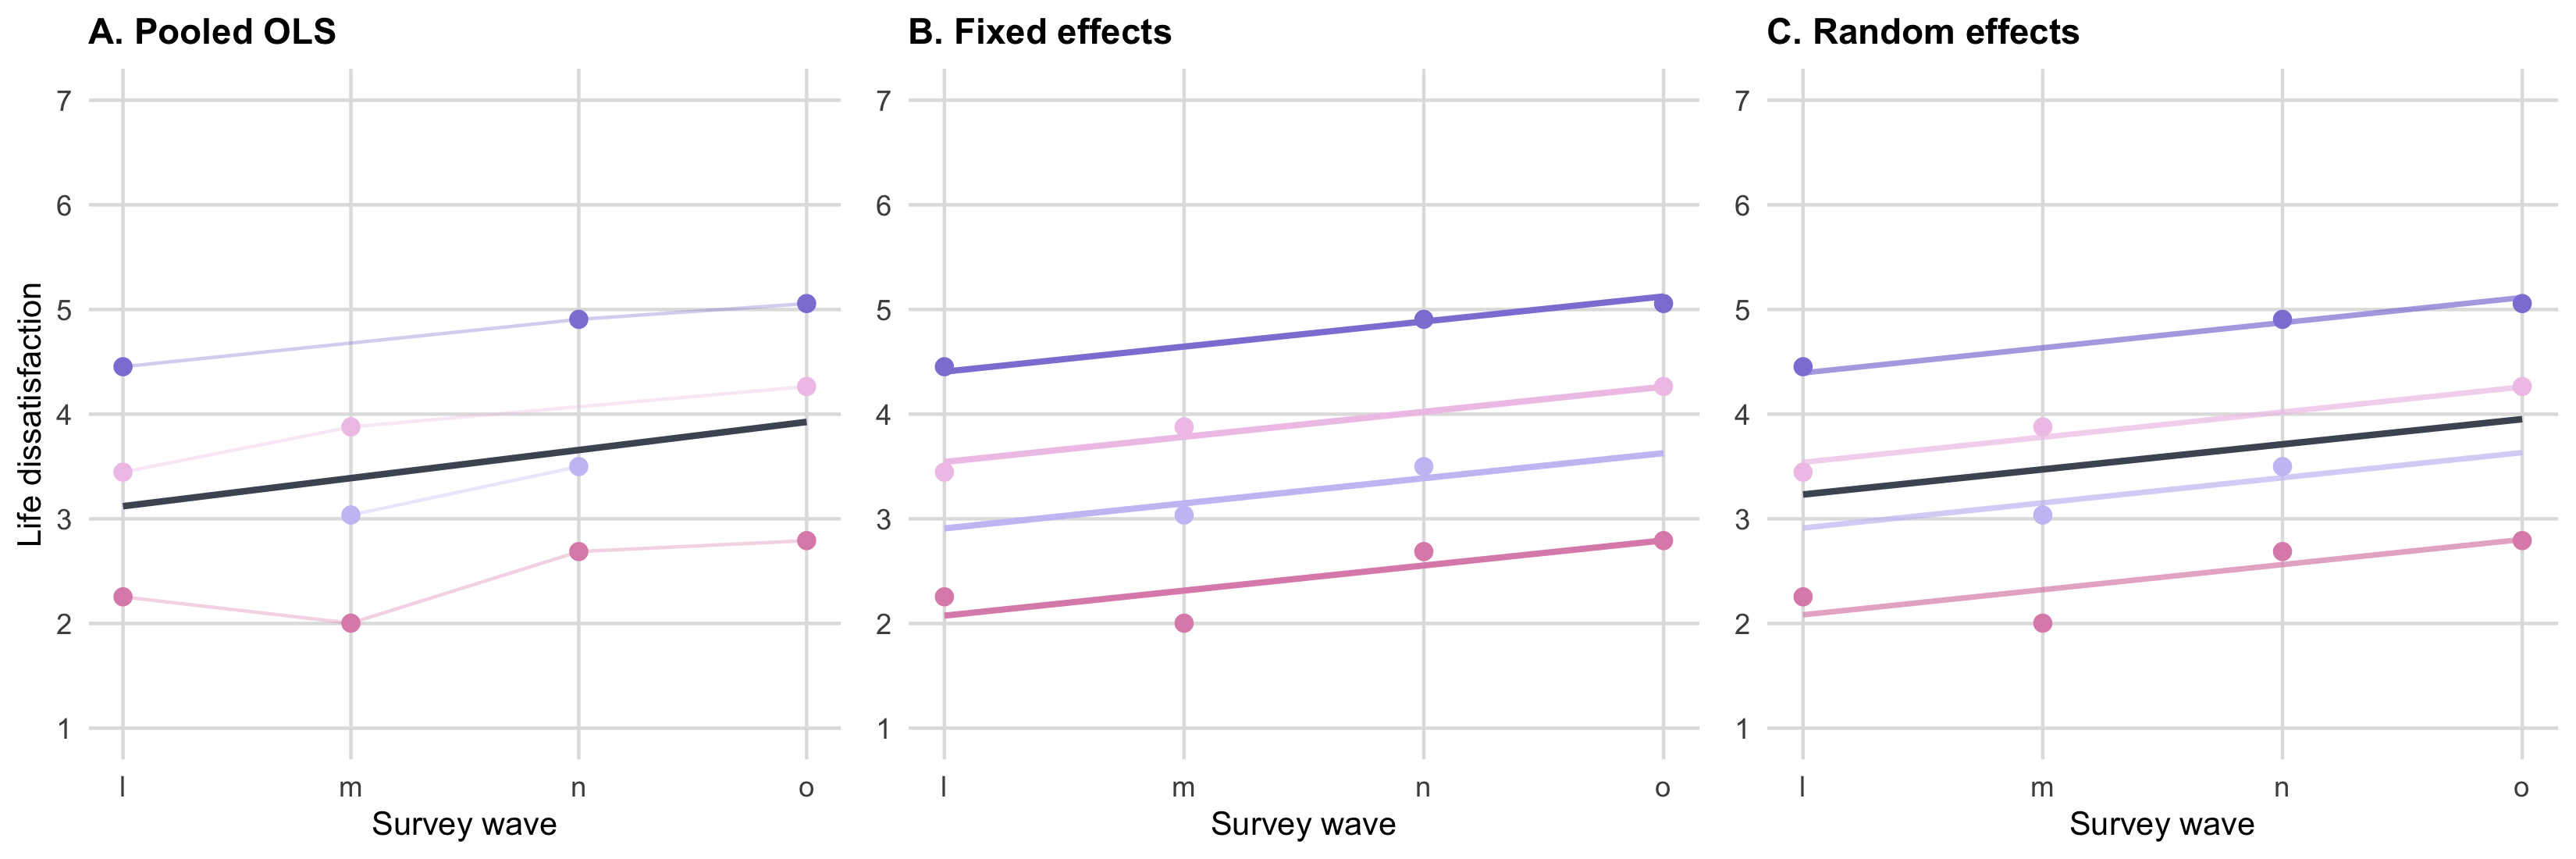
\includegraphics[width=0.95\textwidth]{figures/panel_model_schematic.png}
\caption{Stylized comparison of pooled OLS, fixed effects, and random effects for life dissatisfaction over Waves \texttt{l}--\texttt{o}. The toy panel is intentionally unbalanced, so some adolescents are observed in only two or three waves. Panel A fits one common regression line to the pooled data. Panel B allows adolescent-specific intercepts while keeping a common slope. Panel C combines a common population line with adolescent-specific random-intercept deviations.}
\label{fig:panel_model_schematic}
\end{figure}\noindent
\textbf{Selecting the preferred linear panel model}
\label{sec:choice_model_spec}\\
\\
Choosing between pooled OLS, fixed-effects, and random-effects models can be guided by standard specification tests \citep{ward1993pooled,baltagi2013panel}. A global F-test compares fixed effects with pooled OLS by asking whether the respondent-specific intercepts jointly improve fit. A Breusch--Pagan Lagrange Multiplier test compares random effects with pooled OLS by testing whether a respondent-level variance component is needed. The Hausman test then compares  fixed versus random effects by checking for systematic differences in estimated coefficients; a significant difference suggests that the random-effects assumption may be violated. In practice, these tests complement substantive reasoning about the data-generating process but do not replace it. Appendix~\ref{app:spec_tests} provides the formulas and critical values for these tests.

\tocsection{Double Machine Learning for Flexible Confounder Adjustment}{Double machine learning for flexible confounder adjustment}
\label{sec:dml_background}

Standard panel estimators remain valuable because they show how the estimated effect of social-media use changes when richer controls and individual heterogeneity are introduced. However, these models typically impose restrictive functional-form assumptions on the controls. When the control vector is high-dimensional, forcing variables such as age, geography, household composition, peer environment, device access, and survey wave into a simple additive linear structure can itself introduce misspecification \citep{athey2019mlmethods,baiardi2024valueadded,knaus2021musicdml,helal2026returns}.\\
\\
\textbf{Observed confounding and functional-form misspecification}\\
\\
Experimental variation is often unavailable in social-science research due to feasibility, cost, or ethical constraints. Consequently, researchers frequently rely on observational data and invoke a conditional-independence assumption: after conditioning on a sufficiently rich set of observed confounders, the remaining treatment variation is assumed to be independent of potential outcomes \citep{atheyimbens2017state,imbens2004nonparametric,helal2026returns}. The credibility of an observational analysis thus depends on whether the relevant confounders are observed and on whether their relationships with the treatment and the outcome are correctly modeled.


This requirement becomes especially demanding when the control set is large. A conventional regression model forces the researcher to decide a priori how each variable (for example, age) enters the equation (linearly or nonlinearly), which interactions to include, and where threshold effects might occur. Misspecifying these relationships can leave residual confounding even if the relevant variables are present. In our application, factors such as age, household structure, peer environment, screen habits, device access, and survey wave may jointly influence both social-media use and adolescent well-being. This motivates using methods that can represent these adjustment relationships more flexibly \citep{athey2019mlmethods,fuhr2024dml,helal2026returns}.\\
\\
\textbf{Machine learning for flexible nuisance-function estimation}\\
\\
Supervised machine-learning methods estimate relationships between predictors and an observed response with the primary goal of minimizing prediction error. A learner estimates
\begin{equation*}
\widehat{Y} = \widehat{f}(X),
\end{equation*}
where \(\widehat{f}\) is learned from the data without being restricted to a pre-specified linear-additive form. For example, tree-based learners partition the covariate space into regions and can automatically capture threshold effects and interactions. Random forests stabilize this process by averaging predictions across many trees built from resampled data and random subsets of predictors \citep{athey2019mlmethods}. Neural networks achieve flexibility through layered nonlinear transformations. Such methods can thus approximate complex nuisance functions that simple parametric models might miss \citep{mullainathan2017machine,helal2026returns}.

This flexibility entails a bias–variance trade-off. A learner that fits too closely to the training data may overfit noise and perform poorly on new data. Modern algorithms therefore control complexity through mechanisms such as limiting tree depth, enforcing minimum leaf sizes, subsampling features, applying weight decay or dropout, or using early stopping. These constraints can be formalized in a regularized empirical-risk minimization problem: 
\begin{equation*}
\widehat{f}
=
\arg\min_{f\in\mathcal{F}}
\left\{
\frac{1}{n}\sum_{j=1}^{n}L\!\left(Y_j,f(X_j)\right)
+\lambda\Omega(f)
\right\},
\end{equation*}
where \(L(\cdot)\) is a prediction loss, \(\mathcal{F}\) is the function class (learner family), \(\Omega(f)\) measures model complexity, and \(\lambda\) determines the strength of regularization.\footnote{The precise form of regularization differs across learners. For a regression tree it may operate through restrictions on depth and leaf-size; for a neural network it may operate through weight decay or early stopping. The empirical learners and their tuning parameters are described in Chapter \ref{chap:methodology}.} Regularization generally improves out-of-sample stability, but it also means that the fitted nuisance function need not match the true function at every point, introducing bias \citep{chernozhukov2018dml,fuhr2024dml,helal2026returns}.\\
\\
\textbf{Why accurate prediction is insufficient for causal estimation}\\
\\
Prediction and causal estimation serve different purposes. A predictive model is evaluated by its accuracy in forecasting outcomes for new data, whereas our goal is to estimate a low-dimensional parameter: the causal effect of the treatment after adjusting for confounders. A model may achieve high predictive accuracy for mental well-being yet fail to provide a valid estimate of the social-media effect \citep{shmueli2010explain,mullainathan2017machine,helal2026returns}.

This distinction becomes especially important when regularized predictions are plugged into a conventional estimating equation. Prediction errors in the treatment and outcome models can then spill into the treatment coefficient in first order. Thus, good predictive performance alone does not guarantee that the regularization bias is negligible or that standard errors from an ordinary regression remain valid \citep{belloni2014highdim,chernozhukov2018dml}. The econometric task is to combine flexible nuisance estimation with a strategy that protects the low-dimensional treatment parameter from these first-order errors. Double/debiased machine learning achieves this objective \citep{helal2026returns}.\\
\\
\textbf{The double machine learning framework}\\
\\
Double/debiased machine learning builds on earlier work on high-dimensional treatment-effect estimation and post-double selection \citep{belloni2014highdim}. Chernozhukov et al.\ generalize this logic beyond one specific learner by allowing a broad class of machine-learning methods to estimate nuisance functions, while protecting the target parameter via Neyman-orthogonal scores and cross-fitting \citep{chernozhukov2018dml}. In the partially linear model considered in Chapter \ref{chap:methodology}, the structure is
\begin{align*}
Y_{it} &= \beta_0 D_{it} + g_0(X_{it}) + U_{it}, \\
D_{it} &= m_0(X_{it}) + V_{it},
\end{align*}
where \(Y_{it}\) denotes the outcome for individual $i$ in wave $t$, \(D_{it}\) the treatment, and \(X_{it}\) the observed controls. The functions \(g_0(X_{it})\) and \(m_0(X_{it})=\mathbb{E}[D_{it}\mid X_{it}]\) are nuisance functions: they are needed to identify \(\beta_0\), but are not themselves the main parameters of interest.

\begin{figure}[!htbp]
\centering
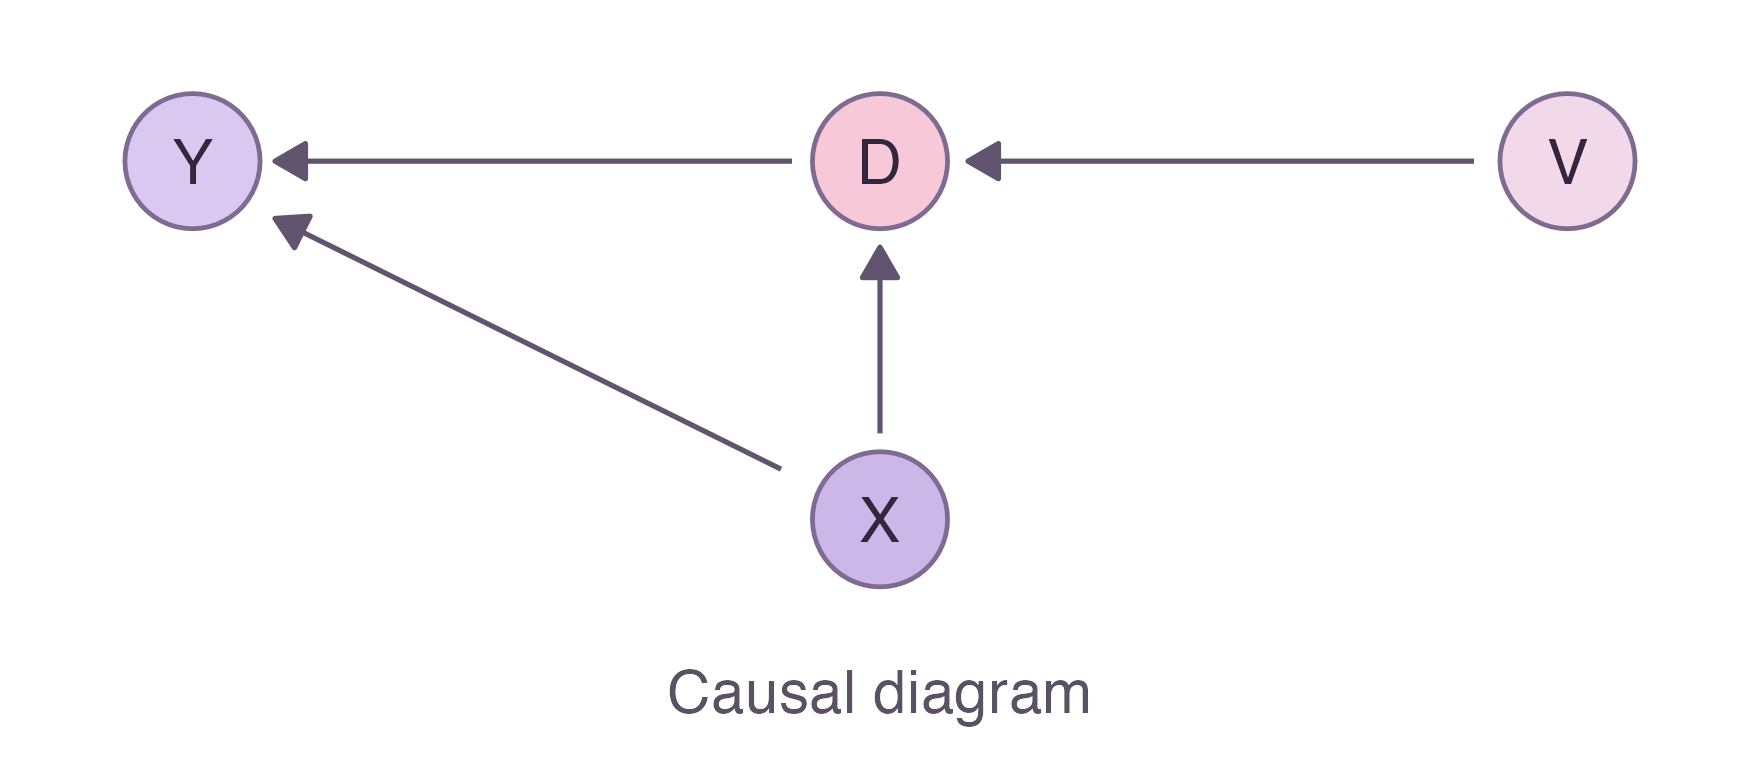
\includegraphics[width=0.73\textwidth]{figures/causal_diagram_plr.png}
\caption{Causal diagram for the partially linear model. The observed controls \(X_{it}\) affect both the treatment \(D_{it}\) and the outcome \(Y_{it}\), while \(V_{it}\) denotes the residual treatment variation after conditioning on \(X_{it}\).}
\label{fig:causal_diagram_plr}
\end{figure}

Figure \ref{fig:causal_diagram_plr} illustrates the generic identification structure. The arrow from \(X_{it}\) to both \(D_{it}\) and \(Y_{it}\) represents observed confounding, whereas \(V_{it}\) is the component of the treatment not explained by \(X_{it}\). The parameter \(\beta_0\) is identified from the relationship between this residual treatment variation and the outcome after adjustment for the controls.

Define the conditional expectation of the outcome as
\begin{equation*}
\ell_0(X_{it})
:=
\mathbb{E}[Y_{it}\mid X_{it}]
=
\beta_0m_0(X_{it})+g_0(X_{it}).
\end{equation*}
The DML procedure flexibly learns \(\ell_0\) and \(m_0\), then purges their predicted values from the observed outcome and treatment. The remaining residuals are used to estimate \(\beta_0\). The estimating equation for \(\beta_0\) is constructed to be Neyman-orthogonal with respect to the nuisance functions, and it is evaluated using out-of-sample predictions of those functions \citep{chernozhukov2018dml,bach2024doubleml,helal2026returns}.\\
\\
\textbf{Orthogonalizing the treatment-effect estimator}\\
\\
For the partially linear model, the key orthogonal moment residualizes both the outcome and the treatment:
\begin{equation}
\mathbb{E}\!\left[
\left\{
Y_{it}-\ell_0(X_{it})
-\beta_0\bigl(D_{it}-m_0(X_{it})\bigr)
\right\}
\bigl(D_{it}-m_0(X_{it})\bigr)
\right]
=0.
\label{eq:dml_third_moment}
\end{equation}
Since \(Y_{it}-\ell_0(X_{it}) = U_{it}\) and \(D_{it}-m_0(X_{it}) = V_{it}\), this simplifies to \(\mathbb{E}[U_{it}V_{it}] = 0\).  Under \(\mathbb{E}[U_{it}\mid D_{it},X_{it}]=0\), it follows that \(\mathbb{E}[U_{it}V_{it}] = \mathbb{E}[V_{it}\mathbb{E}[U_{it}\mid D_{it},X_{it}]] = 0\). Appendix \ref{app:dml_derivations} derives this condition and examines alternative one-sided moments (residualizing only \(Y\) or only \(D\)), which serve as counterexamples: if one residualizes only one side, the estimation error in the nuisance model can enter the treatment effect estimate at first order \citep{chernozhukov2018dml}.

Equation \eqref{eq:dml_third_moment} corresponds to a Neyman-orthogonal score function \(\psi(W_{it};\beta,\eta)\) satisfying \[ 
\mathbb{E}[\psi(W_{it};\beta_0,\eta_0)] = 0, \] where \(W_{it}=(Y_{it},D_{it},X_{it})\) and \(\eta_0\) denotes the true nuisance functions. Orthogonality means that small perturbations of the nuisance functions do not affect this moment at first order:
\begin{equation*}
\left.
\partial_{\eta}
\mathbb{E}\!\left[\psi(W_{it};\beta_0,\eta)\right]
\right|_{\eta=\eta_0}
=0.
\end{equation*}
Substituting the unknown nuisance functions \(\ell(\cdot)\) and \(m(\cdot)\) for generic candidates \(\ell_0\) and \(m_0\) in \eqref{eq:dml_third_moment} yields the “partialling-out” score \footnote{Appendix \ref{app:dml_derivations} provides the full moment derivations, the LLN/CLT decompositions for the naive and orthogonal estimators, and the directional-derivative proof of Neyman orthogonality.} :
\begin{equation}
\psi(W_{it};\beta,\eta)
=
\left[
Y_{it}-\ell(X_{it})
-\beta\bigl(D_{it}-m(X_{it})\bigr)
\right]
\left[
D_{it}-m(X_{it})
\right].
\label{eq:dml_background_score}
\end{equation}
Let \(\hat W_{it} = Y_{it}-\hat\ell(X_{it})\) and \(\hat V_{it} = D_{it}-\hat m(X_{it})\).  Solving the empirical analogue of this moment for \(\beta\) gives the residual-on-residual estimator
\begin{equation*}
\check{\beta}
=
\left(
\frac{1}{n}\sum_{i,t}\widehat{V}_{it}^{\,2}
\right)^{-1}
\frac{1}{n}\sum_{i,t}\widehat{V}_{it}\widehat{W}_{it}.
\end{equation*}
The intuition is that both the outcome and treatment are first purged of the variation explained by the controls, and then the remaining residuals are related. To see why this helps with bias, define the estimation errors 
\begin{equation*}
\Delta_{\ell,it}
:=
\ell_0(X_{it})-\widehat{\ell}(X_{it}),
\qquad
\Delta_{m,it}
:=
m_0(X_{it})-\widehat{m}(X_{it}).
\end{equation*}
A standard expansion (see Appendix \ref{app:dml_derivations}) shows that
\begin{equation}
\sqrt{n}\bigl(\check{\beta}-\beta_0\bigr)
=
A_n^{PO}+B_n^{PO}+R_n,
\label{eq:dml_background_decomposition}
\end{equation}
where
\begin{align*}
A_n^{PO}
&=
\left(
\frac{1}{n}\sum_{i,t}V_{it}^{\,2}
\right)^{-1}
\frac{1}{\sqrt{n}}\sum_{i,t}V_{it}U_{it}, \\
B_n^{PO}
&=
\left(
\frac{1}{n}\sum_{i,t}V_{it}^{\,2}
\right)^{-1}
\frac{1}{\sqrt{n}}\sum_{i,t}
\Delta_{m,it}\Delta_{\ell,it},
\end{align*}
and \(R_n\) collects higher-order remainder terms,
\begin{equation}
\left(
\frac{1}{n}\sum_{i,t}\widehat{V}_{it}^{\,2}
\right)^{-1}
\frac{1}{\sqrt{n}}\sum_{i,t}
\left[
V_{it}\Delta_{\ell,it}
-\beta_0V_{it}\Delta_{m,it}
+\Delta_{m,it}U_{it}
-\beta_0\Delta_{m,it}^{\,2}
\right],
\label{eq:dml_background_remainder}
\end{equation}
together with denominator-replacement terms. The component \(A_n^{PO}\) is the ordinary stochastic term. Crucially, \(B_n^{PO}\) involves the product of the two estimation errors. If
\(\hat m-m_0 = O_p(n^{-\varphi_m})\) and \(\hat\ell - \ell_0 = O_p(n^{-\varphi_{\ell}})\),
then \(B_n^{PO}\) behaves like
\begin{equation*}
\sqrt{n}\,n^{-(\varphi_m+\varphi_{\ell})}.
\end{equation*}
In particular, if \(\varphi_m+\varphi_{\ell}>1/2\) (for example, each nuisance estimator converges slightly faster than \(n^{-1/4}\)), then \(B_n^{PO}=o_p(1)\). Here and below, \(o_p(1)\) denotes a random term that converges to zero in probability and is therefore asymptotically negligible. Under suitable regularity conditions (and with cross-fitting controlling \(R_n\) as explained in Section \ref{sec:cross_fitting_background}), it follows that \(\check{\beta}\) is root-\(n\) consistent and asymptotically normal \citep{robinson1988rootn,chernozhukov2018dml}:
\begin{equation*}
\sqrt{n}\bigl(\check{\beta}-\beta_0\bigr)
\rightsquigarrow
N(0,\Sigma).
\end{equation*}
This result explains why flexible learners can be used for nuisance estimation without requiring each nuisance function to be estimated at the parametric root-\(n\) rate \citep{helal2026returns}.

\begin{figure}[!htbp]
\centering
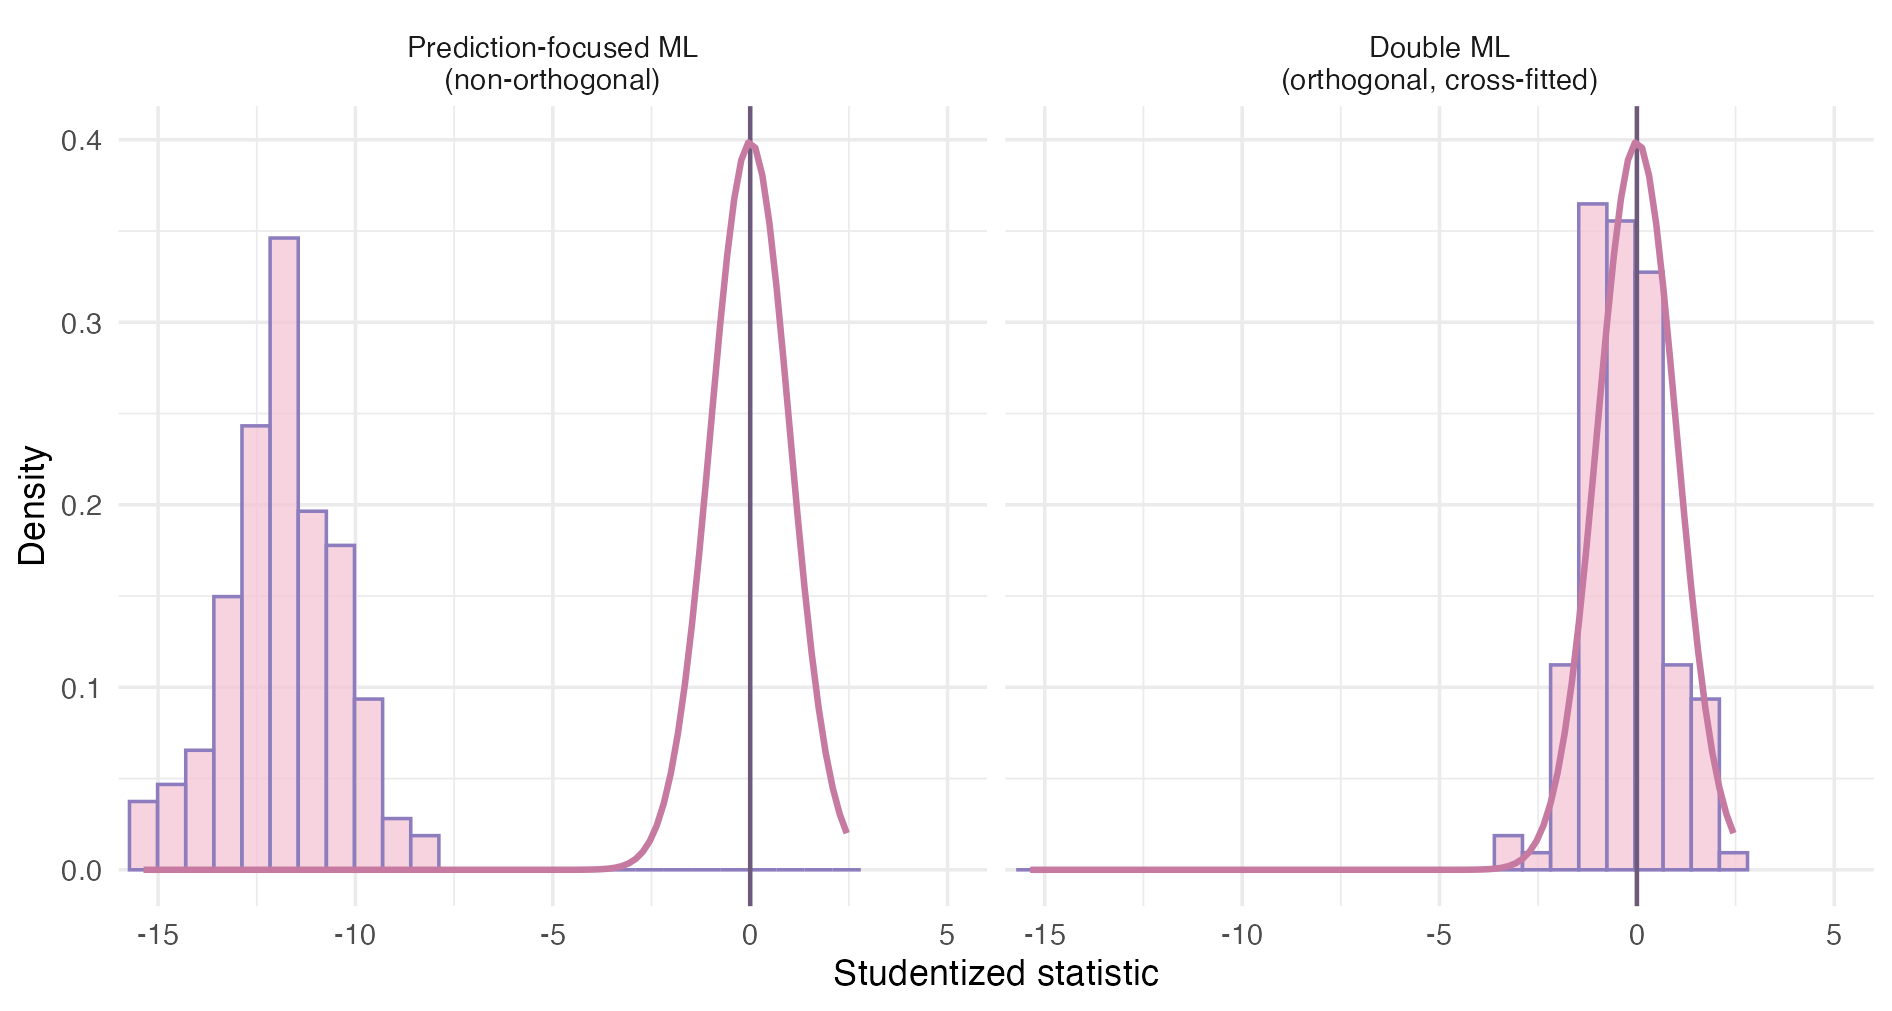
\includegraphics[width=0.94\textwidth]{figures/bias_comparison_life.png}
\caption{Prediction-focused ML versus orthogonal DML in a simulation calibrated to the baseline youth sample. The horizontal axis is the studentized statistic \((\widehat{\beta}-\beta_0)/\widehat{se}\). The non-orthogonal plug-in estimator is poorly centered relative to the \(N(0,1)\) reference curve, whereas the orthogonal cross-fitted estimator is substantially closer to the target distribution.}
\label{fig:bias_comparison_life}
\end{figure}

Figure \ref{fig:bias_comparison_life} illustrates the distinction between an orthogonal and a non-orthogonal estimator using a Monte Carlo design calibrated to the covariate distribution of the baseline youth sample. The observed weekday social-media measure is used as the treatment, while a synthetic outcome is generated from a partially linear model with a known treatment coefficient. The naive estimator uses a prediction model without an orthogonal treatment residual. Its studentized estimates are shifted substantially away from zero. The orthogonal estimator residualizes both treatment and outcome and is evaluated using cross-fitted nuisance predictions, producing a distribution much closer to the \(N(0,1)\) reference curve.\\
\\
\noindent
\textbf{Respondent-level cross-fitting}
\label{sec:cross_fitting_background}\\
\\
Cross-fitting implements the orthogonal score with held-out nuisance predictions. In a \(K\)-fold split, the nuisance learners for fold \(k\) are trained on the other \(K-1\) folds and evaluated only in fold \(k\). Rotating the held-out fold gives out-of-sample estimates of \(\hat\ell\) and \(\hat m\) for every observation. The split can also be repeated \(S\) times with different random folds, with the final estimate of \(\beta\) summarized by the median across repetitions \citep{fuhr2024dml,helal2026returns}. This out-of-sample construction is crucial because orthogonalization alone does not eliminate the dependence created when the same data are used for both training and evaluation \citep{chernozhukov2018dml,bach2024doubleml}.

In this panel, the folds are formed over respondent identifiers, \(I_1,\ldots,I_K\), rather than over person-wave rows. Because the data contain repeated interviews for the same adolescent, all observations belonging to one respondent are assigned to the same fold.\footnote{Keeping each respondent’s observations together in one fold (i.e.\ cross-fitting at the respondent level) prevents leakage across waves and ensures that each adolescent’s nuisance predictions are based on other individuals' data.} For fold \(k\), the nuisance functions \(\widehat{\ell}^{(-k)}(\cdot)\) and \(\widehat{m}^{(-k)}(\cdot)\) are estimated on respondents outside \(I_k\) and evaluated only on the held-out respondents in \(I_k\). The resulting prediction errors are thus evaluated on respondent histories that were not used to train the learner.

In the expansion in Equation \ref{eq:dml_background_decomposition}, the remainder \(R_n\) contains linear nuisance terms such as
\begin{equation}
\left(
\frac{1}{n}\sum_{i,t}V_{it}^{\,2}
\right)^{-1}
\frac{1}{\sqrt{n}}\sum_{i,t}
U_{it}
\left[
m_0(X_{it})
-\widehat{m}^{(-k(i))}(X_{it})
\right]
\label{eq:crossfit_m_remainder}
\end{equation}
and
\begin{equation}
\left(
\frac{1}{n}\sum_{i,t}V_{it}^{\,2}
\right)^{-1}
\frac{1}{\sqrt{n}}\sum_{i,t}
V_{it}
\left[
\ell_0(X_{it})
-\widehat{\ell}^{(-k(i))}(X_{it})
\right].
\label{eq:crossfit_l_remainder}
\end{equation}
Sample splitting makes these terms easier to control because the nuisance estimates are produced from data that are separate from the respondent histories used in the score. Conditional on the training folds, \(\widehat{m}^{(-k)}\) and \(\widehat{\ell}^{(-k)}\) can be treated as fixed functions on fold \(I_k\). For a held-out observation, the law of iterated expectations therefore gives
\begin{equation}
\begin{aligned}
&\mathbb{E}\!\left[
U_{it}
\left\{
m_0(X_{it})-\widehat{m}^{(-k)}(X_{it})
\right\}
\biggm| \mathcal{T}_{-k}
\right] \\
&\quad=
\mathbb{E}\!\left[
\left\{
m_0(X_{it})-\widehat{m}^{(-k)}(X_{it})
\right\}
\mathbb{E}[U_{it}\mid D_{it},X_{it},\mathcal{T}_{-k}]
\biggm| \mathcal{T}_{-k}
\right]
=0,
\end{aligned}
\label{eq:crossfit_m_lie}
\end{equation}
where \(\mathcal{T}_{-k}\) denotes the training data outside fold \(k\). The last equality uses respondent-level separation between the training and evaluation folds together with \(\mathbb{E}[U_{it}\mid D_{it},X_{it}]=0\). The same reasoning applies to the outcome-nuisance term involving \(V_{it}\), using \(\mathbb{E}[V_{it}\mid X_{it}]=0\).

These conditional mean-zero results do not alone prove that the sample sums are \(o_p(1)\); a rate argument is also required. Let \(N_k\) denote the number of respondents in fold \(I_k\), let \(\mathcal{T}_i\) denote the waves observed for respondent \(i\), and suppose that \(T_i=\lvert\mathcal{T}_i\rvert\leq \overline{T}<\infty\). The bounded-cluster assumption is natural here because each adolescent can contribute at most four waves. Consider the fold-specific treatment-nuisance remainder
\begin{equation}
S_{m,k}
=
\frac{1}{\sqrt{N_k}}
\sum_{i\in I_k}
\sum_{t\in\mathcal{T}_i}
U_{it}\Delta^{(-k)}_{m,it},
\qquad
\Delta^{(-k)}_{m,it}
=
m_0(X_{it})-\widehat{m}^{(-k)}(X_{it}).
\label{eq:crossfit_cluster_sum_m}
\end{equation}
Conditional on the training sample \(\mathcal{T}_{-k}\), this sum has mean zero by Equation \ref{eq:crossfit_m_lie}. If respondents are independent across clusters and, for some finite constant \(C_U\),
\begin{equation}
\mathbb{E}[U_{it}^{\,2}\mid D_{it},X_{it}]
\leq C_U<\infty,
\label{eq:bounded_u_second_moment}
\end{equation}
then cross-respondent covariance terms vanish conditional on \(\mathcal{T}_{-k}\). Here \(C_U\) is a uniform upper bound on the conditional second moment of the structural error. For any fold-specific function \(f\), define the held-out fold \(L^2\) norm
\begin{equation*}
\left\|f\right\|_{P_k,2}^{\,2}
:=
\frac{1}{N_k}
\sum_{i\in I_k}
\sum_{t\in\mathcal{T}_i}
\mathbb{E}\!\left[
f(X_{it})^2
\biggm|\mathcal{T}_{-k}
\right],
\end{equation*}
where \(P_k\) denotes the distribution of the held-out respondent histories in fold \(I_k\), conditional on the training sample. Using
\begin{equation*}
\left(\sum_{t\in\mathcal{T}_i}a_{it}\right)^2
\leq
T_i\sum_{t\in\mathcal{T}_i}a_{it}^{\,2}
\leq
\overline{T}\sum_{t\in\mathcal{T}_i}a_{it}^{\,2},
\end{equation*}
the conditional variance satisfies
\begin{equation}
\begin{aligned}
\operatorname{Var}\!\left(S_{m,k}\mid\mathcal{T}_{-k}\right)
&=
\frac{1}{N_k}
\sum_{i\in I_k}
\mathbb{E}\!\left[
\left(
\sum_{t\in\mathcal{T}_i}
U_{it}\Delta^{(-k)}_{m,it}
\right)^2
\biggm|\mathcal{T}_{-k}
\right] \\
&\leq
\frac{\overline{T}}{N_k}
\sum_{i\in I_k}
\sum_{t\in\mathcal{T}_i}
\mathbb{E}\!\left[
U_{it}^{\,2}
\left(\Delta^{(-k)}_{m,it}\right)^2
\biggm|\mathcal{T}_{-k}
\right] \\
&\leq
C_U\overline{T}
\left\|
\widehat{m}^{(-k)}-m_0
\right\|_{P_k,2}^{\,2},
\end{aligned}
\label{eq:crossfit_variance_bound_m}
\end{equation}
Therefore, for every \(\varepsilon>0\), conditional Chebyshev gives
\begin{equation}
\Pr\!\left(
\lvert S_{m,k}\rvert>\varepsilon
\bigm|\mathcal{T}_{-k}
\right)
\leq
\frac{C_U\overline{T}}{\varepsilon^2}
\left\|
\widehat{m}^{(-k)}-m_0
\right\|_{P_k,2}^{\,2}.
\label{eq:crossfit_chebyshev_m}
\end{equation}
If the held-out nuisance prediction is \(L^2\)-consistent, the right-hand side converges to zero in probability. Taking expectations over the training sample gives
\begin{equation}
\Pr\!\left(\lvert S_{m,k}\rvert>\varepsilon\right)
=
\mathbb{E}\!\left[
\Pr\!\left(
\lvert S_{m,k}\rvert>\varepsilon
\bigm|\mathcal{T}_{-k}
\right)
\right]
\longrightarrow 0.
\label{eq:crossfit_unconditional_convergence}
\end{equation}
Thus \(S_{m,k}=o_p(1)\). The corresponding outcome-nuisance remainder is controlled by the same conditional-variance and Chebyshev argument, replacing \(U_{it}\Delta^{(-k)}_{m,it}\) by \(V_{it}\Delta^{(-k)}_{\ell,it}\) and assuming a finite conditional second-moment bound for \(V_{it}\). This is the conditioning step formalized by \citet[Appendix, p.~C50, Lemma~6.1, titled \emph{Conditional convergence implies unconditional}; pp.~C55--C56]{chernozhukov2018dml}, adapted here to independent respondent clusters rather than independent person-wave observations. Because the number of waves per respondent is uniformly bounded, normalization by the number of respondents and normalization by the number of person-wave observations differ only by bounded constants.

Without sample splitting, this conditioning argument is generally unavailable. Let \(\widehat{\ell}\) be estimated on the full sample and let \(\mathcal{T}_n=\sigma(W_1,\ldots,W_n)\) denote all information contained in the observations used to train the learner. The desired step would be
\begin{equation}
\mathbb{E}\!\left[
V_{it}
\left\{
\ell_0(X_{it})-\widehat{\ell}(X_{it})
\right\}
\biggm|\mathcal{T}_n
\right]
=0.
\label{eq:nosplit_desired_mean_zero}
\end{equation}
However, \(\widehat{\ell}(X_{it})\) is now a function of the same \(Y_{it}\) that appears in the evaluation observation, and the maintained restriction \(\mathbb{E}[V_{it}\mid X_{it}]=0\) does not imply \(\mathbb{E}[V_{it}\mid X_{it},\mathcal{T}_n]=0\). In fact,
\begin{equation*}
\mathbb{E}\!\left[
V_{it}
\left\{
\ell_0(X_{it})-\widehat{\ell}(X_{it})
\right\}
\biggm|\mathcal{T}_n
\right]
=
V_{it}
\left\{
\ell_0(X_{it})-\widehat{\ell}(X_{it})
\right\},
\end{equation*}
because the complete in-sample summand is measurable with respect to \(\mathcal{T}_n\). There is no reason for this realized quantity to equal zero. An interpolating learner makes the failure especially transparent. If \(\widehat{\ell}(X_{it})=Y_{it}\) at the training observations, then
\begin{align*}
\ell_0(X_{it})-\widehat{\ell}(X_{it})
&=
\beta_0m_0(X_{it})+g_0(X_{it})
-Y_{it} \\
&=
-\beta_0V_{it}-U_{it},
\end{align*}
and hence
\begin{equation}
\mathbb{E}\!\left[
V_{it}
\left\{
\ell_0(X_{it})-\widehat{\ell}(X_{it})
\right\}
\right]
=
-\beta_0\mathbb{E}[V_{it}^{\,2}]
-\mathbb{E}[V_{it}U_{it}]
=
-\beta_0\mathbb{E}[V_{it}^{\,2}],
\label{eq:nosplit_interpolation_bias}
\end{equation}
which is generally non-zero. The corresponding normalized empirical sum even contains the leading component
\begin{equation*}
-\beta_0
\frac{1}{\sqrt{n}}
\sum_{i,t}V_{it}^{\,2},
\end{equation*}
which need not vanish. This example is not a claim that every in-sample learner fails; it only shows that the conditional mean-zero step cannot be used generically when training and evaluation observations coincide \citep{chernozhukov2018dml}. 

\tocsection{Comparing Linear and DML Estimates}{Comparing linear and DML estimates}
\label{sec:ols_dml_comparison_method}

To compare a linear panel estimate with its DML counterpart, I follow \citet{helal2026returns}. Let \(\widehat{\beta}_{L}\) be the coefficient from the linear model, \(\widehat\beta_{DML,j}\) the corresponding DML coefficient using learner \(j\), and \(\widehat\delta_j = \widehat\beta_L - \widehat\beta_{DML,j}\). Under \(H_0: \delta_j=0\), the \(t\)-statistic
\begin{equation}
t_j
=
\frac{
\widehat{\beta}_{L}-\widehat{\beta}_{DML,j}
}{
\widehat{SE}\!\left(
\widehat{\beta}_{L}-\widehat{\beta}_{DML,j}
\right)
}.
\label{eq:ols_dml_t_test}
\end{equation} is approximately standard normal. Since both coefficients use the same respondents, their difference has variance
\begin{equation}
\begin{aligned}
\mathrm{Var}\!\left(
\widehat{\beta}_{L}-\widehat{\beta}_{DML,j}
\right)
={}&
\mathrm{Var}\!\left(\widehat{\beta}_{L}\right)
+
\mathrm{Var}\!\left(\widehat{\beta}_{DML,j}\right) \\
&-
2\,\mathrm{Cov}\!\left(
\widehat{\beta}_{L},
\widehat{\beta}_{DML,j}
\right).
\end{aligned}
\label{eq:ols_dml_difference_variance}
\end{equation}
I estimate this variance with a paired respondent-level bootstrap, resampling adolescents with all their waves and re-estimating both models. If \(\widehat\delta_j^{*(b)} = \widehat\beta_L^{*(b)} - \widehat\beta_{DML,j}^{*(b)}\) in replication \(b\), the bootstrap standard error is
\begin{equation}
\widehat{SE}_{boot}\!\left(\widehat{\delta}_j\right)
=
\left[
\frac{1}{B-1}
\sum_{b=1}^{B}
\left(
\widehat{\delta}^{*(b)}_j-\overline{\delta}^{*}_j
\right)^2
\right]^{1/2},
\label{eq:ols_dml_bootstrap_se}
\end{equation}
where \(B\) denotes the number of bootstrap replications. The paired procedure preserves the covariance between the two estimates, and I compute the two-sided \(p\)-value as \(p_j = 2[1-\Phi(|t_j|)]\). As noted by \citet{helal2026returns}, this test only checks whether the estimates are statistically distinguishable: non-rejection does not prove equivalence, rejection does not identify the correct model, and DML still cannot remove bias from unobserved confounding.

Chapter \ref{chap:methodology} translates these theoretical elements into the empirical specifications, fold construction, learner choices, and implementation settings.

\bodychapter{Methodology}
\label{chap:methodology}


Building on the empirical setting introduced in Chapters \ref{chap:data} and \ref{chap:theory}, this chapter specifies the econometric models, identification assumptions, and estimation procedures used in the analysis. We first present the linear panel regressions—pooled OLS, fixed effects, and random effects—and then describe the double machine learning (DML) specifications, including the partially linear and interactive models. Finally, we outline the identifying assumptions required for causal interpretation and the estimation strategy for each model. Throughout, all estimation is performed on the youth panel data from UKHLS (Waves \texttt{l}–\texttt{o}) with respondent-clustered standard errors to account for within-adolescent correlation.

\tocsection{Model Specifications}{Model specifications}

\subsection[Linear Regression Models]{Linear regression models}
\label{sec:linear_regression_models}

The analysis first estimates three linear specifications discussed by \citet{ward1993pooled}:
\begin{align*}
MentalHealth_{it}
&=
\alpha
+ \beta SocialMediaUse_{it}
+ X_{it}'\gamma
+ \varepsilon_{it},
&& \text{Pooled OLS}, \\
MentalHealth_{it}
&=
\alpha_i
+ \lambda_t
+ \beta SocialMediaUse_{it}
+ X_{it}'\gamma
+ \varepsilon_{it},
&& \text{Fixed effects}, \\
MentalHealth_{it}
&=
\alpha
+ \beta SocialMediaUse_{it}
+ X_{it}'\gamma
+ u_i
+ \varepsilon_{it},
&& \text{Random effects}.
\end{align*}
For adolescent \(i\) in wave \(t\), \(MentalHealth_{it}\) denotes loneliness, life dissatisfaction, school-work dissatisfaction, or school dissatisfaction. \(SocialMediaUse_{it} \equiv \texttt{ypnetcht}_{it} \in \{1,2,3,4,5\}\) denotes weekday social-media use on the ordered five-category scale. The coefficient \(\beta\) is therefore the estimated change in the outcome associated with a one-category increase in weekday social-media use, conditional on the included controls. Weekend social-media interaction, \(\texttt{ypnetchtw}_{it}\), is measured on the same scale and is used as an alternative treatment in the robustness analysis. The control vector \(X_{it}\) is grouped as
\begin{equation*}
X_{it} = \bigl(X^{\text{demo}}_{it}, X^{\text{geo}}_{it}, X^{\text{hh}}_{it}, X^{\text{social}}_{it}, X^{\text{device}}_{it}\bigr),
\end{equation*}
where \(X^{\text{demo}}_{it}\) contains age, sex, and broad ethnicity; \(X^{\text{geo}}_{it}\) contains urban residence and region; \(X^{\text{hh}}_{it}\) contains household-composition counts for parent figures, grandparents, and siblings; \(X^{\text{social}}_{it}\) contains the number of close friends, family-meal frequency, and television/video time; and \(X^{\text{device}}_{it}\) contains the device-ownership indicators. The common intercept is denoted by \(\alpha\), \(\alpha_i\) is an adolescent-specific intercept, \(\lambda_t\) denotes wave fixed effects, \(u_i\) is the adolescent-specific random effect, and \(\varepsilon_{it}\) is the idiosyncratic error.

The empirical comparison also reports bivariate and basic pooled specifications with smaller control sets, as well as individual fixed effects with and without time fixed effects. All models use respondent-clustered standard errors.

\subsection[Partially Linear Regression Model]{Partially linear regression model}

The first DML specification applies the partially linear framework from Section \ref{sec:dml_background} to the same ordered treatment and control set as the linear models:
\begin{align*}
MentalHealth_{it} &= \beta_0 SocialMediaUse_{it} + g_0(X_{it}) + U_{it}, \\
SocialMediaUse_{it} &= m_0(X_{it}) + V_{it}.
\end{align*}
Here \(g_0(\cdot)\), \(m_0(\cdot)\), and \(\ell_0(X_{it})=\mathbb{E}[MentalHealth_{it}\mid X_{it}]\) are the nuisance functions defined in Chapter \ref{chap:theory}. The target parameter \(\beta_0\) represents the conditional average effect of a one-category increase in weekday social-media use on the outcome, after flexibly adjusting for covariates. Unlike the linear models, this approach does not impose linear-additive restrictions on how controls enter the outcome or the treatment equation \citep{robinson1988rootn,chernozhukov2018dml}. 

\subsection[Interactive Regression Model]{Interactive regression model}

The second DML specification is an interactive (binary-treatment) model that allows heterogeneous treatment effects. We define a binary ``high-use'' indicator: \begin{equation*}
HighUse_{it} = \mathbf{1}\!\left\{SocialMediaUse_{it} \geq 4\right\},
\end{equation*}
which equals one if the adolescent reports at least four hours of weekday social-media use, and zero otherwise. The model is
\begin{align*}
MentalHealth_{it} &= g_0(HighUse_{it}, X_{it}) + U_{it}, \\
HighUse_{it} &= m_0(X_{it}) + V_{it}.
\end{align*} Unlike the partially linear model, this specification does not impose one common treatment coefficient. Instead, the effect of high social-media use is allowed to differ flexibly with the observed covariates through \(g_0(\cdot)\). The target parameter is the average treatment effect,
\begin{equation*}
\theta_0^{ATE} = \mathbb{E}\!\left[g_0(1, X_{it}) - g_0(0, X_{it})\right],
\end{equation*}
which compares high-use and lower-use adolescents after adjusting for covariates in a flexible way. The interactive regression model therefore estimates a high-use contrast rather than a one-category marginal effect \citep{chernozhukov2018dml}.

\subsection[Identification Assumptions]{Identification assumptions}

Both DML models rely on conditional independence: after conditioning on the observed controls \(X_{it}\), the remaining variation in social-media use must be mean-independent of potential outcomes,
\(\mathbb{E}[U_{it}\mid D_{it},X_{it}]=0\),
where \(D_{it}=SocialMediaUse_{it}\) in the partially linear model and \(D_{it}=HighUse_{it}\) in the interactive model. This requires that all confounders of the \(D\)--\(Y\) relationship are captured by \(X_{it}\).\footnote{Unobserved confounders, i.e. variables that affect both social-media use and mental well-being but are not included in \(X_{it}\), would violate conditional independence and remain a limitation of this observational study.} Overlap additionally requires positive treatment probability given \(X_{it}\); for the binary \(HighUse_{it}\), \(0 < \mathbb{P}(HighUse_{it}=1\mid X_{it}) < 1\). It is assessed empirically from the data \citep{chernozhukov2018dml}.

\tocsection{DML Estimation and Implementation}{DML estimation and implementation}

\subsection[The DML Algorithm]{The DML algorithm}

Both DML specifications are estimated on the pooled unbalanced panel from Chapter \ref{chap:data}. The theoretical role of orthogonalization and cross-fitting was detailed in Chapter \ref{chap:theory}, and here we describe how those ideas are implemented. Respondents (not individual person-waves) are divided into \(K=5\) folds. Thus, all available observations for adolescent \(i\) are kept together in either the training sample or the held-out sample.  For the partially linear model, the estimation proceeds as follows:
\begin{enumerate}
\item Randomly partition the respondent identifiers into five folds.
\item For each fold \(k\), use the data from respondents not in fold \(k\) to train two nuisance models: one for the conditional outcome mean \[
    \ell_0(X_{it}) = \mathbb{E}[MentalHealth_{it}\mid X_{it}],
  \] 
  and one for the conditional treatment mean 
  \[
    m_0(X_{it}) = \mathbb{E}[SocialMediaUse_{it}\mid X_{it}].
  \]
\item Apply these trained models to the held-out respondents in fold \(k\), and compute the out-of-sample residuals:
\begin{equation*}
\widetilde{Y}_{it}
=
MentalHealth_{it}-\widehat{\ell}^{(-k)}(X_{it}),
\qquad
\widetilde{D}_{it}
=
SocialMediaUse_{it}-\widehat{m}^{(-k)}(X_{it}).
\end{equation*}
\item Repeat steps 2–3 for each fold until every respondent has a held-out prediction. Stack the residuals \(\widetilde{Y}_{it}, \widetilde{D}_{it}\) across all folds.
\item Estimate \(\beta\) by regressing \(\widetilde{Y}_{it}\) on \(\widetilde{D}_{it}\) (with no intercept):
\begin{equation*}
\widehat{\beta}
=
\frac{\sum_{i,t}\widetilde{D}_{it}\widetilde{Y}_{it}}
{\sum_{i,t}\widetilde{D}_{it}^{\,2}}.
\end{equation*}
\end{enumerate}
This procedure means \(\widehat{\beta}\) is identified from the variation in \(SocialMediaUse_{it}\) that remains after adjusting flexibly for \(X_{it}\). Cross-fitting ensures that each residual \((\widetilde{Y}_{it},\widetilde{D}_{it})\) for an observation is obtained from a nuisance model trained on other respondents’ data \citep{chernozhukov2018dml,knaus2021musicdml,bach2024doubleml}.

The interactive regression model uses the same five-fold structure but a different final step. For each fold, the algorithm estimates out-of-sample fits for the outcome functions \(g_0(1,X_{it})\) and \(g_0(0,X_{it})\), as well as the propensity score \(m_0(X_{it}) = \Pr(HighUse_{it}=1\mid X_{it})\). These are combined in the Neyman-orthogonal ATE score:
\begin{align*}
\psi_{it}(\theta,\eta)
={}&
g(1,X_{it})-g(0,X_{it})
+\frac{HighUse_{it}\{MentalHealth_{it}-g(1,X_{it})\}}{m(X_{it})} \nonumber\\
&-\frac{(1-HighUse_{it})\{MentalHealth_{it}-g(0,X_{it})\}}{1-m(X_{it})}
-\theta.
\end{align*}
where \(\eta\) collects the nuisance components. The ATE estimator \(\widehat{\theta}\) solves the sample moment \(\frac{1}{n}\sum \psi_{it}(\theta,\eta)=0\) \citep{chernozhukov2018dml,bach2024doubleml,baiardi2024valueadded}.

\subsection[Learner Families]{Learner families}

The nuisance functions are estimated with several different machine-learning methods. This deliberate variety ensures that the DML treatment estimate is not sensitive to one particular specification of \(g_0\) or \(m_0\); instead, we can compare how the estimate changes when the nuisance model is linear-sparse, tree-based, or nonlinear \citep{chernozhukov2018dml,fuhr2024dml}.

\paragraph{Elastic net and lasso.}
Both methods fit a linear model with coefficient shrinkage. In the \texttt{glmnet}\footnote{\texttt{glmnet} is a widely used high-performance \texttt{R} package for fitting generalized linear models with lasso or elastic-net regularization \citep{friedman2010glmnet}.} formulation, the coefficient vector \(\gamma\) minimizes
\[
  \frac{1}{n}\sum_{j=1}^n L(Y_j, X_j'\gamma)
  + \lambda \Bigl[\alpha\|\gamma\|_1 + \tfrac{1-\alpha}{2}\|\gamma\|_2^2\Bigr],
\]
where \(L(\cdot)\) is the squared-error loss for regression or logistic loss for classification. Lasso sets \(\alpha=1\), imposing an \(L_1\) penalty that can shrink weak predictors' coefficients to exactly zero (performing variable selection). Elastic net uses \(\alpha=0.5\) (a mix of \(L_1\) and \(L_2\) penalties), which tends to keep groups of correlated features together. This is useful here since many controls (e.g.\ household counts, screen habits, wave dummies) are correlated. The penalty parameter \(\lambda\) is chosen by internal cross-validation: the value that minimizes the out-of-sample prediction error on the training data is selected.\footnote{This internal tuning only uses the training folds for each cross-fit step, not the held-out fold. It is separate from the outer 5-fold cross-fitting loop used to generate orthogonal residuals.} For regression nuisances we use linear \(\ell_2\)-loss; for the IRM propensity score we use the analogous logistic loss \citep{tibshirani1996lasso,zou2005elasticnet,friedman2010glmnet}.

\paragraph{Random forest.}
A random forest builds many decision trees on bootstrap samples of the data, each tree splitting on random subsets of predictors. This allows automated detection of thresholds and interactions without prior specification. We use 300 trees, at each split considering \(\lfloor\sqrt{p}\rfloor\) predictors out of \(p\). Each leaf node has at least 5 observations. The forest averages these trees to reduce variance and de-correlate predictions \citep{breiman2001randomforests}. In practice, regression forests predict continuous nuisance functions, and classification forests produce estimated probabilities \(m_0(X_{it})\) for the binary treatment. Random forests typically capture more complex patterns than linear models, though their piecewise-constant nature can make predictions unstable in sparse regions of the covariate space \citep{wright2017ranger}.

\paragraph{Neural network.}
We implement a simple feedforward neural network (single hidden layer). Each hidden unit computes a weighted sum of the inputs, passes it through a nonlinear activation function \(\sigma(\cdot)\), and the output is a linear combination of these units:
\begin{equation*}
\widehat{f}(X)
=
c+\sum_{r=1}^{R}v_r\,\sigma\!\left(a_r+X'w_r\right).
\end{equation*}
This architecture can approximate complex nonlinearities and interactions, but neural nets are sensitive to architecture choices and regularization. For the PLR nuisance models, we therefore use a small network: one hidden layer with 5 units, weight decay \(0.01\), and up to 300 training iterations. This can capture moderate nonlinearities without overfitting. We report PLR results with this learner, but omit it for the IRM binary-treatment nuisance because preliminary propensity estimates were unstable.\footnote{The smaller high-use class made the IRM propensity fit less stable.} \citep{hornik1989universal,venables2002mass,fuhr2024dml}.

\subsection[Implementing the Code]{Implementing the code}
\label{sec:estimation_workflow}

The analysis is implemented in \texttt{R} using the \texttt{DoubleML}, \texttt{mlr3}, and \texttt{mlr3learners} packages \citep{bach2024doubleml,lang2019mlr3}. For each outcome and treatment definition, we construct a common complete-case dataset. Categorical predictors (e.g.\ region, survey wave) are converted to dummy variables via \texttt{model.matrix}. The respondent ID (\texttt{pidp}) is passed to DoubleMLClusterData but is excluded as a predictor, ensuring that clustering is handled properly.

For the ordered (five-category) treatment, we use \texttt{DoubleMLPLR}. Each column of the results table corresponds to one choice of learner family: within a column, we use the same learner type for both the outcome and treatment nuisance models. For the binary high-use treatment, we use \texttt{DoubleMLIRM} with \texttt{score = "ATE"}: here the outcome nuisance is a regression learner and the propensity is a probabilistic classifier from the same family. Both DML objects use \texttt{n\_folds = 5} and \texttt{DoubleMLClusterData}, enforcing the respondent-level split in cross-fitting. We fix the random seed for each learner to make sample splits and stochastic training reproducible.

By default, we report each DML estimate from one five-fold partition (not an average over multiple splits). For the penalized learners, \(\lambda\) is chosen by the internal cross-validated procedure in \texttt{glmnet}. The random-forest and neural-network hyperparameters are as described above. All reported standard errors are clustered by respondent, and conventional significance levels are shown.

To compare fixed-effects and DML estimates, we use a paired respondent-cluster bootstrap (Section \ref{sec:ols_dml_comparison_method}) with \(B=500\) replications. In each bootstrap sample, we resample respondents with replacement (keeping all their waves together) and re-estimate both the fixed-effects model and the DML model on that sample, preserving their clustering. This captures the covariance between the two estimators when computing the test statistic.

The implemented workflow follows the architecture outlined by \citet{bach2024doubleml}. Internally, \texttt{DoubleMLPLR} and \texttt{DoubleMLIRM} invoke the appropriate learners from the \texttt{mlr3} ecosystem, which in turn rely on \texttt{glmnet}, \texttt{ranger}, and \texttt{nnet} for the learner-specific computation \citep{friedman2010glmnet,wright2017ranger,venables2002mass}.

Finally, to facilitate reproducibility, the replication repository is available at \url{https://github.com/mvdberg1/msc-thesis-dml-social-media-mental-health}. It includes a \texttt{REPLICATION.md} file documenting the restricted UKHLS data source, required directory structure, software dependencies, script order, random seeds, and commands needed to reproduce the results. Because the raw UKHLS data cannot be redistributed, replication requires users to provide their own licensed copy.

With the data, estimands, identifying assumptions, and estimation procedure now fully specified, Chapter \ref{chap:res} presents the empirical findings.

\tocchapter{Empirical Analysis}{Empirical analysis}
\label{chap:res}

\tocsection{Linear Panel-Data Model Results}{Linear panel-data model results}

\subsection[Linear Model Estimates]{Linear model estimates}

This section first reports the linear panel-data results. Table \ref{tab:pooled_ols_life} focuses on life dissatisfaction, which is the broadest of the wellbeing outcomes. Column (1) is a bivariate pooled OLS model. Column (2) adds a small set of basic controls from Table \ref{tab:descriptive_statistics}, namely age, female, and urban area. Column (3) estimates the rich pooled linear model. Columns (4) and (5) move to fixed-effects specifications with rich controls, first without and then with wave fixed effects.\footnote{The female indicator is time-invariant within respondents and is therefore absorbed by the individual fixed effects rather than estimated as a separate coefficient.} Column (6) reports the random-effects model with rich controls. The control rows follow the main variables in Table \ref{tab:descriptive_statistics}. All coefficients are estimated on a common outcome-specific sample and use respondent-clustered standard errors. Since higher values indicate worse wellbeing, positive coefficients imply more life dissatisfaction as weekday social-media use increases. Appendix Tables \ref{tab:linear_models_loneliness}, \ref{tab:linear_models_schoolwork}, and \ref{tab:linear_models_school} report the same six-column sequence for the other three wellbeing outcomes.

\begin{table}[!htbp]
\centering
\caption{Linear model estimates for life dissatisfaction}
\label{tab:pooled_ols_life}
\scriptsize
\setlength{\tabcolsep}{3.2pt}
\renewcommand{\arraystretch}{0.9}
\begin{tabular}{p{0.34\textwidth}cccccc}
\hline
Variable & (1) & (2) & (3) & (4) & (5) & (6) \\
\hline
Weekday social-media use & \shortstack[c]{0.172*** \\[-0.35ex] (0.029)} & \shortstack[c]{0.143*** \\[-0.35ex] (0.028)} & \shortstack[c]{0.056* \\[-0.35ex] (0.029)} & \shortstack[c]{0.032 \\[-0.35ex] (0.041)} & \shortstack[c]{0.030 \\[-0.35ex] (0.041)} & \shortstack[c]{0.056** \\[-0.35ex] (0.027)}
\\
Age &  & \shortstack[c]{0.120*** \\[-0.35ex] (0.013)} & \shortstack[c]{0.097*** \\[-0.35ex] (0.013)} & \shortstack[c]{0.123*** \\[-0.35ex] (0.024)} & \shortstack[c]{-0.004 \\[-0.35ex] (0.139)} & \shortstack[c]{0.101*** \\[-0.35ex] (0.012)}
\\
Female &  & \shortstack[c]{0.424*** \\[-0.35ex] (0.046)} & \shortstack[c]{0.385*** \\[-0.35ex] (0.049)} &  &  & \shortstack[c]{0.356*** \\[-0.35ex] (0.047)}
\\
Urban area &  & \shortstack[c]{-0.088 \\[-0.35ex] (0.057)} & \shortstack[c]{-0.142** \\[-0.35ex] (0.059)} & \shortstack[c]{-0.189 \\[-0.35ex] (0.310)} & \shortstack[c]{-0.216 \\[-0.35ex] (0.312)} & \shortstack[c]{-0.143*** \\[-0.35ex] (0.055)}
\\
Close friends &  &  & \shortstack[c]{-0.312*** \\[-0.35ex] (0.035)} & \shortstack[c]{-0.264*** \\[-0.35ex] (0.052)} & \shortstack[c]{-0.265*** \\[-0.35ex] (0.052)} & \shortstack[c]{-0.301*** \\[-0.35ex] (0.033)}
\\
Parents/step-parents in household &  &  & \shortstack[c]{-0.114** \\[-0.35ex] (0.057)} & \shortstack[c]{-0.030 \\[-0.35ex] (0.123)} & \shortstack[c]{-0.030 \\[-0.35ex] (0.123)} & \shortstack[c]{-0.103* \\[-0.35ex] (0.053)}
\\
Grandparents in household &  &  & \shortstack[c]{-0.049 \\[-0.35ex] (0.083)} & \shortstack[c]{0.581 \\[-0.35ex] (0.432)} & \shortstack[c]{0.586 \\[-0.35ex] (0.434)} & \shortstack[c]{-0.009 \\[-0.35ex] (0.086)}
\\
Siblings/step-siblings in household &  &  & \shortstack[c]{-0.007 \\[-0.35ex] (0.025)} & \shortstack[c]{0.025 \\[-0.35ex] (0.149)} & \shortstack[c]{0.032 \\[-0.35ex] (0.150)} & \shortstack[c]{0.006 \\[-0.35ex] (0.023)}
\\
Family meals &  &  & \shortstack[c]{-0.178*** \\[-0.35ex] (0.023)} & \shortstack[c]{-0.089** \\[-0.35ex] (0.045)} & \shortstack[c]{-0.086* \\[-0.35ex] (0.045)} & \shortstack[c]{-0.168*** \\[-0.35ex] (0.022)}
\\
Television/video hours &  &  & \shortstack[c]{0.201*** \\[-0.35ex] (0.034)} & \shortstack[c]{0.071 \\[-0.35ex] (0.048)} & \shortstack[c]{0.071 \\[-0.35ex] (0.048)} & \shortstack[c]{0.165*** \\[-0.35ex] (0.031)}
\\
Smartphone &  &  & \shortstack[c]{-0.148** \\[-0.35ex] (0.070)} & \shortstack[c]{-0.071 \\[-0.35ex] (0.092)} & \shortstack[c]{-0.071 \\[-0.35ex] (0.092)} & \shortstack[c]{-0.112* \\[-0.35ex] (0.064)}
\\
Tablet &  &  & \shortstack[c]{-0.026 \\[-0.35ex] (0.044)} & \shortstack[c]{0.081 \\[-0.35ex] (0.067)} & \shortstack[c]{0.081 \\[-0.35ex] (0.068)} & \shortstack[c]{-0.009 \\[-0.35ex] (0.040)}
\\
Gaming console &  &  & \shortstack[c]{0.049 \\[-0.35ex] (0.054)} & \shortstack[c]{-0.027 \\[-0.35ex] (0.081)} & \shortstack[c]{-0.030 \\[-0.35ex] (0.081)} & \shortstack[c]{0.025 \\[-0.35ex] (0.049)}
\\
Laptop/desktop computer &  &  & \shortstack[c]{-0.003 \\[-0.35ex] (0.055)} & \shortstack[c]{-0.142* \\[-0.35ex] (0.080)} & \shortstack[c]{-0.139* \\[-0.35ex] (0.080)} & \shortstack[c]{-0.028 \\[-0.35ex] (0.050)}
\\
\hline
Model & Bivariate & Basic & Rich pooled & FE & FE + wave & RE
\\
$R^2$ & 0.012 & 0.062 & 0.134 & 0.055 & 0.056 & 0.148
\\
N & 4,316 & 4,316 & 4,316 & 4,316 & 4,316 & 4,316
\\
\hline
\end{tabular}
\renewcommand{\arraystretch}{1}
\begin{minipage}{0.97\textwidth}
\footnotesize Notes: All columns use the same common outcome-specific sample and report respondent-clustered standard errors in parentheses below the coefficient. Column (1) is a bivariate pooled OLS model. Column (2) adds age, female, and urban-area controls. Column (3) adds the rich baseline control set in a standard pooled linear regression. Column (4) is a fixed-effects model with rich controls and individual intercepts. Column (5) adds wave fixed effects to the fixed-effects model. Column (6) is a random-effects model with rich controls. Blank cells indicate covariates that are absorbed by individual fixed effects or otherwise not identified in a given specification. The rich-control models also include broad ethnicity and region dummies, which are omitted from display for compactness. The row labeled Close friends refers to the logged control \texttt{log(1 + close\_friends)} used in the regressions. Significance: *** \(p < 0.01\), ** \(p < 0.05\), * \(p < 0.10\).
\end{minipage}
\end{table}


The life-dissatisfaction results show a clear attenuation pattern. The bivariate coefficient is \(0.172\), it falls to \(0.143\) once the basic controls are added, and it drops further to \(0.056\) in the rich pooled OLS specification. Once individual fixed effects are introduced, the coefficient becomes much smaller, at about \(0.032\) without wave effects and \(0.030\) with wave effects, and it is no longer statistically different from zero. The random-effects estimate, by contrast, remains at \(0.056\), much closer to the rich pooled OLS result than to the fixed-effects coefficients. This suggests that observable differences explain part of the raw association, but that respondent-specific time-invariant heterogeneity explains an additional part once the comparison is shifted to within-adolescent changes over time. Among the controls, more close friends and more frequent family meals are associated with lower life dissatisfaction, while more television/video time is associated with higher life dissatisfaction.

\subsection[Panel-Model Specification Tests]{Panel-model specification tests}

Table \ref{tab:panel_model_tests} reports the three standard panel-model specification tests alongside the weekday social-media coefficients from the linear specifications in Table \ref{tab:pooled_ols_life} and its appendix counterparts, specifically columns (3), (5), and (6).

\begin{table}[!htbp]
\centering
\caption{Panel-model comparison and specification tests}
\label{tab:panel_model_tests}
\scriptsize
\resizebox{\textwidth}{!}{%
\begin{tabular}{lcccc}
\hline
Model or test & Life dissatisfaction & Loneliness & School-work dissatisfaction & School dissatisfaction
\\
\hline
Pooled classical linear regression model & 0.056* (0.029) & 0.022* (0.013) & 0.116*** (0.033) & 0.071** (0.035)
\\
Fixed effects model & 0.030 (0.041) & 0.042** (0.020) & 0.051 (0.045) & 0.013 (0.050)
\\
Random effects model & 0.056** (0.027) & 0.030** (0.012) & 0.103*** (0.031) & 0.060* (0.033)
\\
F test p-value & $< 0.001$ & $< 0.001$ & $< 0.001$ & $< 0.001$
\\
LM test p-value & $< 0.001$ & $< 0.001$ & $< 0.001$ & $< 0.001$
\\
Hausman p-value & 0.046 & $< 0.001$ & $< 0.001$ & $< 0.001$
\\
N & 4,316 & 4,298 & 4,329 & 4,316
\\
\hline
\end{tabular}
}
\begin{minipage}{0.95\textwidth}
\footnotesize Notes: The first three rows reproduce the weekday social-media coefficient from the outcome-specific linear-results tables, specifically columns (3), (5), and (6). All rows use the same outcome-specific estimation samples as those tables. Robust standard errors are clustered at the respondent level. The F test evaluates the pooled-versus-fixed-effects comparison on the matched rich-control specifications without wave dummies. The Breusch-Pagan LM test evaluates the pooled-versus-random-effects comparison for the matched rich-control specifications, using the unbalanced-panel implementation in \texttt{plm}. The Hausman test evaluates the fixed-versus-random-effects comparison on the matched rich-control specifications without wave dummies. Small p-values therefore reject the simpler or stronger-assumption model in favour of the more flexible alternative. Significance: *** \(p < 0.01\), ** \(p < 0.05\), * \(p < 0.10\).
\end{minipage}
\end{table}


Table \ref{tab:panel_model_tests} shows that the fixed-effects coefficients are generally smaller than the pooled and random-effects coefficients, especially for the dissatisfaction outcomes. This suggests that part of the pooled association reflects stable respondent-specific heterogeneity. Following \citet{ward1993pooled}, Table \ref{tab:pooled_ols_life} and its appendix counterparts also report \(R^2\), but these fit measures are only descriptive here because the fixed-effects \(R^2\) is based on within-respondent transformed variation and is therefore not directly comparable to the pooled and random-effects values.

The model-selection tests are clearer. For all four outcomes, the global F test and the Breusch--Pagan LM test give \(p < 0.001\), so pooled classical linear regression is rejected against both fixed effects and random effects. Because social-media use is observational rather than randomly assigned, the fixed-effects model is substantively plausible, and the Hausman test points in the same direction: \(p = 0.046\) for life dissatisfaction and \(p < 0.001\) for loneliness, school-work dissatisfaction, and school dissatisfaction. The fixed-effects model is therefore preferred in all four cases and serves as the main linear panel model in the subsequent comparison.

\tocsection{Double Machine Learning Results}{Double machine learning results}

\subsection[Partially Linear Double Machine Learning]{Partially linear double machine learning}

Table \ref{tab:dml_life_methods} then reports the partially linear double machine learning estimate for life dissatisfaction across alternative nuisance learners. All columns use the same pooled Waves \texttt{l}--\texttt{o} sample, the same rich control set, and wave effects inside the control vector.

\begin{table}[!htbp]
\centering
\caption{Partially linear double machine learning estimates for life dissatisfaction across nuisance learners}
\label{tab:dml_life_methods}
\begin{tabular}{lcccc}
\hline
Variable & Elastic net & Lasso & Random forest & Neural net
\\
\hline
Weekday social-media use & 0.057* & 0.062** & 0.056* & 0.029
\\
 & (0.029) & (0.029) & (0.029) & (0.029)
\\
N & 4,316 & 4,316 & 4,316 & 4,316
\\
\hline
\end{tabular}
\begin{minipage}{0.95\textwidth}
\footnotesize Notes: All columns report pooled double machine learning estimates from the partially linear regression specification for the coefficient on weekday social-media use. The same common outcome-specific sample with rich controls is used throughout, and wave fixed effects are included among the controls. Elastic net uses alpha = 0.5, while Lasso uses alpha = 1. Standard errors come from respondent-clustered DoubleML inference with 5-fold cross-fitting. Significance: *** \(p < 0.01\), ** \(p < 0.05\), * \(p < 0.10\).
\end{minipage}
\end{table}


The partially linear double machine learning results are reassuringly stable. The estimated coefficient on weekday social-media use remains positive across all four learners and lies between about \(0.029\) and \(0.062\). The elastic-net, lasso, and random-forest estimates are all very close to the rich pooled OLS coefficient from Table \ref{tab:pooled_ols_life}, while the neural-net estimate is smaller and less precise. Appendix Tables \ref{tab:dml_loneliness_methods}, \ref{tab:dml_schoolwork_methods}, and \ref{tab:dml_school_methods} report the same partially linear comparison for the other three wellbeing outcomes. Taken together, these results suggest that allowing more flexible nuisance functions does not overturn the basic conclusion from the linear models: the raw association shrinks substantially once confounding is handled more carefully, but it does not disappear entirely in the pooled specifications.

The magnitude is modest relative to the observed dispersion of life dissatisfaction. For example, a coefficient of \(0.056\) corresponds to about \(0.044\) of the recent-wave outcome standard deviation of \(1.28\) for a one-category increase in weekday use. If the linear specification is extrapolated across the full four-category contrast from no use to seven or more hours, the implied difference is \(0.224\) points, or about \(0.175\) standard deviations. This calculation is a scale interpretation rather than a causal effect or a dose-response estimate: the treatment consists of broad ordered categories, and the extrapolation imposes the constant-slope restriction of the PLR model.

\subsection[Interactive Regression Model Double Machine Learning]{Interactive regression model double machine learning}

Table \ref{tab:irm_life_methods} complements this by switching from the ordered weekday-use scale to the binary high-use indicator and estimating an interactive regression model average treatment effect with double machine learning. This changes the estimand: the coefficients now compare adolescents with at least four hours of weekday social-media use to the rest of the sample, conditional on the same rich control set and wave effects.

\begin{table}[!htbp]
\centering
\caption{Interactive regression model double machine learning estimates for life dissatisfaction across nuisance learners}
\label{tab:irm_life_methods}
\begin{tabular}{lccc}
\hline
Variable & Elastic net & Lasso & Random forest
\\
\hline
High social-media use & 0.168 & 0.224 & -0.017
\\
 & (0.121) & (0.138) & (0.205)
\\
N & 4,316 & 4,316 & 4,316
\\
\hline
\end{tabular}
\begin{minipage}{0.95\textwidth}
\footnotesize Notes: All columns report pooled double machine learning average treatment effect estimates from the interactive regression model for the binary indicator of at least four hours of weekday social-media use. The same common outcome-specific sample with rich controls is used throughout, and wave fixed effects are included among the controls. Elastic net uses alpha = 0.5, while Lasso uses alpha = 1 for both the outcome and propensity nuisances. The interactive-regression comparison is restricted to Elastic net, Lasso, and Random forest because these were the learners that remained numerically stable in the binary-treatment setting. Standard errors come from respondent-clustered DoubleML inference with 5-fold cross-fitting. Significance: *** \(p < 0.01\), ** \(p < 0.05\), * \(p < 0.10\).
\end{minipage}
\end{table}


The interactive regression model estimates are more sensitive to learner choice than the partially linear estimates. For life dissatisfaction, the elastic-net and lasso specifications remain positive, whereas the random-forest estimate is close to zero and slightly negative. This suggests that the binary high-use contrast is less stable in this application than the ordered-treatment partially linear specification, which is plausible given that the high-use group is much smaller than the full five-category treatment distribution. Appendix Tables \ref{tab:irm_loneliness_methods}, \ref{tab:irm_schoolwork_methods}, and \ref{tab:irm_school_methods} report the corresponding interactive-regression comparisons for the other three wellbeing outcomes.

\tocsection{Comparison Between Fixed-Effects and DML Estimates}{Comparison between fixed-effects and DML estimates}

The final comparison asks whether the preferred fixed-effects estimates and the corresponding DML estimates for life dissatisfaction differ statistically. Table \ref{tab:fe_dml_comparison} separates two comparisons because the partially linear and interactive-regression models use different treatment definitions. Panel A compares the fixed-effects coefficient on the ordered five-category weekday-use measure with the four PLR-DML estimates from Table \ref{tab:dml_life_methods}. Panel B compares the IRM-DML estimates from Table \ref{tab:irm_life_methods} with a separately estimated fixed-effects model that uses the same binary high-use indicator. This prevents differences in treatment scale from being attributed incorrectly to the estimation method.

Section \ref{sec:ols_dml_comparison_method} introduced the paired comparison, following \citet{helal2026returns}. Here both the relevant fixed-effects estimator and each DML estimator are re-estimated in every respondent-cluster bootstrap sample. The resulting standard error of the difference therefore incorporates their sampling covariance.

\begin{table}[!htbp]
\centering
\caption{Paired comparisons of fixed-effects and DML estimates for life dissatisfaction}
\label{tab:fe_dml_comparison}
\small
\setlength{\tabcolsep}{6pt}
\begin{tabular}{lcccc}
\hline
Statistic & Elastic net & Lasso & Random forest & Neural net
\\
\hline
\multicolumn{5}{l}{\textit{Panel A: Ordered-treatment FE versus PLR-DML}} \\
$t$-statistic & -0.656 & -0.781 & -0.570 & 0.030
\\
$p$-value & 0.512 & 0.435 & 0.568 & 0.976
\\[0.4ex]
\multicolumn{5}{l}{\textit{Panel B: Binary-treatment FE versus IRM-DML}} \\
$t$-statistic & -0.898 & -1.229 & 0.319 & --
\\
$p$-value & 0.369 & 0.219 & 0.750 & --
\\
\hline
\end{tabular}
\begin{minipage}{0.96\textwidth}
\footnotesize Notes: Panel A compares the fixed-effects coefficient on the ordered five-category weekday-use measure with the PLR-DML coefficients in Table~\ref{tab:dml_life_methods}. Panel B compares a separately estimated fixed-effects coefficient on the binary high-use indicator with the IRM-DML average treatment effects in Table~\ref{tab:irm_life_methods}. The neural-net IRM cell is not reported because that learner was not retained in the binary-treatment analysis. For both panels, standard errors of the paired differences use 500 respondent-cluster bootstrap replications, and the two-sided $p$-values use the standard-normal approximation. All comparisons use the same outcome-specific sample with $N=4,316$ person-wave observations.
\end{minipage}
\end{table}


Panel A shows that none of the PLR-DML estimates differs statistically from the preferred ordered-treatment fixed-effects estimate. The fixed-effects coefficient is \(0.030\). The elastic-net, lasso, and random-forest DML estimates are somewhat larger, at \(0.057\), \(0.062\), and \(0.056\), giving FE-minus-DML differences between \(-0.025\) and \(-0.031\). Their paired test statistics range from \(-0.570\) to \(-0.781\), with \(p\)-values between \(0.435\) and \(0.568\). The neural-net estimate, \(0.029\), is almost identical to the fixed-effects estimate and gives a \(p\)-value of \(0.976\).

Panel B leads to the same inferential conclusion for the binary high-use treatment. The corresponding fixed-effects coefficient is \(0.036\), compared with IRM-DML estimates of \(0.168\), \(0.224\), and \(-0.017\) for elastic net, lasso, and random forest. The paired \(t\)-statistics are \(-0.898\), \(-1.229\), and \(0.319\), with \(p\)-values of \(0.369\), \(0.219\), and \(0.750\), respectively. Thus, the null of equal estimates is not rejected for either treatment definition or any learner, even at the 10 percent level.

Appendix Tables \ref{tab:fe_dml_comparison_loneliness}, \ref{tab:fe_dml_comparison_schoolwork_dissatisfaction}, and \ref{tab:fe_dml_comparison_school_dissatisfaction} extend these paired tests to the other outcomes. None of the ordered-treatment PLR-DML estimates differs significantly from its fixed-effects counterpart, and the binary-treatment estimates for loneliness likewise show no significant differences. The IRM comparison is less stable for the school outcomes. For school-work dissatisfaction, the IRM-DML estimate differs significantly from the binary fixed-effects estimate for elastic net (\(p=0.007\)), lasso (\(p=0.003\)), and random forest (\(p=0.008\)). For school dissatisfaction, only the random-forest difference is significant (\(p=0.019\)); the elastic-net and lasso differences are not. Because these appendix comparisons span several outcomes and learners, the individual rejections should be treated as exploratory: no family-wise or false-discovery-rate adjustment was prespecified.

For the ordered treatment, the numerical gaps between the fixed-effects and PLR-DML estimates are small relative to their joint sampling uncertainty across all outcomes. This provides a relatively consistent robustness result for flexible nuisance estimation. The binary-treatment evidence is more qualified because the IRM differences for the school outcomes are sometimes statistically significant. None of these tests establishes statistical equivalence, nor do they remove the difference in identifying variation and functional form between the models: fixed effects use within-adolescent changes, whereas pooled DML flexibly adjusts for observed covariates. The fixed-effects attenuation therefore remains relevant when interpreting the larger pooled DML point estimates.

\tocsection{Robustness Checks}{Robustness checks}
\label{sec:robustness_results}

The robustness checks retain life dissatisfaction as the outcome and examine whether the main findings depend on the exposure definition, wave coverage, control set, cross-fitting partition, propensity-score support, or the selection-on-observables assumption. These checks alter different assumptions rather than forming a single ranking of estimators. Fixed effects are less reliant than pooled specifications on the absence of stable unobserved respondent heterogeneity, but require informative within-person treatment changes. PLR-DML relaxes functional-form restrictions on observed-confounder adjustment while retaining the selection-on-observables assumption. For the binary treatment, IRM-DML also permits treatment-effect heterogeneity, but places greater demands on propensity-score overlap. The design of each check is introduced alongside its results below.

\subsection[Alternative Exposure, Wave Coverage, and Control Sets]{Alternative exposure, wave coverage, and control sets}

Table \ref{tab:robustness_weekend} first replaces weekday use with weekend social-media use and re-estimates the models on the full weekend complete-case sample. Panel A uses the ordered five-category weekend measure and compares fixed effects with PLR-DML. Panel B defines high weekend use as at least four hours and compares a corresponding binary fixed-effects model with IRM-DML. Standard errors are displayed below the coefficients to keep the two comparisons readable. The Panel A equality tests use the paired respondent-cluster bootstrap introduced in Section \ref{sec:ols_dml_comparison_method}, with both estimators re-estimated in each of 500 samples. Panel B uses 500 paired respondent-cluster influence-function bootstrap draws.\footnote{The same respondent-cluster weights are applied to the estimated FE and IRM influence contributions in each draw, thereby retaining the sampling covariance between the two estimators.}

\begin{table}[!htbp]
\centering
\caption{Weekend social-media use and paired fixed-effects--DML comparisons}
\label{tab:robustness_weekend}
\small
\setlength{\tabcolsep}{5pt}
\begin{tabular*}{\textwidth}{@{\extracolsep{\fill}}lccccc}
\hline
Statistic & Fixed effects & Elastic net & Lasso & Random forest & Neural net
\\
\hline
\multicolumn{6}{l}{\textit{Panel A: Ordered-treatment FE versus PLR-DML}} \\
Weekend-use estimate & -0.011 & 0.025 & 0.025 & 0.023 & 0.032
\\
 & (0.034) & (0.024) & (0.024) & (0.024) & (0.023)
\\
$t$-statistic & -- & -1.038 & -1.026 & -0.953 & -1.214
\\
$p$-value & -- & 0.299 & 0.305 & 0.341 & 0.225
\\[0.5ex]
\multicolumn{6}{l}{\textit{Panel B: Binary-treatment FE versus IRM-DML}} \\
High weekend use estimate & 0.060 & 0.078* & 0.073 & 0.082* & --
\\
 & (0.057) & (0.046) & (0.045) & (0.047) & --
\\
$t$-statistic & -- & -0.283 & -0.201 & -0.333 & --
\\
$p$-value & -- & 0.777 & 0.841 & 0.739 & --
\\
\hline
\end{tabular*}
\begin{minipage}{0.97\textwidth}
\footnotesize Notes: Standard errors are reported in parentheses below the coefficients. Panel A uses the ordered five-category weekend-use measure. Panel B defines high weekend use as at least four hours and reports the IRM average treatment effect. The fixed-effects models include respondent and wave effects; DML uses five-fold respondent-level cross-fitting. The neural-net IRM is not reported. Panel A uses 500 full respondent-cluster bootstrap re-estimations. Panel B uses 500 paired respondent-cluster influence-function bootstrap draws. The complete-case sample contains $N=4,331$ person-wave observations. $^{***}p<0.01$, $^{**}p<0.05$, $^{*}p<0.10$.
\end{minipage}
\end{table}


The ordered weekend coefficients are small and individually imprecise across all specifications. The fixed-effects estimate is \(-0.011\), while the PLR-DML estimates range from \(0.023\) to \(0.032\). None of these differences is statistically significant: the paired \(t\)-statistics range from \(-0.953\) to \(-1.214\), with \(p\)-values between \(0.225\) and \(0.341\). The binary weekend estimates are positive, at \(0.060\) for fixed effects and between \(0.073\) and \(0.082\) for IRM-DML, but their paired differences are also far from significant, with \(p\)-values between \(0.739\) and \(0.841\). The alternative exposure therefore does not produce evidence that the weekend FE and DML estimators differ. Moreover, the absence of a precisely estimated ordered weekend coefficient shows that the positive weekday association does not generalize directly to the five-category weekend measure.

Table \ref{tab:robustness_extended_waves} then separates control-set sensitivity from wave coverage and adds paired comparisons for the all-wave specification. Extending the sample from Waves \texttt{l}--\texttt{o} to all youth Waves \texttt{a}--\texttt{o} makes it impossible to retain the six device-access indicators used in the rich baseline specification. The longer panel therefore uses a common-core set of eleven demographic, geographic, household, social-environment, family-meal, and television-use controls that are available throughout all fifteen waves.\footnote{The availability audit identifies 17 candidate variables that are jointly available from Waves \texttt{a}--\texttt{o}. This count includes the treatment and several alternative outcomes and therefore does not represent 17 control variables.} Panel A first reports the rich recent-wave baseline, then applies the common-core controls to the same Waves \texttt{l}--\texttt{o}, and finally changes only the wave coverage by applying that specification to Waves \texttt{a}--\texttt{o}. Panel B reports the corresponding binary high-use FE and IRM-DML estimates for Waves \texttt{a}--\texttt{o}. For both all-wave comparisons, 500 paired respondent-cluster influence-function bootstrap draws are used to estimate the standard error of the FE--DML difference.

\begin{table}[!htbp]
\centering
\caption{Wave coverage, controls, and paired all-wave DML comparisons}
\label{tab:robustness_extended_waves}
\small
\setlength{\tabcolsep}{5pt}
\begin{tabular*}{\textwidth}{@{\extracolsep{\fill}}lccccc}
\hline
Specification & Fixed effects & Elastic net & Lasso & Random forest & Neural net
\\
\hline
\multicolumn{6}{l}{\textit{Panel A: Ordered-treatment FE versus PLR-DML}} \\
Waves l--o, rich controls & 0.030 & 0.057* & 0.062** & 0.056* & 0.029
\\
 & (0.041) & (0.029) & (0.029) & (0.029) & (0.029)
\\
Waves l--o, common-core controls & 0.035 & 0.065** & 0.068** & 0.054** & 0.053*
\\
 & (0.036) & (0.027) & (0.028) & (0.027) & (0.028)
\\
Waves a--o, common-core controls & 0.079*** & 0.116*** & 0.115*** & 0.112*** & 0.107***
\\
 & (0.011) & (0.009) & (0.009) & (0.009) & (0.009)
\\
$t$-statistic, Waves a--o & -- & -3.728 & -3.651 & -3.285 & -2.753
\\
$p$-value, Waves a--o & -- & $<0.001$ & $<0.001$ & 0.001 & 0.006
\\[0.5ex]
\multicolumn{6}{l}{\textit{Panel B: Binary-treatment FE versus IRM-DML}} \\
Waves a--o, high weekday use & 0.167*** & 0.285*** & 0.289*** & 0.240*** & --
\\
 & (0.025) & (0.032) & (0.032) & (0.040) & --
\\
$t$-statistic & -- & -3.741 & -3.904 & -1.835 & --
\\
$p$-value & -- & $<0.001$ & $<0.001$ & 0.066 & --
\\
\hline
\end{tabular*}
\begin{minipage}{0.97\textwidth}
\footnotesize Notes: Standard errors are reported in parentheses below the coefficients. Panel A preserves the control-set and wave-coverage comparison and reports paired tests for the Waves a--o common-core specification. Panel B uses the same all-wave sample and defines high weekday use as at least four hours. The neural-net IRM is not reported. Standard errors of the paired differences use 500 paired respondent-cluster influence-function bootstrap draws. The Waves l--o rich-control sample contains $N=4,316$, the Waves l--o common-core sample contains $N=5,001$, and the Waves a--o common-core sample contains $N=33,184$ person-wave observations. $^{***}p<0.01$, $^{**}p<0.05$, $^{*}p<0.10$.
\end{minipage}
\end{table}


Removing the device indicators within Waves \texttt{l}--\texttt{o} changes the estimates only modestly. The fixed-effects coefficient moves from \(0.030\) to \(0.035\), and the four DML estimates remain in a narrow positive range between \(0.053\) and \(0.068\). The larger change occurs when the common-core model is extended to all waves. The ordered-treatment fixed-effects estimate rises to \(0.079\), while the PLR-DML estimates range from \(0.107\) to \(0.116\); all are precisely estimated. Unlike the recent-wave results, each all-wave PLR-DML estimate is significantly larger than the fixed-effects estimate, with paired \(p\)-values ranging from below \(0.001\) to \(0.006\). Panel B shows a similar pattern for elastic net and lasso: their IRM estimates of \(0.285\) and \(0.289\) differ significantly from the binary fixed-effects estimate of \(0.167\), both with \(p<0.001\). The random-forest IRM estimate is \(0.240\), and its difference is significant only at the 10 percent level (\(p=0.066\)). The increased precision follows partly from the much larger sample of \(33{,}184\) person-wave observations. The larger point estimates and significant method differences indicate that the relationship is not constant across survey periods or identifying specifications. Consequently, the all-wave result strengthens the evidence for a positive conditional association, but it should not be read as directly interchangeable with the recent-wave baseline effect.

As a further check on wave composition, the baseline specification is re-estimated four times after omitting one recent wave at a time. This produces four explicit subsample analyses, each excluding a different survey wave while holding the model and control set fixed. The results are reported in Appendix Table \ref{tab:robustness_leave_one_wave_out}. The elastic-net and random-forest PLR estimates remain positive whenever one of the four recent waves is removed, although their magnitude and significance vary. The fixed-effects estimate is less stable and changes sign when Wave \texttt{n} is excluded. No single recent wave therefore explains the positive pooled PLR association, but the within-person estimate remains imprecise in these smaller subsamples.

\subsection[Cross-Fitting Stability and Overlap]{Cross-fitting stability and overlap}

The main DML tables use one respondent-level five-fold partition. To determine whether the PLR results are artifacts of that particular random split, the analysis is repeated for \(S=100\) independently drawn five-fold partitions. Following the repeated-splitting application in \citet{helal2026returns} and the aggregation implemented in \texttt{DoubleML}, the repeated-cross-fitting estimate is summarized by the median of the split-specific estimates; the 5th and 95th percentiles describe its split-to-split dispersion \citep{chernozhukov2018dml,doubleml_docs2026}.

Appendix Table \ref{tab:robustness_repeated_cross_fitting} shows that, across the one hundred partitions, the median estimates are \(0.059\) for elastic net, \(0.058\) for lasso, and \(0.053\) for random forest. Their 5th--95th percentile ranges are narrow, at \([0.054,0.062]\), \([0.053,0.062]\), and \([0.045,0.059]\), respectively. The neural net is more split-sensitive: its median is \(0.042\), but its corresponding range is \([0.017,0.066]\). This reinforces the decision to interpret the neural-network estimate more cautiously than the penalized and tree-based PLR estimates.

Overlap is especially important for the binary high-use IRM because its orthogonal score contains inverse propensity weights. Appendix Figure \ref{fig:robustness_irm_overlap} therefore plots the cross-fitted propensity-score distributions by observed treatment status. Appendix Table \ref{tab:robustness_irm_trimming} then repeats the IRM after truncating the estimated propensities at \(0.01\), \(0.025\), \(0.05\), and \(0.10\). Within each learner, all thresholds use the same respondent-level fold partition, so movements across columns are attributable to truncation rather than to a different sample split.

The diagnostics are less reassuring than the PLR split-stability results. Figure \ref{fig:robustness_irm_overlap} shows common support across treatment groups, but between 28 and 33 percent of the cross-fitted propensities lie below \(0.05\), depending on the learner. Table \ref{tab:robustness_irm_trimming} shows that the elastic-net and lasso point estimates remain positive under alternative truncation thresholds, although their standard errors fall as extreme weights are bounded. The random-forest estimate is much more sensitive: it changes from \(-0.017\) under the default rule to \(0.242\) at a 10 percent threshold. The baseline IRM result should therefore not be treated as robust to the handling of limited overlap.

\subsection[Sensitivity to Omitted Confounding]{Sensitivity to omitted confounding}

The final check quantifies, rather than assumes away, the possible importance of unobserved confounding. Following \citet{chernozhukov2022ovb} and the model-specific PLR formulation in the \texttt{DoubleML} documentation, let \(c_Y\) denote the nonparametric partial \(R^2\) of an omitted confounder with the outcome conditional on treatment and observed controls, and let \(c_D\) denote its partial \(R^2\) with treatment conditional on the observed controls \citep{doubleml_docs2026}. Under adversarial confounding, \(\rho=1\), the point-estimate bias bound is

\[
B(c_Y,c_D)
=
\sqrt{\widehat{\sigma}^{\,2}\widehat{\nu}^{\,2}
c_Y\frac{c_D}{1-c_D}},
\]

where

\[
\widehat{\sigma}^{\,2}
=
\mathbb{E}_n\!\left[
\left\{Y_{it}-\widehat{\ell}(X_{it})
-\widehat{\beta}\left(D_{it}-\widehat{m}(X_{it})\right)\right\}^{2}
\right],
\qquad
\widehat{\nu}^{\,2}
=
\frac{1}{
\mathbb{E}_n\!\left[
\left(D_{it}-\widehat{m}(X_{it})\right)^2
\right]}.
\]

The equal-strength robustness value sets \(c_Y=c_D=c\) and finds the smallest \(c\) for which the adverse point bound reaches zero. Table \ref{tab:robustness_plr_sensitivity} reports values between \(2.9\) and \(3.6\) percent across the four PLR learners. It also reports the bounds obtained when an omitted confounder explains 5 percent of the residual variation in both the outcome and treatment equations. Every resulting point-estimate interval includes zero. Thus, the PLR estimates are stable to observed-model choices and sample splitting, but they remain substantively vulnerable to omitted confounding. These bounds quantify the strength required of an omitted factor; they do not establish that unconfoundedness holds. This distinction is central: DML protects inference against nuisance-estimation error; it does not make the observational identifying assumption true.

Figures \ref{fig:results_chapter_summary} and \ref{fig:results_chapter_summary_robustness} close the chapter by bringing the principal coefficient estimates together. The panels keep the ordered and binary treatment definitions separate because their coefficients have different interpretations. The figures also make two main empirical patterns visible: fixed-effects estimates are generally smaller than pooled linear and PLR-DML estimates, while the Waves \texttt{a}--\texttt{o} specifications are both larger and more precise than the Waves \texttt{l}--\texttt{o} baseline. Equality tests between fixed effects and DML, panel-model specification tests, overlap diagnostics, and omitted-confounding bounds remain in the tables because they concern different null hypotheses or quantities and cannot be read from a common coefficient scale.

There are several plausible explanations for these patterns. Fixed effects remove all stable adolescent characteristics and identify the coefficient only from within-adolescent changes, whereas pooled linear and DML specifications retain both within- and between-adolescent variation and adjust only for observed covariates. The smaller fixed-effects estimates are therefore consistent with positive pooled associations being partly driven by persistent unobserved differences between adolescents. However, this is not the only possible explanation. Within transformations can amplify attenuation from measurement error, which is relevant because social-media use is self-reported in broad categories \citep{griliches1986errors,wooldridge2010panel}. More generally, intensive longitudinal research finds that associations between social-media use and wellbeing can differ substantially across adolescents and between within-person and between-person comparisons \citep{beyens2020effect}. The greater precision in Waves \texttt{a}--\texttt{o} follows mechanically from the much larger sample and the additional repeated observations, but the larger point estimates do not. Extending the sample also changes the survey period, respondent composition, and available control set. Evidence from Understanding Society shows that the association between social-media use and life satisfaction varies across developmental stages and by sex, so the longer-period coefficient may represent a different weighted average of heterogeneous associations \citep{orben2022windows}. These mechanisms are plausible interpretations rather than separately identified explanations in the present analysis.

\begin{figure}[p]
\centering
\makebox[\textwidth][c]{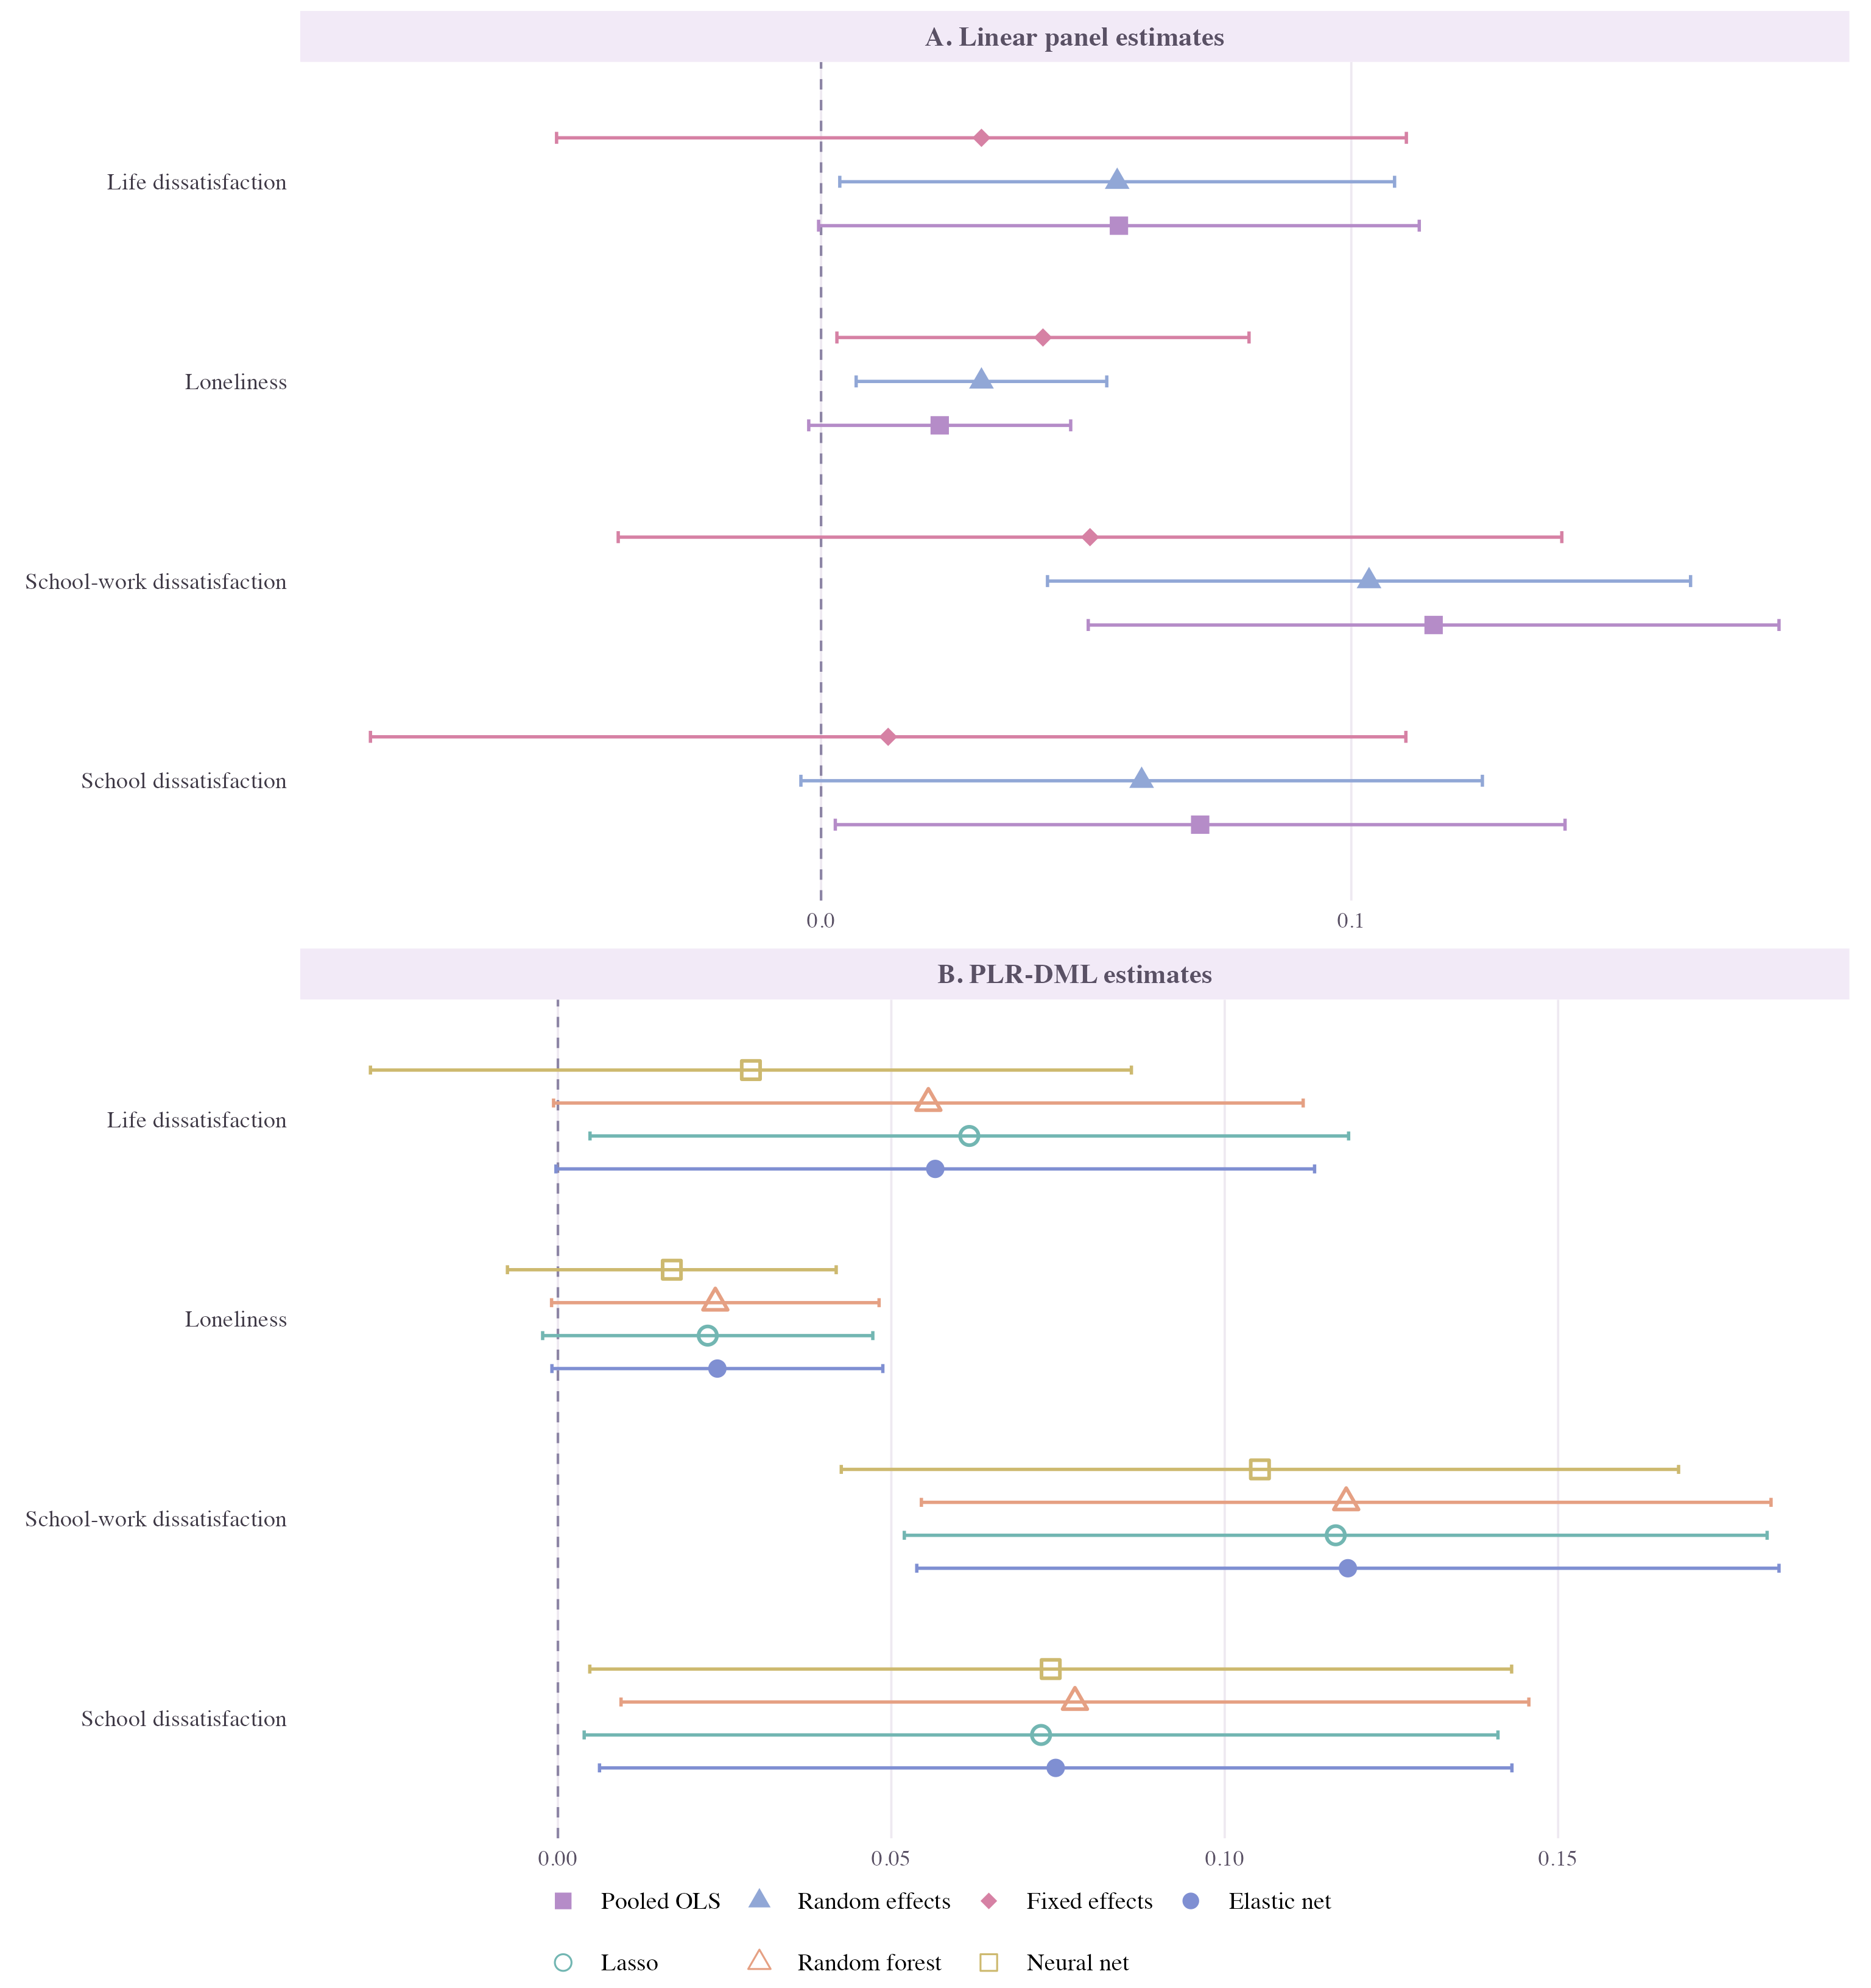
\includegraphics[width=1.05\textwidth,height=0.76\textheight,keepaspectratio]{figures/results_chapter_summary.png}}
\caption{Overview of the principal coefficient estimates. Panels A and B report the linear panel and ordered-treatment PLR-DML weekday estimates for all four outcomes. Lines are 95\% confidence intervals; the outcome-specific samples contain between 4,298 and 4,329 person-wave observations.}
\label{fig:results_chapter_summary}
\end{figure}

\begin{figure}[p]
\centering
\makebox[\textwidth][c]{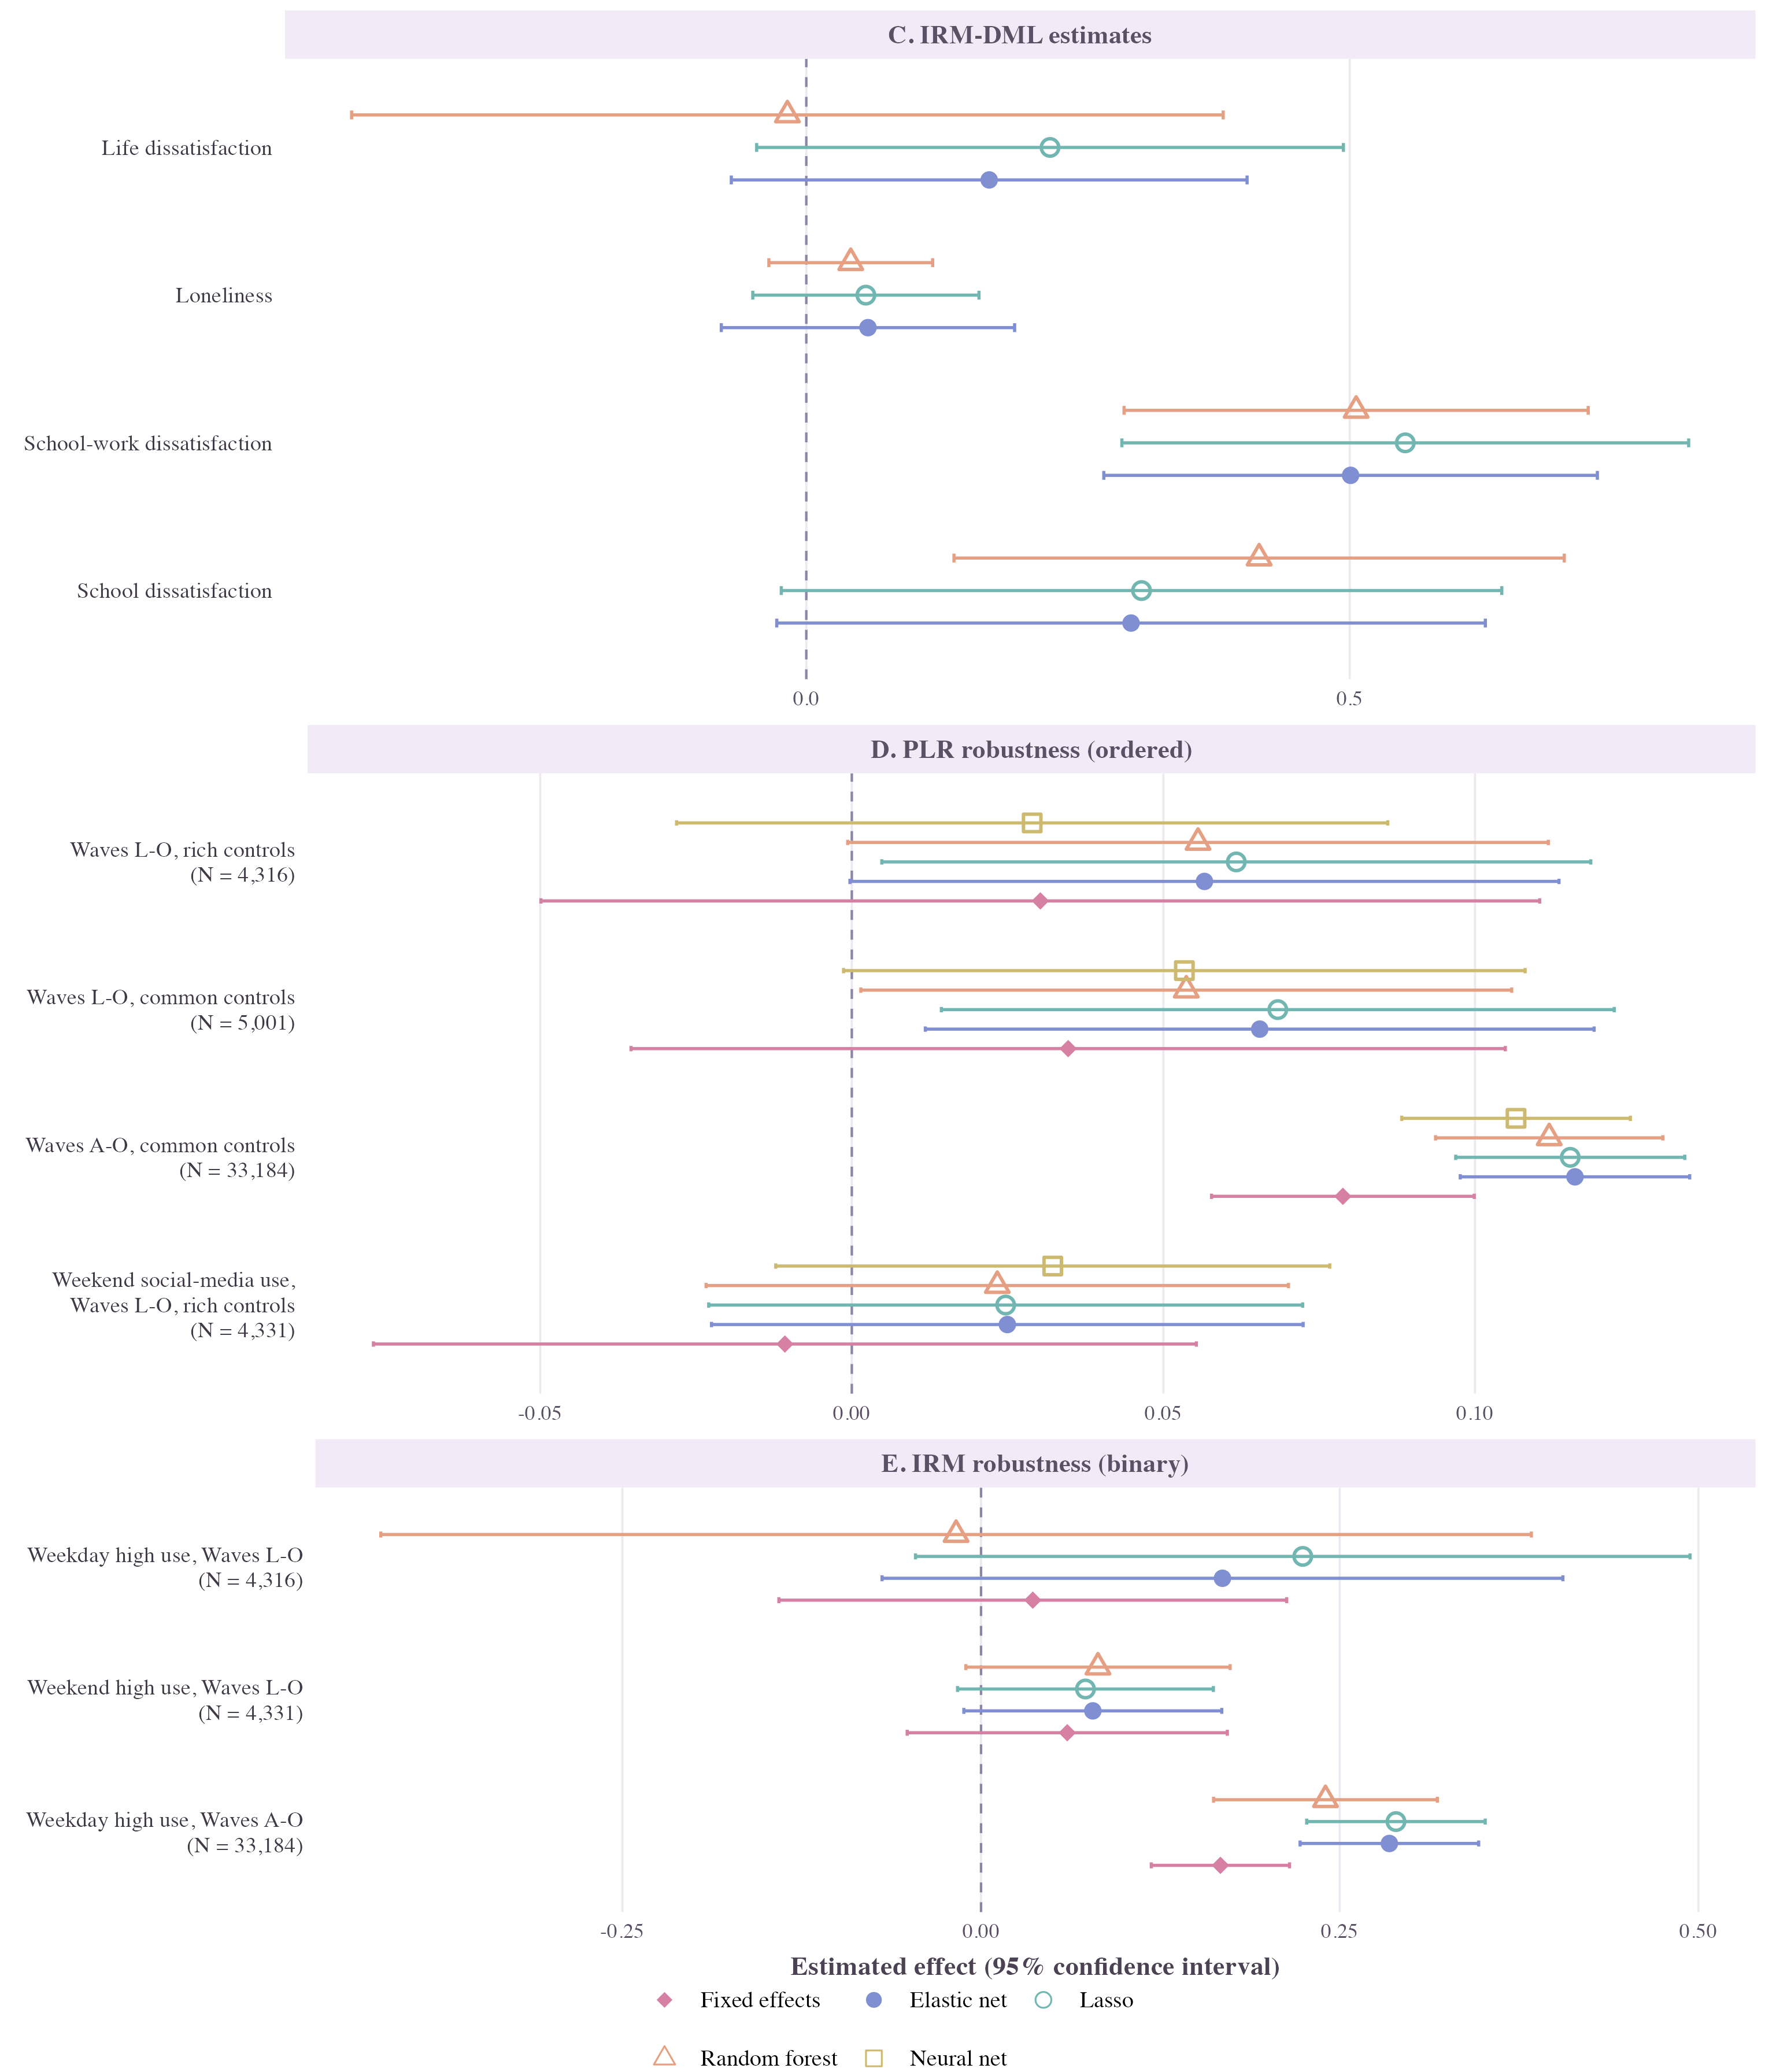
\includegraphics[width=1.05\textwidth,height=0.76\textheight,keepaspectratio]{figures/results_chapter_summary_robustness.png}}
\caption{Overview of the DML and robustness estimates. Panel C reports binary-treatment IRM-DML weekday estimates for all outcomes. For life dissatisfaction, Panel D reports ordered-treatment FE and PLR-DML robustness specifications, while Panel E reports binary-treatment FE and IRM-DML comparisons for weekday use in Waves \texttt{l}--\texttt{o}, weekend use in Waves \texttt{l}--\texttt{o}, and weekday use in Waves \texttt{a}--\texttt{o}. These results come from Tables \ref{tab:fe_dml_comparison}, \ref{tab:robustness_weekend}, and \ref{tab:robustness_extended_waves}.}
\label{fig:results_chapter_summary_robustness}
\end{figure}

\tocchapter{Conclusion and Discussion}{Conclusion and discussion}
\label{chap:conc}

This thesis asked whether heavier weekday social-media use is associated with worse adolescent mental wellbeing after flexible adjustment for confounding, and whether Double Machine Learning changes the conclusion from standard panel models. Weekday use is positively associated with all four adverse outcomes in the pooled models, but the associations shrink after adding the rich controls and become smaller again when fixed effects use only within-adolescent changes. Because the recent-wave panel is short and unbalanced, these fixed-effects estimates should be read as within-adolescent estimates based on the repeatedly observed part of the sample; the unbalanced structure does not invalidate fixed-effects estimation, but it limits precision and affects comparison with pooled estimates. This attenuation is consistent with persistent differences between adolescents explaining an important part of the raw gradient. The remaining magnitude is modest: a representative PLR coefficient of \(0.056\) for life dissatisfaction equals about \(0.044\) outcome standard deviations per treatment category, or \(0.175\) standard deviations across the full four-category contrast if the linear slope is extrapolated. This describes scale, not the causal effect of moving an adolescent between categories.

DML changes the modelling flexibility more than the central empirical message. The ordered-treatment PLR-DML estimates remain positive across learners, but none differs statistically from the preferred fixed-effects estimate for any outcome. The binary IRM results are more learner-sensitive and differ from fixed effects for some school outcomes, while the all-wave estimates are larger than the recent-wave baseline. The comparison therefore does not uncover one hidden effect missed by conventional regression. It shows instead that results depend on identifying variation, treatment definition, survey period, overlap, and learner choice. Machine learning can relax functional-form restrictions, but it cannot resolve unobserved confounding or make different estimands interchangeable.

In practice, the findings do not justify a universal screen-time threshold or the claim that social-media use is uniformly harmful. The weaker weekend result and fixed-effects attenuation argue against treating hours alone as a complete measure of risk. This is consistent with the review by \citet{valkenburg2022umbrella} and the National Academies' conclusion that social media can produce harms or benefits depending on the user, design feature, and form of engagement \citep{nasem2024socialmedia}. Families, schools, and youth professionals should therefore pay attention to whether use displaces sleep, schoolwork, offline relationships, or other valued activities, and to experiences such as loss of control, harassment, and harmful content. WHO evidence similarly distinguishes heavy non-problematic use from problematic use and emphasizes digital literacy rather than treating all intensive engagement as harmful \citep{whoeurope2024screens}. For policy, this favours targeted and evaluable measures, including age-appropriate design, accessible support systems, digital-media literacy, and transparency about recommendation systems, over restrictions based only on minutes of use.

The results also contribute to theory. Modest average associations alongside substantial between-person and period variation are consistent with the Differential Susceptibility to Media Effects Model, in which developmental, dispositional, and social characteristics shape responses to media \citep{valkenburgpeter2013dsmm}. An average coefficient can therefore coexist with benefits for some adolescents, negligible effects for many, and harm for others. Future work should focus more directly on mechanisms and heterogeneous effects. The developmental windows identified by \citet{orben2022windows} and person-specific effects documented by \citet{beyens2020effect} motivate analyses by age and sex, provided that group differences are tested directly and multiple comparisons are handled transparently.

Two limitations define the most important research directions. First, use is self-reported in broad categories. \citet{parry2021discrepancies} show that self-reported digital-media use corresponds only moderately with logged use. Future longitudinal studies should combine surveys with consented device logs or platform data distinguishing platform, content, active and passive engagement, and time of day. This would reduce measurement error and permit direct tests of sleep displacement, social comparison, cyberbullying, and peer support. Second, the sensitivity analysis shows that omitted confounding of plausible strength could move the PLR estimates to zero. Flexible adjustment should therefore be combined with stronger identification from randomized digital-wellbeing interventions, platform or school-policy changes, credible natural experiments, or richer longitudinal designs. Methodologically, future work could integrate respondent fixed effects, clustered cross-fitting, heterogeneous treatment effects, and measurement-error corrections within DML. Access to real-world platform data and stronger causal designs are likewise central recommendations of the National Academies \citep{nasem2024socialmedia}.

Overall, the thesis finds a consistent positive pooled association between weekday social-media use and worse adolescent wellbeing, but limited evidence of a precisely estimated within-adolescent effect and no fully identified universal causal effect. Its broader contribution is to demonstrate why conclusions should not rest on one estimator: panel models reveal the importance of stable individual heterogeneity, DML tests flexible observed-confounder adjustment, and overlap and sensitivity diagnostics show where uncertainty remains. The most credible implication is targeted protection combined with better measurement and transparent policy evaluation, rather than either complacency or a blanket prohibition.

\appendix

\bodychapter{Appendix}

Additional tables, coding details, and supplementary robustness results are reported in the appendix.

\tocsection{Panel Specification Formulas}{Panel specification formulas}
\label{app:spec_tests}
This section collects the main panel-specification formulas used to motivate Section \ref{sec:choice_model_spec}. The presentation follows the pooled time-series exposition and appendix formulas in \citet{ward1993pooled}, with notation adapted to the current thesis.

For the comparison between a fixed-effects model and a pooled classical linear regression model, Ward and Leigh express the global F test for the increase in model fit as
\begin{equation*}
F_{(D,\;NT-K-D)}=
\frac{\left(R^2_{FE}-R^2_{CLR}\right)/D}
{\left(1-R^2_{FE}\right)/(NT-K-D)},
\end{equation*}
where \(N\) is the number of individuals, \(T\) is the number of time periods, \(K\) is the number of regressors in the pooled classical linear regression model, and \(D\) is the number of dummy variables added in the fixed-effects model. The null hypothesis is that the coefficients on all \(D\) dummy variables are jointly zero.

In that setup, the corresponding disturbance assumptions are
\begin{align*}
\mathbb{E}[\varepsilon_{it}] &= 0, \\
\mathrm{Var}(\varepsilon_{it}) &= \sigma^2, \\
\mathrm{Cov}(\varepsilon_{it}, \varepsilon_{js}) &= 0
\qquad \text{for } i \neq j \text{ or } t \neq s.
\end{align*}

For the comparison between a random-effects model and a pooled classical linear regression model, the Breusch--Pagan Lagrange Multiplier test for error components can be written as
\begin{equation*}
LM=
\frac{NT}{2(T-1)}
\left[
\left(
\frac{\sum_i \left(\sum_t \varepsilon_{it}\right)^2}
{\sum_i \sum_t \varepsilon_{it}^2}
\right)
-1
\right]^2,
\end{equation*}
which is asymptotically chi-squared with one degree of freedom under the null hypothesis that the respondent-level variance component is zero. In the current empirical implementation, the thesis uses the Breusch--Pagan LM error-components test available in \texttt{plm}, with the unbalanced-panel extension.

For the comparison between random effects and fixed effects, the Hausman specification test can be written as
\begin{equation*}
H=
\left(\hat{\beta}_{RE}-\hat{\beta}_{FE}\right)'
\left[
\mathrm{Var}\!\left(\hat{\beta}_{FE}\right)
-\mathrm{Var}\!\left(\hat{\beta}_{RE}\right)
\right]^{-1}
\left(\hat{\beta}_{RE}-\hat{\beta}_{FE}\right),
\end{equation*}
which is asymptotically chi-squared under the null that the random-effects estimator is consistent.

\tocsection{Orthogonalization and Moment Conditions}{Orthogonalization and moment conditions}
\label{app:dml_derivations}

This section provides the detailed derivations behind the general results in Section \ref{sec:dml_background}.\footnote{The broad ordering of the discussion from prediction-focused adjustment to orthogonal estimation is informed by \citet{helal2026returns}. The detailed moment derivations and asymptotic arguments follow the original econometric sources, especially \citet{robinson1988rootn} and \citet{chernozhukov2018dml}, and are adapted here to the panel notation of this thesis.} Let \(n\) denote the number of observed person-wave records and let \(\mathbb{E}_n\) denote their sample average.\footnote{The derivations suppress cluster notation for readability. In the application, repeated records are clustered within respondents, folds are assigned at the respondent level, and the LLN and CLT arguments are understood in their independent-cluster form. Because each respondent contributes at most four waves, the number of person-wave observations and the number of respondent clusters grow at the same rate.} The partially linear model is
\begin{align*}
Y_{it} &= \beta_0D_{it}+g_0(X_{it})+U_{it},
& \mathbb{E}[U_{it}\mid D_{it},X_{it}]&=0, \\
D_{it} &= m_0(X_{it})+V_{it},
& \mathbb{E}[V_{it}\mid X_{it}]&=0,
\end{align*}
and
\begin{equation*}
\ell_0(X_{it})
:=
\mathbb{E}[Y_{it}\mid X_{it}]
=
\beta_0m_0(X_{it})+g_0(X_{it}).
\end{equation*}

\subsection[Moment Conditions]{Moment conditions}

The moment conditions below follow directly from the structural and treatment equations. Their derivation repeatedly uses the law of iterated expectations (LIE),
\begin{equation*}
\mathbb{E}[A]
=
\mathbb{E}\!\left[\mathbb{E}[A\mid B]\right].
\end{equation*}

Three population moments clarify why the thesis uses the orthogonal partialling-out score. The first follows directly from the structural equation:
\begin{align*}
\mathbb{E}\!\left[
\bigl(Y_{it}-D_{it}\beta_0-g_0(X_{it})\bigr)D_{it}
\right]
&=
\mathbb{E}[U_{it}D_{it}] \\
&\overset{\mathrm{LIE}}{=}
\mathbb{E}\!\left[
D_{it}\mathbb{E}[U_{it}\mid D_{it},X_{it}]
\right]
=0.
\end{align*}
This is the regression-adjustment moment.

The second moment residualizes the treatment:
\begin{align*}
\mathbb{E}\!\left[
\bigl(Y_{it}-D_{it}\beta_0\bigr)
\bigl(D_{it}-m_0(X_{it})\bigr)
\right]
&=
\mathbb{E}\!\left[
\bigl(g_0(X_{it})+U_{it}\bigr)V_{it}
\right] \\
&=
\mathbb{E}[g_0(X_{it})V_{it}]
+\mathbb{E}[U_{it}V_{it}] \\
&\overset{\mathrm{LIE}}{=}
\mathbb{E}\!\left[
g_0(X_{it})\mathbb{E}[V_{it}\mid X_{it}]
\right] \\
&\quad+
\mathbb{E}\!\left[
V_{it}\mathbb{E}[U_{it}\mid D_{it},X_{it}]
\right]
=0.
\end{align*}
This is the treatment-adjustment moment.

The third residualizes both sides. Since
\begin{align*}
Y_{it}-\ell_0(X_{it})
&=
\beta_0D_{it}+g_0(X_{it})+U_{it}
-\beta_0m_0(X_{it})-g_0(X_{it}) \\
&=
\beta_0\bigl(D_{it}-m_0(X_{it})\bigr)+U_{it},
\end{align*}
it follows that
\begin{align*}
&\mathbb{E}\!\left[
\left\{
Y_{it}-\ell_0(X_{it})
-\beta_0\bigl(D_{it}-m_0(X_{it})\bigr)
\right\}
\bigl(D_{it}-m_0(X_{it})\bigr)
\right] \\
&\qquad =
\mathbb{E}[U_{it}V_{it}] \\
&\qquad \overset{\mathrm{LIE}}{=}
\mathbb{E}\!\left[
V_{it}\mathbb{E}[U_{it}\mid D_{it},X_{it}]
\right]
=0.
\end{align*}
The first two moments show where a one-sided plug-in error can enter. The third is the orthogonal moment used by DML \citep{robinson1988rootn,chernozhukov2018dml}.

\subsection[Why Naive Prediction-Focused ML Is Biased]{Why naive prediction-focused ML is biased}

Suppose that a regularized learner estimates \(g_0(X_{it})\) and the estimate is inserted directly into the regression-adjustment moment:
\begin{equation*}
\frac{1}{n}\sum_{i,t}
D_{it}\bigl(Y_{it}-D_{it}\beta-\widehat{g}(X_{it})\bigr)
=0.
\end{equation*}
Solving for \(\beta\) gives
\begin{equation*}
\widehat{\beta}^{\,RA}
=
\left(
\frac{1}{n}\sum_{i,t}D_{it}^{\,2}
\right)^{-1}
\frac{1}{n}\sum_{i,t}
D_{it}\bigl(Y_{it}-\widehat{g}(X_{it})\bigr).
\end{equation*}
Subtracting \(\beta_0\), substituting the structural equation, and multiplying by \(\sqrt{n}\) yields
\begin{equation*}
\sqrt{n}\bigl(\widehat{\beta}^{\,RA}-\beta_0\bigr)
=
A_n^{RA}+B_n^{RA},
\end{equation*}
where
\begin{align*}
A_n^{RA}
&=
\left(
\frac{1}{n}\sum_{i,t}D_{it}^{\,2}
\right)^{-1}
\frac{1}{\sqrt{n}}\sum_{i,t}D_{it}U_{it}, \\
B_n^{RA}
&=
\left(
\frac{1}{n}\sum_{i,t}D_{it}^{\,2}
\right)^{-1}
\frac{1}{\sqrt{n}}\sum_{i,t}
D_{it}\bigl(g_0(X_{it})-\widehat{g}(X_{it})\bigr).
\end{align*}

The first term is the usual stochastic component. Under finite second moments, the law of large numbers gives
\begin{equation*}
\frac{1}{n}\sum_{i,t}D_{it}^{\,2}
\overset{p}{\longrightarrow}
\mathbb{E}[D_{it}^{\,2}]>0,
\end{equation*}
while a central limit theorem gives
\begin{equation*}
\frac{1}{\sqrt{n}}\sum_{i,t}D_{it}U_{it}
\rightsquigarrow
N(0,\Omega_{RA}).
\end{equation*}
Here \(\Omega_{RA}\) denotes the variance of the respondent-level cluster contribution and therefore allows observations from the same adolescent to be correlated across waves. Slutsky's theorem implies that \(A_n^{RA}\) is asymptotically normal.

The problem is \(B_n^{RA}\). Using \(D_{it}=m_0(X_{it})+V_{it}\), its leading component can be written heuristically as
\begin{align*}
B_n^{RA}
&=
\left(
\frac{1}{n}\sum_{i,t}D_{it}^{\,2}
\right)^{-1}
\frac{1}{\sqrt{n}}\sum_{i,t}
\bigl(m_0(X_{it})+V_{it}\bigr)
\bigl(g_0(X_{it})-\widehat{g}(X_{it})\bigr) \\
&\approx
\bigl(\mathbb{E}[D_{it}^{\,2}]\bigr)^{-1}
\frac{1}{\sqrt{n}}\sum_{i,t}
m_0(X_{it})
\bigl(g_0(X_{it})-\widehat{g}(X_{it})\bigr).
\end{align*}
If the nuisance error satisfies
\begin{equation*}
g_0(X_{it})-\widehat{g}(X_{it})
=
O_p(n^{-\varphi}),
\qquad
0<\varphi<\frac{1}{2},
\end{equation*}
then the scaled bias behaves like
\begin{equation*}
\sqrt{n}\,n^{-\varphi}
=
n^{1/2-\varphi},
\end{equation*}
which does not converge to zero. The naive regression-adjustment estimator is therefore not generally root-\(n\) consistent.

The same issue appears for the treatment-adjustment moment. Its empirical estimator is
\begin{equation*}
\widehat{\beta}^{\,PA}
=
\left[
\frac{1}{n}\sum_{i,t}
D_{it}\bigl(D_{it}-\widehat{m}(X_{it})\bigr)
\right]^{-1}
\frac{1}{n}\sum_{i,t}
Y_{it}\bigl(D_{it}-\widehat{m}(X_{it})\bigr).
\end{equation*}
After subtracting \(\beta_0\),
\begin{equation*}
\sqrt{n}\bigl(\widehat{\beta}^{\,PA}-\beta_0\bigr)
=
A_n^{PA}+B_n^{PA},
\end{equation*}
where the leading bias term contains
\begin{equation*}
\frac{1}{\sqrt{n}}\sum_{i,t}
\bigl(g_0(X_{it})+U_{it}\bigr)
\bigl(m_0(X_{it})-\widehat{m}(X_{it})\bigr).
\end{equation*}
Thus, if \(m_0-\widehat{m}=O_p(n^{-\varphi})\) with \(\varphi<1/2\), this estimator has the same first-order problem \citep{chernozhukov2018dml}.

\subsection[Orthogonalization and the Second-Order Bias]{Orthogonalization and the second-order bias}

The orthogonal solution residualizes both the outcome and treatment:
\begin{equation*}
\widehat{W}_{it}
=
Y_{it}-\widehat{\ell}(X_{it}),
\qquad
\widehat{V}_{it}
=
D_{it}-\widehat{m}(X_{it}).
\end{equation*}
The empirical orthogonal moment is
\begin{equation*}
\frac{1}{n}\sum_{i,t}
\left[
Y_{it}-\widehat{\ell}(X_{it})
-\beta\bigl(D_{it}-\widehat{m}(X_{it})\bigr)
\right]
\bigl(D_{it}-\widehat{m}(X_{it})\bigr)
=0,
\end{equation*}
which gives
\begin{equation*}
\check{\beta}
=
\left(
\frac{1}{n}\sum_{i,t}\widehat{V}_{it}^{\,2}
\right)^{-1}
\frac{1}{n}\sum_{i,t}\widehat{V}_{it}\widehat{W}_{it}.
\end{equation*}

Subtracting \(\beta_0\) gives
\begin{equation*}
\check{\beta}-\beta_0
=
\left(
\frac{1}{n}\sum_{i,t}\widehat{V}_{it}^{\,2}
\right)^{-1}
\frac{1}{n}\sum_{i,t}
\widehat{V}_{it}
\left[
Y_{it}-\widehat{\ell}(X_{it})
-\beta_0\bigl(D_{it}-\widehat{m}(X_{it})\bigr)
\right].
\end{equation*}

Define
\begin{equation*}
\Delta_{\ell,it}
:=
\ell_0(X_{it})-\widehat{\ell}(X_{it}),
\qquad
\Delta_{m,it}
:=
m_0(X_{it})-\widehat{m}(X_{it}).
\end{equation*}
Then
\begin{equation*}
\widehat{V}_{it}
=
V_{it}+\Delta_{m,it},
\end{equation*}
and
\begin{equation*}
Y_{it}-\widehat{\ell}(X_{it})
-\beta_0\bigl(D_{it}-\widehat{m}(X_{it})\bigr)
=
U_{it}+\Delta_{\ell,it}-\beta_0\Delta_{m,it}.
\end{equation*}
Multiplying these expressions gives
\begin{align*}
&\widehat{V}_{it}
\left[
Y_{it}-\widehat{\ell}(X_{it})
-\beta_0\bigl(D_{it}-\widehat{m}(X_{it})\bigr)
\right] \\
&\qquad =
V_{it}U_{it}
+\Delta_{m,it}\Delta_{\ell,it} \\
&\qquad\quad+
\left[
V_{it}\Delta_{\ell,it}
-\beta_0V_{it}\Delta_{m,it}
+\Delta_{m,it}U_{it}
-\beta_0\Delta_{m,it}^{\,2}
\right].
\end{align*}
The resulting asymptotic expansion can be organized as
\begin{equation*}
\sqrt{n}\bigl(\check{\beta}-\beta_0\bigr)
=
A_n^{PO}+B_n^{PO}+R_n,
\end{equation*}
where
\begin{align*}
A_n^{PO}
&=
\left(
\frac{1}{n}\sum_{i,t}V_{it}^{\,2}
\right)^{-1}
\frac{1}{\sqrt{n}}\sum_{i,t}V_{it}U_{it}, \\
B_n^{PO}
&=
\left(
\frac{1}{n}\sum_{i,t}V_{it}^{\,2}
\right)^{-1}
\frac{1}{\sqrt{n}}\sum_{i,t}
\Delta_{m,it}\Delta_{\ell,it},
\end{align*}
and \(R_n\) collects the remaining linear nuisance terms, the squared treatment-nuisance error, and denominator-replacement terms.

For the leading stochastic term, the law of large numbers gives
\begin{equation*}
\frac{1}{n}\sum_{i,t}V_{it}^{\,2}
\overset{p}{\longrightarrow}
\mathbb{E}[V_{it}^{\,2}]>0,
\end{equation*}
and a central limit theorem gives
\begin{equation*}
\frac{1}{\sqrt{n}}\sum_{i,t}V_{it}U_{it}
\rightsquigarrow
N\!\left(
0,
\mathbb{E}\!\left[V_{it}^{\,2}U_{it}^{\,2}\right]
\right).
\end{equation*}
Hence \(A_n^{PO}\) is asymptotically normal by Slutsky's theorem. As noted at the beginning of this section, the empirical implementation uses the respondent-cluster analogue of this variance to allow observations from the same adolescent to be correlated across waves.

Unlike the naive estimators, the leading nuisance component now depends on a product of estimation errors. If
\begin{equation*}
\widehat{m}-m_0
=
O_p(n^{-\varphi_m}),
\qquad
\widehat{\ell}-\ell_0
=
O_p(n^{-\varphi_{\ell}}),
\end{equation*}
then
\begin{equation*}
B_n^{PO}
\asymp
\sqrt{n}\,
n^{-(\varphi_m+\varphi_{\ell})}.
\end{equation*}
If \(\varphi_m+\varphi_{\ell}>1/2\), the leading bias is \(o_p(1)\). A sufficient symmetric case is that both nuisance estimators converge slightly faster than \(n^{-1/4}\). Under the additional control of \(R_n\), this gives
\begin{equation*}
\sqrt{n}\bigl(\check{\beta}-\beta_0\bigr)
\rightsquigarrow
N(0,\Sigma)
\end{equation*}
for an appropriate asymptotic variance \(\Sigma\) \citep{chernozhukov2018dml}.

The third moment condition now suggests defining the score by replacing the unknown nuisance functions with generic candidates. Let
\begin{equation*}
W_{it}=(Y_{it},D_{it},X_{it}),
\qquad
\eta_0=(\ell_0,m_0),
\qquad
\eta=(\ell,m).
\end{equation*}
The partialling-out score used in the thesis is
\begin{align*}
\psi(W_{it};\beta,\eta)
&=
\left[
Y_{it}-\ell(X_{it})
-\beta\bigl(D_{it}-m(X_{it})\bigr)
\right]
\left[
D_{it}-m(X_{it})
\right] \\
&=
-\bigl(D_{it}-m(X_{it})\bigr)^2\beta
+\bigl(Y_{it}-\ell(X_{it})\bigr)
\bigl(D_{it}-m(X_{it})\bigr) \\
&=
\psi_a(W_{it};\eta)\beta+\psi_b(W_{it};\eta),
\end{align*}
with
\begin{align*}
\psi_a(W_{it};\eta)
&=
-\bigl(D_{it}-m(X_{it})\bigr)^2, \\
\psi_b(W_{it};\eta)
&=
\bigl(Y_{it}-\ell(X_{it})\bigr)
\bigl(D_{it}-m(X_{it})\bigr).
\end{align*}
Because the score is linear in the target parameter, its empirical moment condition
\begin{equation*}
\mathbb{E}_n\!\left[
\psi(W_{it};\widetilde{\beta},\widehat{\eta})
\right]
=0
\end{equation*}
can be solved as
\begin{equation*}
\widetilde{\beta}
=
-\frac{
\mathbb{E}_n[\psi_b(W_{it};\widehat{\eta})]
}{
\mathbb{E}_n[\psi_a(W_{it};\widehat{\eta})]
}.
\end{equation*}
Substituting the expressions for \(\psi_a\) and \(\psi_b\) shows that \(\widetilde{\beta}\) is exactly the residual-on-residual estimator \(\check{\beta}\) derived above.

At the population nuisance functions, the third moment condition becomes the identifying score condition
\begin{equation*}
\mathbb{E}\!\left[
\psi(W_{it};\beta_0,\eta_0)
\right]
=0.
\end{equation*}
The corresponding Jacobian with respect to \(\beta\) is
\begin{align*}
J_0
&=
\mathbb{E}\!\left[
\psi_a(W_{it};\eta_0)
\right] \\
&=
-\mathbb{E}\!\left[
\bigl(D_{it}-m_0(X_{it})\bigr)^2
\right] \\
&=
-\mathbb{E}[V_{it}^{\,2}]
\neq 0.
\end{align*}
Thus, identification of \(\beta_0\) requires non-degenerate residual treatment variation after conditioning on \(X_{it}\). This score representation also provides the starting point for verifying Neyman orthogonality \citep{robinson1988rootn,chernozhukov2018dml}.

\subsection[Neyman Orthogonality]{Neyman orthogonality}

To verify that the partialling-out score is Neyman orthogonal, let
\begin{equation*}
\eta_r
=
\bigl(\ell_0+rh_{\ell},m_0+rh_m\bigr),
\qquad
r\in[0,1).
\end{equation*}
Using
\begin{equation*}
Y_{it}-\ell_0(X_{it})
-\beta_0\bigl(D_{it}-m_0(X_{it})\bigr)
=
U_{it},
\qquad
D_{it}-m_0(X_{it})
=
V_{it},
\end{equation*}
the perturbed partialling-out score becomes
\begin{equation*}
\psi(W_{it};\beta_0,\eta_r)
=
\left[
U_{it}+r\bigl(\beta_0h_m(X_{it})-h_{\ell}(X_{it})\bigr)
\right]
\left[
V_{it}-rh_m(X_{it})
\right].
\end{equation*}
Differentiating its expectation at \(r=0\) gives
\begin{align*}
&\left.
\partial_r
\mathbb{E}\!\left[
\psi(W_{it};\beta_0,\eta_r)
\right]
\right|_{r=0} \\
&\qquad =
\mathbb{E}\!\left[
\bigl(\beta_0h_m(X_{it})-h_{\ell}(X_{it})\bigr)V_{it}
\right]
-\mathbb{E}[U_{it}h_m(X_{it})] \\
&\qquad \overset{\mathrm{LIE}}{=}
\mathbb{E}\!\left[
\bigl(\beta_0h_m(X_{it})-h_{\ell}(X_{it})\bigr)
\mathbb{E}[V_{it}\mid X_{it}]
\right] \\
&\qquad\quad-
\mathbb{E}\!\left[
h_m(X_{it})
\mathbb{E}[U_{it}\mid D_{it},X_{it}]
\right]
=0.
\end{align*}
The score is therefore locally insensitive to first-order perturbations of the nuisance functions.

\FloatBarrier
\tocsection{Additional Linear Model Tables}{Additional linear model tables}

\begin{table}[!htbp]
\centering
\caption{Linear model estimates for loneliness}
\label{tab:linear_models_loneliness}
\scriptsize
\setlength{\tabcolsep}{3.2pt}
\renewcommand{\arraystretch}{0.9}
\begin{tabular}{p{0.34\textwidth}cccccc}
\hline
Variable & (1) & (2) & (3) & (4) & (5) & (6) \\
\hline
Weekday social-media use & \shortstack[c]{0.058*** \\[-0.35ex] (0.012)} & \shortstack[c]{0.053*** \\[-0.35ex] (0.012)} & \shortstack[c]{0.022* \\[-0.35ex] (0.013)} & \shortstack[c]{0.042** \\[-0.35ex] (0.020)} & \shortstack[c]{0.042** \\[-0.35ex] (0.020)} & \shortstack[c]{0.030** \\[-0.35ex] (0.012)}
\\
Age &  & \shortstack[c]{0.025*** \\[-0.35ex] (0.006)} & \shortstack[c]{0.013** \\[-0.35ex] (0.006)} & \shortstack[c]{0.045*** \\[-0.35ex] (0.011)} & \shortstack[c]{0.057 \\[-0.35ex] (0.058)} & \shortstack[c]{0.017*** \\[-0.35ex] (0.006)}
\\
Female &  & \shortstack[c]{0.234*** \\[-0.35ex] (0.021)} & \shortstack[c]{0.207*** \\[-0.35ex] (0.021)} &  &  & \shortstack[c]{0.199*** \\[-0.35ex] (0.021)}
\\
Urban area &  & \shortstack[c]{-0.033 \\[-0.35ex] (0.025)} & \shortstack[c]{-0.042 \\[-0.35ex] (0.026)} & \shortstack[c]{0.052 \\[-0.35ex] (0.133)} & \shortstack[c]{0.054 \\[-0.35ex] (0.131)} & \shortstack[c]{-0.038 \\[-0.35ex] (0.025)}
\\
Close friends &  &  & \shortstack[c]{-0.179*** \\[-0.35ex] (0.016)} & \shortstack[c]{-0.164*** \\[-0.35ex] (0.027)} & \shortstack[c]{-0.164*** \\[-0.35ex] (0.027)} & \shortstack[c]{-0.170*** \\[-0.35ex] (0.016)}
\\
Parents/step-parents in household &  &  & \shortstack[c]{-0.002 \\[-0.35ex] (0.023)} & \shortstack[c]{-0.025 \\[-0.35ex] (0.090)} & \shortstack[c]{-0.025 \\[-0.35ex] (0.090)} & \shortstack[c]{0.004 \\[-0.35ex] (0.022)}
\\
Grandparents in household &  &  & \shortstack[c]{-0.015 \\[-0.35ex] (0.036)} & \shortstack[c]{-0.182 \\[-0.35ex] (0.192)} & \shortstack[c]{-0.182 \\[-0.35ex] (0.193)} & \shortstack[c]{-0.004 \\[-0.35ex] (0.039)}
\\
Siblings/step-siblings in household &  &  & \shortstack[c]{-0.032*** \\[-0.35ex] (0.010)} & \shortstack[c]{0.027 \\[-0.35ex] (0.058)} & \shortstack[c]{0.027 \\[-0.35ex] (0.058)} & \shortstack[c]{-0.025** \\[-0.35ex] (0.010)}
\\
Family meals &  &  & \shortstack[c]{-0.054*** \\[-0.35ex] (0.011)} & \shortstack[c]{-0.038* \\[-0.35ex] (0.021)} & \shortstack[c]{-0.038* \\[-0.35ex] (0.021)} & \shortstack[c]{-0.054*** \\[-0.35ex] (0.010)}
\\
Television/video hours &  &  & \shortstack[c]{0.080*** \\[-0.35ex] (0.015)} & \shortstack[c]{-0.001 \\[-0.35ex] (0.021)} & \shortstack[c]{-0.001 \\[-0.35ex] (0.021)} & \shortstack[c]{0.060*** \\[-0.35ex] (0.014)}
\\
Smartphone &  &  & \shortstack[c]{-0.055* \\[-0.35ex] (0.031)} & \shortstack[c]{0.018 \\[-0.35ex] (0.043)} & \shortstack[c]{0.018 \\[-0.35ex] (0.043)} & \shortstack[c]{-0.039 \\[-0.35ex] (0.029)}
\\
Tablet &  &  & \shortstack[c]{-0.011 \\[-0.35ex] (0.019)} & \shortstack[c]{0.002 \\[-0.35ex] (0.032)} & \shortstack[c]{0.002 \\[-0.35ex] (0.032)} & \shortstack[c]{-0.005 \\[-0.35ex] (0.018)}
\\
Gaming console &  &  & \shortstack[c]{0.010 \\[-0.35ex] (0.024)} & \shortstack[c]{0.025 \\[-0.35ex] (0.039)} & \shortstack[c]{0.025 \\[-0.35ex] (0.040)} & \shortstack[c]{0.010 \\[-0.35ex] (0.022)}
\\
Laptop/desktop computer &  &  & \shortstack[c]{0.039 \\[-0.35ex] (0.024)} & \shortstack[c]{0.006 \\[-0.35ex] (0.038)} & \shortstack[c]{0.006 \\[-0.35ex] (0.038)} & \shortstack[c]{0.033 \\[-0.35ex] (0.023)}
\\
\hline
Model & Bivariate & Basic & Rich pooled & FE & FE + wave & RE
\\
$R^2$ & 0.007 & 0.051 & 0.122 & 0.066 & 0.066 & 0.153
\\
N & 4,298 & 4,298 & 4,298 & 4,298 & 4,298 & 4,298
\\
\hline
\end{tabular}
\renewcommand{\arraystretch}{1}
\begin{minipage}{0.97\textwidth}
\footnotesize Notes: All columns use the same common outcome-specific sample and report respondent-clustered standard errors in parentheses below the coefficient. Column (1) is a bivariate pooled OLS model. Column (2) adds age, female, and urban-area controls. Column (3) adds the rich baseline control set in a standard pooled linear regression. Column (4) is a fixed-effects model with rich controls and individual intercepts. Column (5) adds wave fixed effects to the fixed-effects model. Column (6) is a random-effects model with rich controls. Blank cells indicate covariates that are absorbed by individual fixed effects or otherwise not identified in a given specification. The rich-control models also include broad ethnicity and region dummies, which are omitted from display for compactness. The row labeled Close friends refers to the logged control \texttt{log(1 + close\_friends)} used in the regressions. Significance: *** \(p < 0.01\), ** \(p < 0.05\), * \(p < 0.10\).
\end{minipage}
\end{table}


\begin{table}[!htbp]
\centering
\caption{Linear model estimates for school-work dissatisfaction}
\label{tab:linear_models_schoolwork}
\scriptsize
\setlength{\tabcolsep}{3.2pt}
\renewcommand{\arraystretch}{0.9}
\begin{tabular}{p{0.34\textwidth}cccccc}
\hline
Variable & (1) & (2) & (3) & (4) & (5) & (6) \\
\hline
Weekday social-media use & \shortstack[c]{0.204*** \\[-0.35ex] (0.030)} & \shortstack[c]{0.199*** \\[-0.35ex] (0.031)} & \shortstack[c]{0.116*** \\[-0.35ex] (0.033)} & \shortstack[c]{0.052 \\[-0.35ex] (0.045)} & \shortstack[c]{0.051 \\[-0.35ex] (0.045)} & \shortstack[c]{0.103*** \\[-0.35ex] (0.031)}
\\
Age &  & \shortstack[c]{0.022 \\[-0.35ex] (0.015)} & \shortstack[c]{-0.000 \\[-0.35ex] (0.015)} & \shortstack[c]{0.126*** \\[-0.35ex] (0.028)} & \shortstack[c]{-0.193 \\[-0.35ex] (0.136)} & \shortstack[c]{0.029** \\[-0.35ex] (0.014)}
\\
Female &  & \shortstack[c]{0.215*** \\[-0.35ex] (0.051)} & \shortstack[c]{0.239*** \\[-0.35ex] (0.054)} &  &  & \shortstack[c]{0.224*** \\[-0.35ex] (0.053)}
\\
Urban area &  & \shortstack[c]{-0.048 \\[-0.35ex] (0.060)} & \shortstack[c]{-0.061 \\[-0.35ex] (0.063)} & \shortstack[c]{0.175 \\[-0.35ex] (0.382)} & \shortstack[c]{0.117 \\[-0.35ex] (0.390)} & \shortstack[c]{-0.070 \\[-0.35ex] (0.063)}
\\
Close friends &  &  & \shortstack[c]{-0.177*** \\[-0.35ex] (0.040)} & \shortstack[c]{0.028 \\[-0.35ex] (0.064)} & \shortstack[c]{0.025 \\[-0.35ex] (0.064)} & \shortstack[c]{-0.118*** \\[-0.35ex] (0.039)}
\\
Parents/step-parents in household &  &  & \shortstack[c]{-0.186*** \\[-0.35ex] (0.061)} & \shortstack[c]{-0.331** \\[-0.35ex] (0.165)} & \shortstack[c]{-0.324** \\[-0.35ex] (0.163)} & \shortstack[c]{-0.226*** \\[-0.35ex] (0.060)}
\\
Grandparents in household &  &  & \shortstack[c]{-0.021 \\[-0.35ex] (0.098)} & \shortstack[c]{0.499 \\[-0.35ex] (0.507)} & \shortstack[c]{0.495 \\[-0.35ex] (0.507)} & \shortstack[c]{-0.022 \\[-0.35ex] (0.103)}
\\
Siblings/step-siblings in household &  &  & \shortstack[c]{0.011 \\[-0.35ex] (0.026)} & \shortstack[c]{0.102 \\[-0.35ex] (0.152)} & \shortstack[c]{0.109 \\[-0.35ex] (0.159)} & \shortstack[c]{0.021 \\[-0.35ex] (0.026)}
\\
Family meals &  &  & \shortstack[c]{-0.187*** \\[-0.35ex] (0.026)} & \shortstack[c]{-0.098** \\[-0.35ex] (0.049)} & \shortstack[c]{-0.091* \\[-0.35ex] (0.049)} & \shortstack[c]{-0.179*** \\[-0.35ex] (0.025)}
\\
Television/video hours &  &  & \shortstack[c]{0.146*** \\[-0.35ex] (0.041)} & \shortstack[c]{-0.010 \\[-0.35ex] (0.055)} & \shortstack[c]{-0.012 \\[-0.35ex] (0.055)} & \shortstack[c]{0.097*** \\[-0.35ex] (0.036)}
\\
Smartphone &  &  & \shortstack[c]{-0.078 \\[-0.35ex] (0.080)} & \shortstack[c]{0.018 \\[-0.35ex] (0.114)} & \shortstack[c]{0.017 \\[-0.35ex] (0.114)} & \shortstack[c]{-0.055 \\[-0.35ex] (0.076)}
\\
Tablet &  &  & \shortstack[c]{-0.111** \\[-0.35ex] (0.048)} & \shortstack[c]{0.080 \\[-0.35ex] (0.076)} & \shortstack[c]{0.073 \\[-0.35ex] (0.076)} & \shortstack[c]{-0.078* \\[-0.35ex] (0.046)}
\\
Gaming console &  &  & \shortstack[c]{0.128** \\[-0.35ex] (0.058)} & \shortstack[c]{-0.043 \\[-0.35ex] (0.092)} & \shortstack[c]{-0.036 \\[-0.35ex] (0.092)} & \shortstack[c]{0.087 \\[-0.35ex] (0.054)}
\\
Laptop/desktop computer &  &  & \shortstack[c]{-0.070 \\[-0.35ex] (0.060)} & \shortstack[c]{-0.187** \\[-0.35ex] (0.081)} & \shortstack[c]{-0.182** \\[-0.35ex] (0.081)} & \shortstack[c]{-0.099* \\[-0.35ex] (0.055)}
\\
\hline
Model & Bivariate & Basic & Rich pooled & FE & FE + wave & RE
\\
$R^2$ & 0.014 & 0.020 & 0.073 & 0.038 & 0.042 & 0.128
\\
N & 4,329 & 4,329 & 4,329 & 4,329 & 4,329 & 4,329
\\
\hline
\end{tabular}
\renewcommand{\arraystretch}{1}
\begin{minipage}{0.97\textwidth}
\footnotesize Notes: All columns use the same common outcome-specific sample and report respondent-clustered standard errors in parentheses below the coefficient. Column (1) is a bivariate pooled OLS model. Column (2) adds age, female, and urban-area controls. Column (3) adds the rich baseline control set in a standard pooled linear regression. Column (4) is a fixed-effects model with rich controls and individual intercepts. Column (5) adds wave fixed effects to the fixed-effects model. Column (6) is a random-effects model with rich controls. Blank cells indicate covariates that are absorbed by individual fixed effects or otherwise not identified in a given specification. The rich-control models also include broad ethnicity and region dummies, which are omitted from display for compactness. The row labeled Close friends refers to the logged control \texttt{log(1 + close\_friends)} used in the regressions. Significance: *** \(p < 0.01\), ** \(p < 0.05\), * \(p < 0.10\).
\end{minipage}
\end{table}


\begin{table}[!htbp]
\centering
\caption{Linear model estimates for school dissatisfaction}
\label{tab:linear_models_school}
\scriptsize
\setlength{\tabcolsep}{3.2pt}
\renewcommand{\arraystretch}{0.9}
\begin{tabular}{p{0.34\textwidth}cccccc}
\hline
Variable & (1) & (2) & (3) & (4) & (5) & (6) \\
\hline
Weekday social-media use & \shortstack[c]{0.210*** \\[-0.35ex] (0.033)} & \shortstack[c]{0.172*** \\[-0.35ex] (0.033)} & \shortstack[c]{0.071** \\[-0.35ex] (0.035)} & \shortstack[c]{0.014 \\[-0.35ex] (0.049)} & \shortstack[c]{0.013 \\[-0.35ex] (0.050)} & \shortstack[c]{0.060* \\[-0.35ex] (0.033)}
\\
Age &  & \shortstack[c]{0.159*** \\[-0.35ex] (0.015)} & \shortstack[c]{0.134*** \\[-0.35ex] (0.016)} & \shortstack[c]{0.305*** \\[-0.35ex] (0.031)} & \shortstack[c]{0.029 \\[-0.35ex] (0.128)} & \shortstack[c]{0.160*** \\[-0.35ex] (0.015)}
\\
Female &  & \shortstack[c]{0.275*** \\[-0.35ex] (0.056)} & \shortstack[c]{0.243*** \\[-0.35ex] (0.058)} &  &  & \shortstack[c]{0.216*** \\[-0.35ex] (0.057)}
\\
Urban area &  & \shortstack[c]{0.066 \\[-0.35ex] (0.066)} & \shortstack[c]{-0.021 \\[-0.35ex] (0.068)} & \shortstack[c]{0.100 \\[-0.35ex] (0.470)} & \shortstack[c]{0.046 \\[-0.35ex] (0.481)} & \shortstack[c]{0.007 \\[-0.35ex] (0.065)}
\\
Close friends &  &  & \shortstack[c]{-0.352*** \\[-0.35ex] (0.044)} & \shortstack[c]{-0.167** \\[-0.35ex] (0.075)} & \shortstack[c]{-0.170** \\[-0.35ex] (0.075)} & \shortstack[c]{-0.298*** \\[-0.35ex] (0.043)}
\\
Parents/step-parents in household &  &  & \shortstack[c]{-0.075 \\[-0.35ex] (0.062)} & \shortstack[c]{-0.262 \\[-0.35ex] (0.218)} & \shortstack[c]{-0.257 \\[-0.35ex] (0.216)} & \shortstack[c]{-0.109* \\[-0.35ex] (0.061)}
\\
Grandparents in household &  &  & \shortstack[c]{0.035 \\[-0.35ex] (0.117)} & \shortstack[c]{0.352 \\[-0.35ex] (0.550)} & \shortstack[c]{0.359 \\[-0.35ex] (0.552)} & \shortstack[c]{0.020 \\[-0.35ex] (0.116)}
\\
Siblings/step-siblings in household &  &  & \shortstack[c]{0.014 \\[-0.35ex] (0.028)} & \shortstack[c]{-0.012 \\[-0.35ex] (0.134)} & \shortstack[c]{0.006 \\[-0.35ex] (0.138)} & \shortstack[c]{0.018 \\[-0.35ex] (0.027)}
\\
Family meals &  &  & \shortstack[c]{-0.205*** \\[-0.35ex] (0.029)} & \shortstack[c]{-0.047 \\[-0.35ex] (0.053)} & \shortstack[c]{-0.040 \\[-0.35ex] (0.053)} & \shortstack[c]{-0.183*** \\[-0.35ex] (0.027)}
\\
Television/video hours &  &  & \shortstack[c]{0.231*** \\[-0.35ex] (0.040)} & \shortstack[c]{0.002 \\[-0.35ex] (0.055)} & \shortstack[c]{0.003 \\[-0.35ex] (0.055)} & \shortstack[c]{0.164*** \\[-0.35ex] (0.037)}
\\
Smartphone &  &  & \shortstack[c]{-0.101 \\[-0.35ex] (0.082)} & \shortstack[c]{0.060 \\[-0.35ex] (0.113)} & \shortstack[c]{0.062 \\[-0.35ex] (0.113)} & \shortstack[c]{-0.045 \\[-0.35ex] (0.077)}
\\
Tablet &  &  & \shortstack[c]{-0.108** \\[-0.35ex] (0.053)} & \shortstack[c]{0.036 \\[-0.35ex] (0.086)} & \shortstack[c]{0.033 \\[-0.35ex] (0.086)} & \shortstack[c]{-0.076 \\[-0.35ex] (0.050)}
\\
Gaming console &  &  & \shortstack[c]{0.056 \\[-0.35ex] (0.063)} & \shortstack[c]{-0.071 \\[-0.35ex] (0.110)} & \shortstack[c]{-0.073 \\[-0.35ex] (0.110)} & \shortstack[c]{0.025 \\[-0.35ex] (0.060)}
\\
Laptop/desktop computer &  &  & \shortstack[c]{-0.159** \\[-0.35ex] (0.064)} & \shortstack[c]{-0.113 \\[-0.35ex] (0.101)} & \shortstack[c]{-0.104 \\[-0.35ex] (0.100)} & \shortstack[c]{-0.136** \\[-0.35ex] (0.062)}
\\
\hline
Model & Bivariate & Basic & Rich pooled & FE & FE + wave & RE
\\
$R^2$ & 0.012 & 0.047 & 0.115 & 0.091 & 0.094 & 0.132
\\
N & 4,316 & 4,316 & 4,316 & 4,316 & 4,316 & 4,316
\\
\hline
\end{tabular}
\renewcommand{\arraystretch}{1}
\begin{minipage}{0.97\textwidth}
\footnotesize Notes: All columns use the same common outcome-specific sample and report respondent-clustered standard errors in parentheses below the coefficient. Column (1) is a bivariate pooled OLS model. Column (2) adds age, female, and urban-area controls. Column (3) adds the rich baseline control set in a standard pooled linear regression. Column (4) is a fixed-effects model with rich controls and individual intercepts. Column (5) adds wave fixed effects to the fixed-effects model. Column (6) is a random-effects model with rich controls. Blank cells indicate covariates that are absorbed by individual fixed effects or otherwise not identified in a given specification. The rich-control models also include broad ethnicity and region dummies, which are omitted from display for compactness. The row labeled Close friends refers to the logged control \texttt{log(1 + close\_friends)} used in the regressions. Significance: *** \(p < 0.01\), ** \(p < 0.05\), * \(p < 0.10\).
\end{minipage}
\end{table}


\FloatBarrier
\tocsection{Additional Partially Linear Double Machine Learning Tables}{Additional partially linear double machine learning tables}

\input{tables/table_dml_loneliness_methods.tex}

\begin{table}[!htbp]
\centering
\caption{Partially linear double machine learning estimates for school-work dissatisfaction across nuisance learners}
\label{tab:dml_schoolwork_methods}
\begin{tabular}{lcccc}
\hline
Variable & Elastic net & Lasso & Random forest & Neural net
\\
\hline
Weekday social-media use & 0.118*** & 0.117*** & 0.118*** & 0.105***
\\
 & (0.033) & (0.033) & (0.033) & (0.032)
\\
N & 4,329 & 4,329 & 4,329 & 4,329
\\
\hline
\end{tabular}
\begin{minipage}{0.95\textwidth}
\footnotesize Notes: All columns report pooled double machine learning estimates from the partially linear regression specification for the coefficient on weekday social-media use. The same common outcome-specific sample with rich controls is used throughout, and wave fixed effects are included among the controls. Elastic net uses alpha = 0.5, while Lasso uses alpha = 1. Standard errors come from respondent-clustered DoubleML inference with 5-fold cross-fitting. Significance: *** \(p < 0.01\), ** \(p < 0.05\), * \(p < 0.10\).
\end{minipage}
\end{table}


\input{tables/table_dml_school_methods.tex}

\FloatBarrier
\tocsection{Additional Interactive Regression Model Tables}{Additional interactive regression model tables}

\input{tables/table_irm_loneliness_methods.tex}

\input{tables/table_irm_schoolwork_methods.tex}

\begin{table}[!htbp]
\centering
\caption{Interactive regression model double machine learning estimates for school dissatisfaction across nuisance learners}
\label{tab:irm_school_methods}
\begin{tabular}{lccc}
\hline
Variable & Elastic net & Lasso & Random forest
\\
\hline
High social-media use & 0.299* & 0.308* & 0.417***
\\
 & (0.166) & (0.169) & (0.143)
\\
N & 4,316 & 4,316 & 4,316
\\
\hline
\end{tabular}
\begin{minipage}{0.95\textwidth}
\footnotesize Notes: All columns report pooled double machine learning average treatment effect estimates from the interactive regression model for the binary indicator of at least four hours of weekday social-media use. The same common outcome-specific sample with rich controls is used throughout, and wave fixed effects are included among the controls. Elastic net uses alpha = 0.5, while Lasso uses alpha = 1 for both the outcome and propensity nuisances. The interactive-regression comparison is restricted to Elastic net, Lasso, and Random forest because these were the learners that remained numerically stable in the binary-treatment setting. Standard errors come from respondent-clustered DoubleML inference with 5-fold cross-fitting. Significance: *** \(p < 0.01\), ** \(p < 0.05\), * \(p < 0.10\).
\end{minipage}
\end{table}


\FloatBarrier
\tocsection{Additional Fixed-Effects and Double Machine Learning Comparisons}{Additional fixed-effects and double machine learning comparisons}

The following tables extend the paired comparisons in Table \ref{tab:fe_dml_comparison} to the three supplementary outcomes. In each table, Panel A compares the fixed-effects coefficient on the ordered weekday-use measure with the PLR-DML estimates. Panel B uses the binary high-use indicator in both the fixed-effects and IRM-DML specifications. Both estimators are re-estimated in each of 500 respondent-cluster bootstrap replications, so the reported tests incorporate the covariance between the paired estimates.

\begin{table}[!htbp]
\centering
\caption{Paired comparisons of fixed-effects and DML estimates for loneliness}
\label{tab:fe_dml_comparison_loneliness}
\small
\setlength{\tabcolsep}{6pt}
\begin{tabular}{lcccc}
\hline
Statistic & Elastic net & Lasso & Random forest & Neural net
\\
\hline
\multicolumn{5}{l}{\textit{Panel A: Ordered-treatment FE versus PLR-DML}} \\
$t$-statistic & 0.957 & 1.030 & 0.880 & 1.200
\\
$p$-value & 0.338 & 0.303 & 0.379 & 0.230
\\[0.4ex]
\multicolumn{5}{l}{\textit{Panel B: Binary-treatment FE versus IRM-DML}} \\
$t$-statistic & 0.144 & 0.170 & 0.416 & --
\\
$p$-value & 0.886 & 0.865 & 0.678 & --
\\
\hline
\end{tabular}
\begin{minipage}{0.96\textwidth}
\footnotesize Notes: Panel A compares the fixed-effects coefficient on the ordered five-category weekday-use measure with the PLR-DML coefficients in Table~\ref{tab:dml_loneliness_methods}. Panel B compares a separately estimated fixed-effects coefficient on the binary high-use indicator with the IRM-DML average treatment effects in Table~\ref{tab:irm_loneliness_methods}. The neural-net IRM cell is not reported because that learner was not retained in the binary-treatment analysis. For both panels, standard errors of the paired differences use 500 respondent-cluster bootstrap replications, and the two-sided $p$-values use the standard-normal approximation. All comparisons use the same outcome-specific sample with $N=4,298$ person-wave observations.
\end{minipage}
\end{table}


\input{tables/table_fe_dml_comparison_schoolwork_dissatisfaction.tex}

\begin{table}[!htbp]
\centering
\caption{Paired comparisons of fixed-effects and DML estimates for school dissatisfaction}
\label{tab:fe_dml_comparison_school_dissatisfaction}
\small
\setlength{\tabcolsep}{6pt}
\begin{tabular}{lcccc}
\hline
Statistic & Elastic net & Lasso & Random forest & Neural net
\\
\hline
\multicolumn{5}{l}{\textit{Panel A: Ordered-treatment FE versus PLR-DML}} \\
$t$-statistic & -1.256 & -1.215 & -1.175 & -1.133
\\
$p$-value & 0.209 & 0.224 & 0.240 & 0.257
\\[0.4ex]
\multicolumn{5}{l}{\textit{Panel B: Binary-treatment FE versus IRM-DML}} \\
$t$-statistic & -1.355 & -1.362 & -2.339 & --
\\
$p$-value & 0.175 & 0.173 & 0.019 & --
\\
\hline
\end{tabular}
\begin{minipage}{0.96\textwidth}
\footnotesize Notes: Panel A compares the fixed-effects coefficient on the ordered five-category weekday-use measure with the PLR-DML coefficients in Table~\ref{tab:dml_school_methods}. Panel B compares a separately estimated fixed-effects coefficient on the binary high-use indicator with the IRM-DML average treatment effects in Table~\ref{tab:irm_school_methods}. The neural-net IRM cell is not reported because that learner was not retained in the binary-treatment analysis. For both panels, standard errors of the paired differences use 500 respondent-cluster bootstrap replications, and the two-sided $p$-values use the standard-normal approximation. All comparisons use the same outcome-specific sample with $N=4,316$ person-wave observations.
\end{minipage}
\end{table}


\FloatBarrier
\tocsection{Additional Robustness Analyses}{Additional robustness analyses}
\label{sec:additional_robustness}

The following tables and figure provide the diagnostics discussed in Section \ref{sec:robustness_results}. They focus on life dissatisfaction, the main wellbeing outcome, and retain respondent-level fold assignment and clustered inference throughout.

\begin{table}[!htbp]
\centering
\caption{Leave-one-wave-out estimates for life dissatisfaction}
\label{tab:robustness_leave_one_wave_out}
\small
\setlength{\tabcolsep}{4pt}
\begin{tabular}{lcccr}
\hline
Specification & Fixed effects & Elastic net & Random forest & $N$
\\
\hline
Exclude Wave l & 0.007 (0.049) & 0.029 (0.030) & 0.038 (0.030) & 3,705
\\
Exclude Wave m & 0.077 (0.053) & 0.064* (0.035) & 0.060* (0.034) & 2,939
\\
Exclude Wave n & -0.027 (0.057) & 0.052 (0.035) & 0.041 (0.035) & 3,081
\\
Exclude Wave o & 0.046 (0.055) & 0.086*** (0.033) & 0.070** (0.033) & 3,223
\\
\hline
\end{tabular}
\begin{minipage}{0.97\textwidth}
\footnotesize Notes: Each row removes one baseline wave and rebuilds the complete-case sample. Elastic net and random forest represent a penalized linear and a flexible tree-based nuisance specification. Cells report coefficients with respondent-clustered standard errors in parentheses. $^{***}p<0.01$, $^{**}p<0.05$, $^{*}p<0.10$.
\end{minipage}
\end{table}


\begin{table}[!htbp]
\centering
\caption{Repeated cross-fitting robustness for life dissatisfaction}
\label{tab:robustness_repeated_cross_fitting}
\small
\setlength{\tabcolsep}{5pt}
\begin{tabular}{lcccc}
\hline
Learner & Single split & Repeated estimate & Repeated SE & 5th--95th percentile
\\
\hline
Elastic net & 0.057 & 0.059 & 0.029 & [0.054, 0.062]
\\
Lasso & 0.062 & 0.058 & 0.029 & [0.053, 0.062]
\\
Random forest & 0.056 & 0.053 & 0.029 & [0.045, 0.059]
\\
Neural net & 0.029 & 0.042 & 0.028 & [0.017, 0.066]
\\
\hline
\end{tabular}
\begin{minipage}{0.96\textwidth}
\footnotesize Notes: Repeated estimates aggregate 100 independent five-fold respondent-level partitions by their median. The final column describes variation in the treatment estimate across the individual sample splits; it is not a confidence interval.
\end{minipage}
\end{table}


\begin{figure}[!htbp]
\centering
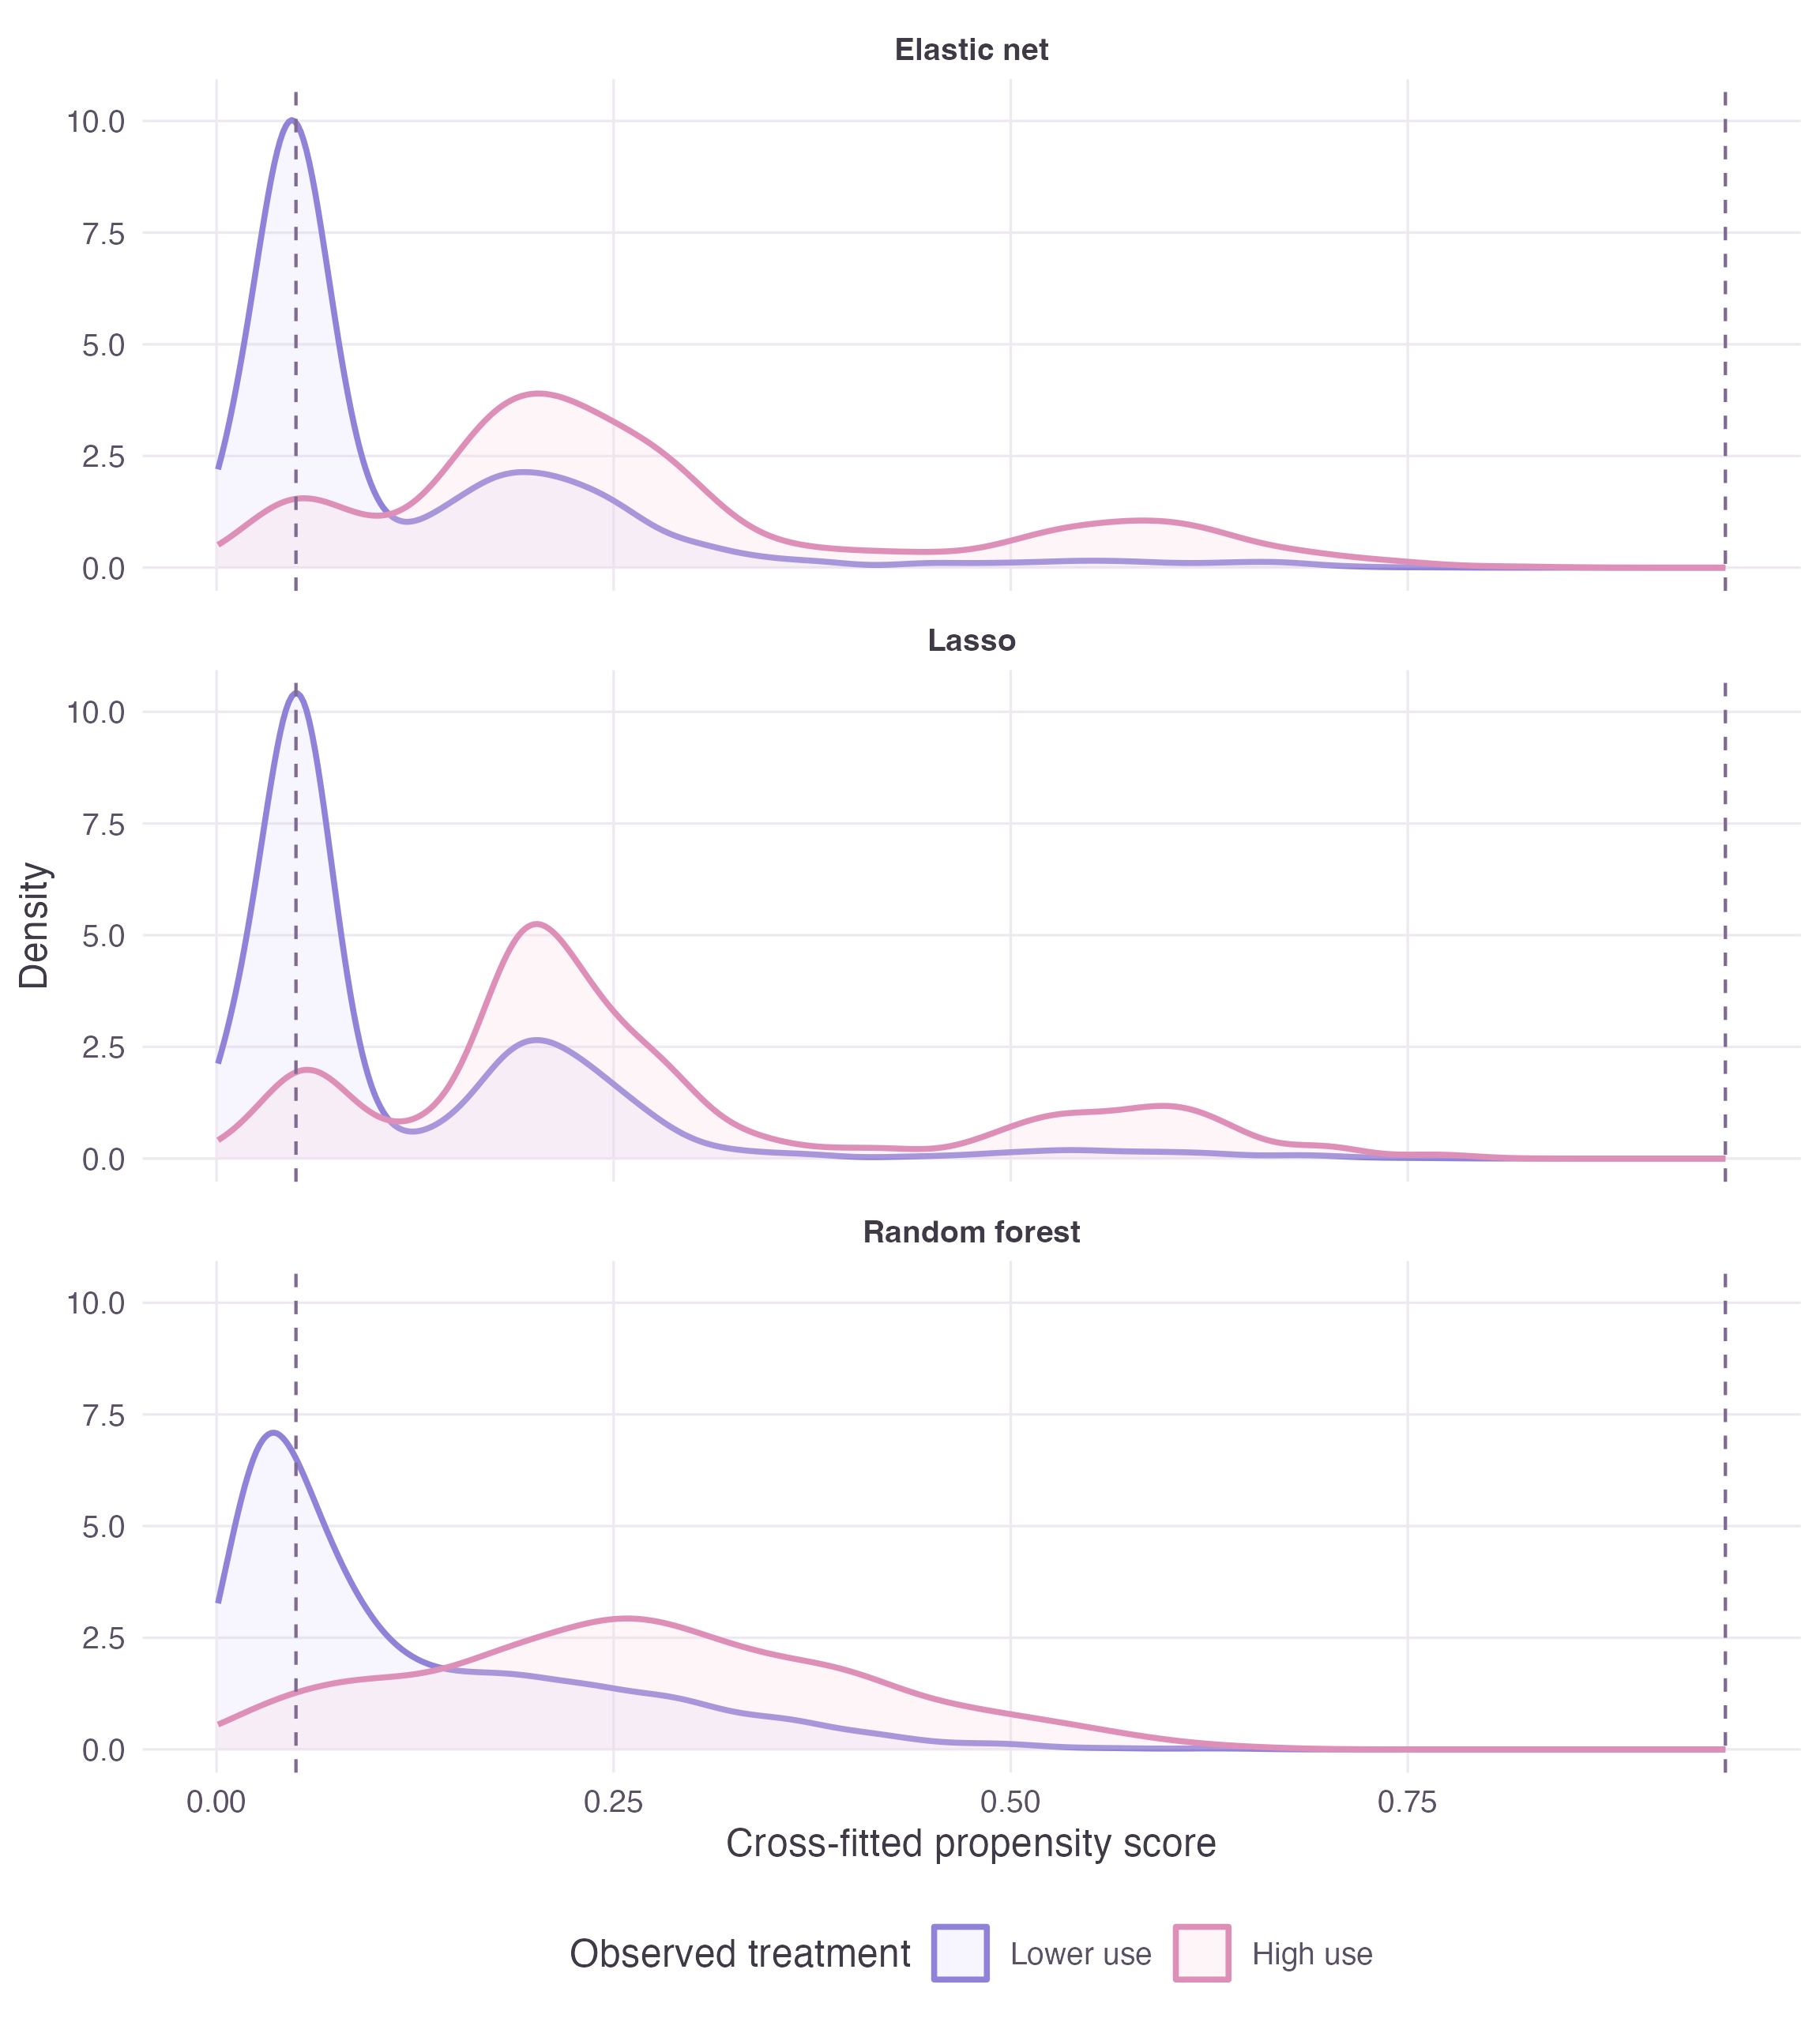
\includegraphics[width=0.80\textwidth]{figures/robustness_irm_overlap_life.png}
\caption{Cross-fitted propensity-score distributions for the binary high-use treatment}
\label{fig:robustness_irm_overlap}
\begin{minipage}{0.90\textwidth}
\footnotesize Notes: Curves show the estimated propensity-score distributions separately for adolescents observed below and above the high-use threshold. Dashed lines mark propensities of \(0.05\) and \(0.95\). The models use the rich Waves \texttt{l}--\texttt{o} controls and respondent-level five-fold cross-fitting.
\end{minipage}
\end{figure}

\begin{table}[!htbp]
\centering
\caption{IRM propensity-truncation robustness for life dissatisfaction}
\label{tab:robustness_irm_trimming}
\small
\setlength{\tabcolsep}{7pt}
\begin{tabular}{lccc}
\hline
Propensity threshold & Elastic net & Lasso & Random forest
\\
\hline
Default & 0.168 (0.121) & 0.224 (0.138) & -0.017 (0.205)
\\
1\% & 0.191* (0.111) & 0.230** (0.112) & 0.144 (0.128)
\\
2.5\% & 0.186** (0.087) & 0.224*** (0.085) & 0.196** (0.096)
\\
5\% & 0.169** (0.071) & 0.215*** (0.072) & 0.222*** (0.068)
\\
10\% & 0.159*** (0.051) & 0.203*** (0.052) & 0.242*** (0.051)
\\
\hline
\end{tabular}
\begin{minipage}{0.96\textwidth}
\footnotesize Notes: Estimated propensity scores are truncated to the interval defined by each threshold before evaluating the ATE score. The default threshold is $10^{-12}$ and reproduces the main IRM folds; all rows within a learner use the same fold partition. Cells report IRM-DML estimates with respondent-clustered standard errors in parentheses. $^{***}p<0.01$, $^{**}p<0.05$, $^{*}p<0.10$.
\end{minipage}
\end{table}


\begin{table}[!htbp]
\centering
\caption{Omitted-variable sensitivity of the PLR-DML estimates}
\label{tab:robustness_plr_sensitivity}
\small
\setlength{\tabcolsep}{7pt}
\begin{tabular}{lccc}
\hline
Learner & Estimate & Robustness value & 5\% confounding bound
\\
\hline
Elastic net & 0.060 & 3.56\% & [-0.025, 0.145]
\\
Lasso & 0.056 & 3.36\% & [-0.028, 0.141]
\\
Random forest & 0.054 & 3.27\% & [-0.029, 0.137]
\\
Neural net & 0.046 & 2.85\% & [-0.035, 0.127]
\\
\hline
\end{tabular}
\begin{minipage}{0.96\textwidth}
\footnotesize Notes: The robustness value is the common nonparametric partial $R^2$ strength with treatment and outcome required for an adversarial omitted confounder to move the point estimate to zero. The final column sets both sensitivity parameters to 5\% and uses $\rho=1$. These are point-identification bounds and do not remove the need for the unconfoundedness assumption.
\end{minipage}
\end{table}


\backmatter
\addcontentsline{toc}{chapter}{Bibliography}
\renewcommand{\baselinestretch}{1} 
\bibliographystyle{apalike}
\IfFileExists{BibTeXTemplate.bib}{\bibliography{BibTeXTemplate}}{
\chapter*{Bibliography}
Bibliographic entries will be added once the bibliography file is linked to this project.
}

\end{document}
